% Options for packages loaded elsewhere
\PassOptionsToPackage{unicode}{hyperref}
\PassOptionsToPackage{hyphens}{url}
\PassOptionsToPackage{dvipsnames,svgnames,x11names}{xcolor}
%
\documentclass[
  12pt,
]{report}

\usepackage{amsmath,amssymb}
\usepackage{iftex}
\ifPDFTeX
  \usepackage[T1]{fontenc}
  \usepackage[utf8]{inputenc}
  \usepackage{textcomp} % provide euro and other symbols
\else % if luatex or xetex
  \usepackage{unicode-math}
  \defaultfontfeatures{Scale=MatchLowercase}
  \defaultfontfeatures[\rmfamily]{Ligatures=TeX,Scale=1}
\fi
\usepackage{lmodern}
\ifPDFTeX\else  
    % xetex/luatex font selection
\fi
% Use upquote if available, for straight quotes in verbatim environments
\IfFileExists{upquote.sty}{\usepackage{upquote}}{}
\IfFileExists{microtype.sty}{% use microtype if available
  \usepackage[]{microtype}
  \UseMicrotypeSet[protrusion]{basicmath} % disable protrusion for tt fonts
}{}
\makeatletter
\@ifundefined{KOMAClassName}{% if non-KOMA class
  \IfFileExists{parskip.sty}{%
    \usepackage{parskip}
  }{% else
    \setlength{\parindent}{0pt}
    \setlength{\parskip}{6pt plus 2pt minus 1pt}}
}{% if KOMA class
  \KOMAoptions{parskip=half}}
\makeatother
\usepackage{xcolor}
\setlength{\emergencystretch}{3em} % prevent overfull lines
\setcounter{secnumdepth}{-\maxdimen} % remove section numbering
% Make \paragraph and \subparagraph free-standing
\ifx\paragraph\undefined\else
  \let\oldparagraph\paragraph
  \renewcommand{\paragraph}[1]{\oldparagraph{#1}\mbox{}}
\fi
\ifx\subparagraph\undefined\else
  \let\oldsubparagraph\subparagraph
  \renewcommand{\subparagraph}[1]{\oldsubparagraph{#1}\mbox{}}
\fi


\providecommand{\tightlist}{%
  \setlength{\itemsep}{0pt}\setlength{\parskip}{0pt}}\usepackage{longtable,booktabs,array}
\usepackage{calc} % for calculating minipage widths
% Correct order of tables after \paragraph or \subparagraph
\usepackage{etoolbox}
\makeatletter
\patchcmd\longtable{\par}{\if@noskipsec\mbox{}\fi\par}{}{}
\makeatother
% Allow footnotes in longtable head/foot
\IfFileExists{footnotehyper.sty}{\usepackage{footnotehyper}}{\usepackage{footnote}}
\makesavenoteenv{longtable}
\usepackage{graphicx}
\makeatletter
\def\maxwidth{\ifdim\Gin@nat@width>\linewidth\linewidth\else\Gin@nat@width\fi}
\def\maxheight{\ifdim\Gin@nat@height>\textheight\textheight\else\Gin@nat@height\fi}
\makeatother
% Scale images if necessary, so that they will not overflow the page
% margins by default, and it is still possible to overwrite the defaults
% using explicit options in \includegraphics[width, height, ...]{}
\setkeys{Gin}{width=\maxwidth,height=\maxheight,keepaspectratio}
% Set default figure placement to htbp
\makeatletter
\def\fps@figure{htbp}
\makeatother
% definitions for citeproc citations
\NewDocumentCommand\citeproctext{}{}
\NewDocumentCommand\citeproc{mm}{%
  \begingroup\def\citeproctext{#2}\cite{#1}\endgroup}
\makeatletter
 % allow citations to break across lines
 \let\@cite@ofmt\@firstofone
 % avoid brackets around text for \cite:
 \def\@biblabel#1{}
 \def\@cite#1#2{{#1\if@tempswa , #2\fi}}
\makeatother
\newlength{\cslhangindent}
\setlength{\cslhangindent}{1.5em}
\newlength{\csllabelwidth}
\setlength{\csllabelwidth}{3em}
\newenvironment{CSLReferences}[2] % #1 hanging-indent, #2 entry-spacing
 {\begin{list}{}{%
  \setlength{\itemindent}{0pt}
  \setlength{\leftmargin}{0pt}
  \setlength{\parsep}{0pt}
  % turn on hanging indent if param 1 is 1
  \ifodd #1
   \setlength{\leftmargin}{\cslhangindent}
   \setlength{\itemindent}{-1\cslhangindent}
  \fi
  % set entry spacing
  \setlength{\itemsep}{#2\baselineskip}}}
 {\end{list}}
\usepackage{calc}
\newcommand{\CSLBlock}[1]{\hfill\break\parbox[t]{\linewidth}{\strut\ignorespaces#1\strut}}
\newcommand{\CSLLeftMargin}[1]{\parbox[t]{\csllabelwidth}{\strut#1\strut}}
\newcommand{\CSLRightInline}[1]{\parbox[t]{\linewidth - \csllabelwidth}{\strut#1\strut}}
\newcommand{\CSLIndent}[1]{\hspace{\cslhangindent}#1}

\usepackage{kpfonts} % police kp personnalisée
\usepackage{geometry} % setup des marges du document
\usepackage{fancyhdr} % modif des headers/footers
\usepackage{titling} % setup du pre/post title
\usepackage{tikz}
\usepackage{caption} % cutomise les caption
\usepackage{xcolor}
\usepackage{fontspec} % dépendance de FontAwesome
\usepackage{fontawesome5} % icones FontAwesome

%% Définition des couleurs
\definecolor{light}{HTML}{EEEEEE}
\definecolor{highlight}{HTML}{750E21}
\definecolor{dark}{HTML}{393E46}
\definecolor{titles}{HTML}{222831}
\definecolor{StackOgray}{HTML}{e3e6e8}
\definecolor{colgraph1}{HTML}{4e6766}
\definecolor{colgraph2}{HTML}{a5c882}
\definecolor{colgraph3}{HTML}{5ab1bb}

%% Définition des marges, headers et footers
\geometry{a4paper, left=20mm, top=25mm, bottom=20mm, right=20mm}
\pagestyle{fancy}
\fancyhead{}
\renewcommand{\headrulewidth}{0pt} % retire la ligne du fancy header
\fancyfoot[R]{\includegraphics[width=30pt]{imgs/MECEN_logo.png}}
%\fancyfoot[L]{\faIcon{creative-commons-by}}

%% Page de garde
\pretitle{
    \vspace{-7.5em}
    \begin{center}
        \LARGE{\textsc{Master Économiste d'Entreprise}\\
        \vspace{2em}}
        \begin{minipage}[t]{0.6\textwidth}
            \includegraphics[width=\textwidth,height=0.25\textheight,keepaspectratio]{imgs/UT_logo.jpg}
        \end{minipage}%
        \begin{minipage}[t]{0.4\textwidth}
            \raisebox{0.15\height}{\includegraphics[width=\textwidth,height=0.11\textheight,keepaspectratio]{imgs/MECEN_logo.png}}
        \end{minipage}\\
        \vspace{7.5em}
        \Large{\textsc{Recherche, Réalisation, Restitution}}
        \vspace{5em}\\
        \rule{16cm}{2pt}\vspace{1em}
}

\posttitle{\rule{16cm}{2pt}\end{center}}


%% Améliore la commande `text`
\renewcommand{\texttt}[1]{\colorbox{light}{\color{highlight}{\ttfamily{#1}}}}

%% Améliore la commande footnote
\renewcommand*{\thefootnote}{\textcolor{highlight}{(\arabic{footnote})}}

%% Ajoute la commande pour faire ***
\newcommand{\macrostars}{
    \vspace{2em}
    \begin{center}
        \textcolor{highlight!80!black}{\Large{$\ast\ast\ast$}}
    \end{center}
}

%% Commande de divider
\newcommand{\divider}{\setlength{\parindent}{0pt}\textcolor{StackOgray!30}{\rule{\linewidth}{0.6pt}}\smallskip}


%% Caption de Figure et Table customisée
\DeclareCaptionFormat{myformat}{\textcolor{highlight}{\textbf{Figure \thefigure} $-$ }\ #3}
\captionsetup[figure]{format=myformat}

\DeclareCaptionFormat{mytableformat}{\textcolor{highlight}{\textbf{Table \thetable} $-$ }\ #3}
\captionsetup[table]{format=mytableformat}

%% Customisation du titre des chapitres
\makeatletter
\renewcommand{\chapter}{%
    \clearpage % Nouvelle page avant chaque chapitre
    \@startsection{chapter}%
    {0} % Niveau de sectionnement
    {0mm} % Indentation du titre
    {-\baselineskip} % Espace avant
    {2\baselineskip} % Espace après
    {\normalfont\Huge\bfseries | \Huge\bfseries}% Style du titre avec le symbole "|"
}
\makeatother
\usepackage{booktabs}
\usepackage{longtable}
\usepackage{array}
\usepackage{multirow}
\usepackage{wrapfig}
\usepackage{float}
\usepackage{colortbl}
\usepackage{pdflscape}
\usepackage{tabu}
\usepackage{threeparttable}
\usepackage{threeparttablex}
\usepackage[normalem]{ulem}
\usepackage{makecell}
\usepackage{xcolor}
\makeatletter
\@ifpackageloaded{tcolorbox}{}{\usepackage[skins,breakable]{tcolorbox}}
\@ifpackageloaded{fontawesome5}{}{\usepackage{fontawesome5}}
\definecolor{quarto-callout-color}{HTML}{909090}
\definecolor{quarto-callout-note-color}{HTML}{0758E5}
\definecolor{quarto-callout-important-color}{HTML}{CC1914}
\definecolor{quarto-callout-warning-color}{HTML}{EB9113}
\definecolor{quarto-callout-tip-color}{HTML}{00A047}
\definecolor{quarto-callout-caution-color}{HTML}{FC5300}
\definecolor{quarto-callout-color-frame}{HTML}{acacac}
\definecolor{quarto-callout-note-color-frame}{HTML}{4582ec}
\definecolor{quarto-callout-important-color-frame}{HTML}{d9534f}
\definecolor{quarto-callout-warning-color-frame}{HTML}{f0ad4e}
\definecolor{quarto-callout-tip-color-frame}{HTML}{02b875}
\definecolor{quarto-callout-caution-color-frame}{HTML}{fd7e14}
\makeatother
\makeatletter
\@ifpackageloaded{caption}{}{\usepackage{caption}}
\AtBeginDocument{%
\ifdefined\contentsname
  \renewcommand*\contentsname{Table des matières}
\else
  \newcommand\contentsname{Table des matières}
\fi
\ifdefined\listfigurename
  \renewcommand*\listfigurename{Liste des Figures}
\else
  \newcommand\listfigurename{Liste des Figures}
\fi
\ifdefined\listtablename
  \renewcommand*\listtablename{Liste des Tables}
\else
  \newcommand\listtablename{Liste des Tables}
\fi
\ifdefined\figurename
  \renewcommand*\figurename{Figure}
\else
  \newcommand\figurename{Figure}
\fi
\ifdefined\tablename
  \renewcommand*\tablename{Table}
\else
  \newcommand\tablename{Table}
\fi
}
\@ifpackageloaded{float}{}{\usepackage{float}}
\floatstyle{ruled}
\@ifundefined{c@chapter}{\newfloat{codelisting}{h}{lop}}{\newfloat{codelisting}{h}{lop}[chapter]}
\floatname{codelisting}{Listing}
\newcommand*\listoflistings{\listof{codelisting}{Liste des Listings}}
\makeatother
\makeatletter
\makeatother
\makeatletter
\@ifpackageloaded{caption}{}{\usepackage{caption}}
\@ifpackageloaded{subcaption}{}{\usepackage{subcaption}}
\makeatother
\ifLuaTeX
\usepackage[bidi=basic]{babel}
\else
\usepackage[bidi=default]{babel}
\fi
\babelprovide[main,import]{french}
% get rid of language-specific shorthands (see #6817):
\let\LanguageShortHands\languageshorthands
\def\languageshorthands#1{}
\ifLuaTeX
  \usepackage{selnolig}  % disable illegal ligatures
\fi
\usepackage{bookmark}

\IfFileExists{xurl.sty}{\usepackage{xurl}}{} % add URL line breaks if available
\urlstyle{same} % disable monospaced font for URLs
\hypersetup{
  pdftitle={ },
  pdfauthor={ et  },
  pdflang={fr},
  pdfkeywords={Stochastic Frontier Analysis, Hedonic Pricing, Product
Efficiency, Smartphones},
  colorlinks=true,
  linkcolor={highlight},
  filecolor={Maroon},
  citecolor={highlight},
  urlcolor={highlight},
  pdfcreator={LaTeX via pandoc}}

\title{\Huge \textbf{\textsf{Application des modèles SFA\\ à l'étude des prix}}
\vspace{5em}}
\author{\textit{Corentin DUCLOUX} et \textit{Aybuké BICAT} \vspace{2em}}
\date{29 mars 2024}

\begin{document}
\maketitle

\renewcommand*\contentsname{Table des matières}
{
\hypersetup{linkcolor=}
\setcounter{tocdepth}{2}
\tableofcontents
}
\newpage

\chapter{Remerciements}\label{remerciements}

Nous tenons à remercier chaleureusement Monsieur
\href{https://fr.linkedin.com/in/alain-bousquet-95466769}{\emph{Alain
BOUSQUET}} pour son accompagnement tout au long de ce projet
\textbf{3R}, qui a toujours été ouvert à l'exploration de nouveaux
sujets, à l'expérimentation, et nous a encouragé à creuser diverses
pistes de réflexion. Ce sujet a été et sera pour nous l'occasion de
mettre en pratique l'ensemble des connaissances acquises dans notre
cursus universitaire (microéconomie, économétrie, statistiques, analyse
de la concurrence, pricing, développement logiciel sous
\faIcon{r-project} et \texttt{python} \faIcon{python}) sur une
problématique éminemment appliquée.

\macrostars

\vspace{35em}

\emph{Note} : Ce \textbf{PDF} a été entièrement rédigé en utilisant
\texttt{Quarto}\footnote{\texttt{Quarto} : Système de publication
  technique et scientifique \emph{open-source} \(\Rightarrow\)
  \url{https://quarto.org/}.}, combinant la puissance et la versatilité
de R, Python, et \LaTeX. Une présentation interactive \texttt{reveal.js}
du sujet est aussi disponible.\footnote{Retrouvez la présentation sur
  \url{https://corentinducloux.fr/Reveal.js/slides_smartphones.html}.}

\chapter{Introduction}\label{introduction}

En tant que consommateur, nous nous retrouvons souvent face à une
question infiniment plus complexe qu'elle n'en a l'air. En des termes
simples, elle se traduit par : Pourquoi ce prix ? Pour quelle raison ce
stylo, cette nouvelle télévision, ou ce smartphone coûte tant ? Est-ce
une simple question de coût de production, de marge ? Ou bien cela
prend-il en compte d'autres éléments, tels que la valeur perçue par le
consommateur, les caractéristiques spécifiques d'un produit, ou encore
le service qu'il rend ?

Dans ce cadre, une approche essentielle dans l'analyse des prix est
celle des prix hédoniques. Celle-ci considère que le prix d'un bien ou
d'un service est influencé non seulement par ses caractéristiques, mais
aussi par la valeur subjective que les individus accordent à ces
caractéristiques. Ainsi, la méthode des prix hédoniques examine comment
des éléments spécifiques tels que la qualité ou les fonctionnalités d'un
produit impactent sa valeur perçue, reflétée dans son prix.

La compréhension des mécanismes sous-jacents à la détermination des prix
dans un marché est d'une importance cruciale tant pour les consommateurs
que pour les entreprises. Face à ces interrogations, les modèles SFA
\emph{(Stochastic Frontier Analysis)} émergent comme un outil puissant,
permettant d'évaluer et d'analyser l'efficacité des prix des produits en
allant bien au-delà d'une simple évaluation du coût de production. Ces
modèles supposent que les prix sont à l'équilibre, et prennent en compte
à la fois les valorisations du côté des consommateurs et les coûts de
production du côté des producteurs pour comprendre comment se forment
réellement les prix.

En ce sens, les modèles SFA, dans le cadre de l'étude des prix, entrent
en synergie avec l'approche hédonique en permettant une analyse
approfondie des différentes composantes qui influencent la formation des
prix.

\macrostars
\vspace{2em}

Ainsi, cette étude se déroulera en trois étapes clés : une revue de la
littérature portant sur les modèles SFA et la notion de prix hédonique.
Ensuite, nous nous concentrerons sur le processus de délimitation de
notre problématique d'étude (\emph{le marché des smartphones}). Enfin,
nous aborderons l'acquisition des données, les statistiques descriptives
et la modélisation économétrique pour comprendre plus en détail les
mécanismes de fixation des prix dans le contexte complexe et évolutif
des smartphones.

\chapter{Revue de la littérature}\label{revue-de-la-littuxe9rature}

\section{Une nouvelle approche de la théorie du
consommateur}\label{une-nouvelle-approche-de-la-thuxe9orie-du-consommateur}

En microéconomie, dans la théorie du consommateur \emph{classique}, le
choix du meilleur ensemble de consommation dépend des préférences d'un
individu. Les préférences de cet individu sont classiquement
représentées par la fonction d'utilité :

\begin{equation}\phantomsection\label{eq-umax}{
U(x) = U(x_1, x_2, \dots, x_n)
}\end{equation}

Avec \(x_1, x_2, \dots, x_n\) un vecteur de \(n\) biens.
L'équation~\ref{eq-umax} exprime donc la relation entre la quantité de
biens consommés et le niveau d'utilité que ces biens procurent à un
agent. Dès lors, dans ce cadre, la consommation de biens procure
\textbf{directement} de l'utilité à l'agent. En pratique pourtant, il
est difficile de concevoir comment l'achat d'un bien comme une lampe ou
un stylo peut nous apporter de l'utilité en tant que consommateur.

Pour répondre à cette difficulté, Lancaster
(\citeproc{ref-lancaster1966}{1966}) propose un nouveau cadre conceptuel
théorique décrit par les hypothèses suivantes.

\begin{tcolorbox}[enhanced jigsaw, colframe=quarto-callout-tip-color-frame, colbacktitle=quarto-callout-tip-color!10!white, left=2mm, rightrule=.15mm, toprule=.15mm, bottomtitle=1mm, breakable, colback=white, titlerule=0mm, coltitle=black, arc=.35mm, opacitybacktitle=0.6, opacityback=0, bottomrule=.15mm, leftrule=.75mm, toptitle=1mm, title=\textcolor{quarto-callout-tip-color}{\faLightbulb}\hspace{0.5em}{Hypothèses}]

\begin{enumerate}
\def\labelenumi{\arabic{enumi}.}
\tightlist
\item
  Le bien en lui-même ne procure pas d'utilité au consommateur
  \(\Rightarrow\) il possède des \textbf{caractéristiques} qui procurent
  de l'utilité.
\item
  Un bien est un ensemble (\emph{bundle}) de caractéristiques \(-\) il
  possède le plus souvent de nombreuses caractéristiques.
\item
  Une combinaison de biens peut procurer une utilité qui n'est pas la
  simple somme des utilités procurées par les biens séparément.
\end{enumerate}

\end{tcolorbox}

\emph{Illustrons ces points avec quelques exemples} :

\begin{itemize}
\item
  Un ordinateur n'est pas acheté pour le simple plaisir de posséder un
  ordinateur. Il est acheté car il permet de naviguer sur Internet,
  écrire des cours, programmer, regarder une série, etc. C'est donc pour
  les \textbf{services qu'il nous rend}, ce qui est modélisé ici par les
  caractéristiques possédées du bien.
\item
  Les biens possèdent généralement un grand nombre de caractéristiques.
  Prenons l'exemple d'une gourde : la couleur, la forme, les dimensions
  et la capacité isothermique sont autant de caractéristiques qui
  peuvent influer sur la décision d'achat et la disposition à payer.
\item
  En consommant du lait et du café séparément, les caractéristiques
  retirées du lait sont de la vitamine D et du calcium, tandis que pour
  le café les caractéristiques retirées sont de la caféine, une boisson
  chaude, un \emph{``boost''} le matin. En revanche, consommer un café
  latte permettra d'obtenir une boisson plus douce, moins caféiné, un
  goût différent. En bref, les caractéristiques retirées du mélange sont
  différentes.
\end{itemize}

Dans le modèle de Lancaster, on pose une relation \textbf{linéaire}
entre les prix des biens et leurs caractéristiques. Le prix total \(p\)
d'un bien peut donc être considéré comme la somme des prix individuels
associé à chaque caractéristique. Cela découle du fait que les attributs
des biens étudiés peuvent être considérés comme des composantes
distinctes et séparables.

\section{Pricing Hédonique}\label{pricing-huxe9donique}

\subsection{Aspects théoriques}\label{aspects-thuxe9oriques}

Rosen (\citeproc{ref-rosen1974}{1974}) étend ce qui a été apporté par le
cadre théorique de Lancaster (\citeproc{ref-lancaster1966}{1966}). La
principale différence est qu'il s'intéresse à \textbf{l'équilibre de
marché de biens différenciés} (là où Lancaster s'intéresse uniquement à
la demande) avec :

\begin{itemize}
\item
  un continuum de biens du côté de l'offre.
\item
  un continuum de consommateurs hétérogènes du côté de la demande.
\end{itemize}

Dans ce modèle, la relation entre les prix des biens et leurs attributs
peut-être \textbf{non-linéaire} et permet aussi de capter des effets
d'interaction entre plusieurs variables. Au coût d'une modélisation plus
complexe que dans le modèle de Lancaster
(\citeproc{ref-lancaster1966}{1966}), les résultats gagnent en
robustesse.

L'objet de la contribution de Rosen est d'étudier un bien différencié
\(z\) décrit par le vecteur de ses \(n\) caractéristiques mesurables tel
que :

\begin{equation}\phantomsection\label{eq-hedonic}{
z = (z_1, z_2, \dots, z_n)
}\end{equation}

Afin de comprendre pourquoi il est important d'étudier des biens
différenciés dans ce cadre, regardons en détail le graphique suivant.

\begin{figure}

\centering{

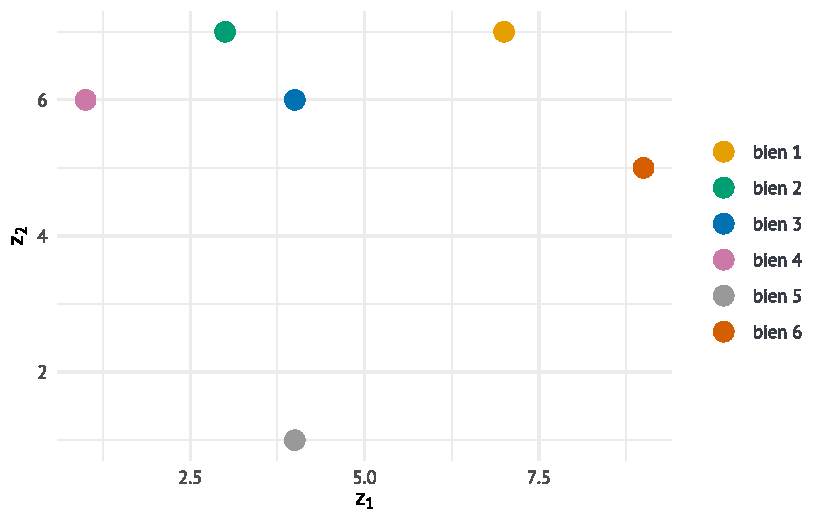
\includegraphics{report_files/figure-pdf/fig-hedonic-1.pdf}

}

\caption{\label{fig-hedonic}Plan \((z_1, z_2)\) de différents biens avec
2 caractéristiques.}

\end{figure}%

En général, nous sommes habitués à représenter les préférences des
consommateurs en termes de quantités de biens \(x_1, x_2\). Ici, on
assiste à un changement de paradigme : on va représenter les préférences
des consommateurs en termes de caractéristiques de biens, c'est-à-dire
dans l'espace \(z_1, z_2\) (on choisit de prendre seulement 2
caractéristiques et 6 biens pour simplifier).

On peut en déduire que les consommateurs achetant le \emph{bien 5}
valorisent plus les caractéristiques \(z_1\) que \(z_2\), et inversement
pour le \emph{bien 4}.

\emph{En fait, la différenciation horizontale et verticale des produits
implique qu'une vaste gamme de paniers est disponible dans cet espace de
consommation !}

\begin{itemize}
\item
  \textbf{Différenciation Horizontale} \(\Rightarrow\) A prix donné, il
  n'y a pas unanimité dans le choix des consommateurs entre 2 biens
  (jaune et rouge) : ce sont des différences de goûts.
\item
  \textbf{Différenciation Verticale} \(\Rightarrow\) A prix donné, il y
  a unanimité dans le choix des consommateurs entre 2 voitures biens :
  l'un est meilleur que l'autre.
\end{itemize}

Il faut aussi noter que dans le modèle de Rosen, le consommateur
n'achète qu'\textbf{une seule} unité de bien qui est une combinaison
d'attributs \(z_1, z_2, \dots, z_n\). Historiquement, cela s'explique
car Rosen s'intéresse principalement aux biens durables (logements,
voitures, smartphones\ldots). Il est en effet beaucoup plus simple
d'obtenir des caractéristiques observables sur ces biens durables : que
ce soit le nombre de pièces pour un logement, la superficie, ou bien la
puissance et la longueur d'une voiture.

De toutes ces informations, on peut formuler 2 questions.

\begin{itemize}
\tightlist
\item
  Pour le \textbf{producteur}, quelle combinaison de caractéristiques
  lui permet de maximiser son profit ?
\item
  Pour le \textbf{consommateur}, quelle combinaison de caractéristiques
  lui rapporte le plus d'utilité sous contrainte budgétaire ?
\end{itemize}

On aboutit à une relation fonctionnelle entre les caractéristiques des
biens et leur prix, appelée fonction de prix hédonique \(p(z)\).

\begin{equation}\phantomsection\label{eq-price}{
\boxed{p(z) = p(z_1, z_2, \dots, z_n)}
}\end{equation}

Un produit est donc défini en chaque point du plan et guide les choix de
localisation des consommateurs et des producteurs concernant les
ensembles de caractéristiques.

\begin{tcolorbox}[enhanced jigsaw, colframe=quarto-callout-warning-color-frame, colbacktitle=quarto-callout-warning-color!10!white, left=2mm, rightrule=.15mm, toprule=.15mm, bottomtitle=1mm, breakable, colback=white, titlerule=0mm, coltitle=black, arc=.35mm, opacitybacktitle=0.6, opacityback=0, bottomrule=.15mm, leftrule=.75mm, toptitle=1mm, title=\textcolor{quarto-callout-warning-color}{\faExclamationTriangle}\hspace{0.5em}{Limites}]

Il n'en reste pas moins qu'il subsiste un problème indéniable : ce qu'on
aimerait réellement mesurer c'est le \textbf{service rendu par un
produit} \emph{(pour lequel le lien précis entre ses fonctionnalités et
les services rendus reste inconnu)} et non pas les caractéristiques de
ce produit. Mais ce premier est complètement inobservable. Un défi sera
donc d'interpréter correctement les résultats des régressions.

\end{tcolorbox}

\subsection{Application}\label{application}

Harrison Jr et Rubinfeld (\citeproc{ref-harrison1978}{1978}) :

\textbf{Objectif} : Examiner comment les données du marché immobilier
peuvent être utilisées pour évaluer la \emph{Willingness To Pay} des
consommateurs pour une meilleure qualité de l'air.

\begin{itemize}
\tightlist
\item
  Le modèle suppose que les ménages prennent en compte le niveau de
  pollution de l'air, la quantité et la qualité du logement et d'autres
  caractéristiques de quartier pour faire leur choix.
\end{itemize}

\newpage

\begin{itemize}
\tightlist
\item
  La fonction de la valeur hédonique du logement traduit les attributs
  du logement en prix, et suppose que les consommateurs perçoivent avec
  précision ces attributs et que le marché est en équilibre à court
  terme.
\end{itemize}

\emph{Définition des variables}

\begin{itemize}
\tightlist
\item
  \(W\) = WTP \emph{marginale} pour une meilleure qualité de l'air
\item
  \(NOX\) = Concentration des oxydes d'azote\footnote{Variable de
    pollution, \(NOX\) est un \emph{proxy} pour la qualité de l'air.}
\item
  \(INC\) = Revenu du ménage en centaine de dollars
\end{itemize}

Trois niveaux de revenu par an découpés en variable catégorielles :

\begin{itemize}
\tightlist
\item
  \textbf{LOW} si \(INC\) \(\leq \$\) 8500 \(\Rightarrow Y_0\)
  (Catégorie de référence)
\item
  \textbf{MEDIUM} si \(INC\) \(\leq \$\) 11500 \(\Rightarrow Y_1\)
\item
  \textbf{HIGH} si \(INC\) \(\leq \$\) 15000 \(\Rightarrow Y_2\)
\end{itemize}

\begin{equation}\phantomsection\label{eq-WTP1}{
\log(W) = \beta_0 + \beta_1 \log(NOX) + \beta_2 \log(INC) + \beta_3[Y_1 \cdot \log(NOX)] + \beta_4[Y_2 \cdot \log(NOX)]
}\end{equation}

Coefficients estimés pour la régression \(\log-\log\) (significatifs au
seuil \(p<0.01\)) :

\[
\log(W) = \underbrace{2.2}_{\beta_0} + \underbrace{0.97}_{\beta_1} \log(NOX) + \underbrace{0.8}_{\beta_2} \log(INC) - \underbrace{0.03}_{\beta_3}[Y_1 \cdot \log(NOX)] - \underbrace{0.07}_{\beta_4}[Y_2 \cdot \log(NOX)]
\]

\textbf{Résultats} : La WTP marginale pour une meilleure qualité de
l'air augmente avec le niveau de pollution de l'air et avec le niveau de
revenu des ménages. Plus précisément, malgré la présence d'effets
d'interaction significatifs mais faibles, il est observé que toutes
choses égales par ailleurs, lorsque le niveau de \(NOX\) et le revenu du
ménage augmentent, le prix a tendance à augmenter également.

\begin{center}\rule{0.5\linewidth}{0.5pt}\end{center}

Pour finir, l'approche hédonique a été utilisée empiriquement dans de
très nombreux domaines comme par exemple :

Berndt et Rappaport (\citeproc{ref-berndt2001}{2001}) \(\Rightarrow\)
Secteur informatique.

\begin{itemize}
\tightlist
\item
  L'objectif de cet article est d'examiner l'évolution des prix ajustés
  en qualité des ordinateurs personnels de bureau et mobiles entre 1976
  et 1999.
\end{itemize}

Chen et Rothschild (\citeproc{ref-chen2010}{2010}) \(\Rightarrow\)
Secteur de l'hôtellerie.

\begin{itemize}
\tightlist
\item
  Analyse l'impact des caractéristiques des hôtels de Taipei sur leurs
  tarifs en utilisant les données de 73 hôtels collectées auprès d'un
  agent de voyage en ligne.
\end{itemize}

Yim, Lee, et Kim (\citeproc{ref-yim2014}{2014}) \(\Rightarrow\) Secteur
de la restauration.

\begin{itemize}
\tightlist
\item
  Explore l'impact des attributs des restaurants à Séoul sur leurs prix
  moyens de repas en examinant les données de 185 établissements
  recueillies via diverses sources.
\end{itemize}

Dans la littérature, une spécification \emph{semi-log} est généralement
préférée en raison de sa capacité à mieux modéliser les relations non
linéaires entre les variables. De plus, cette forme permet d'améliorer
l'ajustement du modèle aux données observées, et offre un \(R^2\)
supérieur à celui obtenu avec d'autres spécifications \(-\) voir Bello
et Moruf (\citeproc{ref-bello2010}{2010}).

\newpage

\section{Fonction de production}\label{fonction-de-production}

Avant de passer à l'explication de la seconde partie théorique,
c'est-à-dire les modèles SFA, attardons-nous sur la définition d'une
fonction de production, fondement important de la SFA.

\begin{tcolorbox}[enhanced jigsaw, colframe=quarto-callout-tip-color-frame, colbacktitle=quarto-callout-tip-color!10!white, left=2mm, rightrule=.15mm, toprule=.15mm, bottomtitle=1mm, breakable, colback=white, titlerule=0mm, coltitle=black, arc=.35mm, opacitybacktitle=0.6, opacityback=0, bottomrule=.15mm, leftrule=.75mm, toptitle=1mm, title=\textcolor{quarto-callout-tip-color}{\faLightbulb}\hspace{0.5em}{Rappel}]

\begin{itemize}
\item
  Un processus de production représente la transformation d'inputs en
  outputs.
\item
  Dès lors, une fonction de production \(f(.)\) donne la quantité
  maximum d'output \(y\) pouvant être produite à partir de combinaison
  d'inputs.
\end{itemize}

\end{tcolorbox}

\begin{equation}\phantomsection\label{eq-prod}{
y_i = f(x_i; \beta)
}\end{equation}

Avec \(x_i\) le vecteur d'inputs et \(\beta\) le vecteur de paramètres
inconnus à estimer.

\(f(x_i; \beta)\) est en fait la frontière de production. Pour l'instant
cette frontière ne prend pas en compte l'efficacité technique \(TE_i\)
et elle n'est pas \emph{stochastique} car elle n'inclut pas de terme
aléatoire.

\macrostars
\vspace{2em}

Farrell (\citeproc{ref-farrell1957}{1957}) est le premier auteur à
définir cette \emph{Frontière de Production}.

\begin{quote}
\emph{``When one talks about the efficiency of a firm one usually means
its success in producing as large as possible an output from a given set
of inputs.''}
\end{quote}

Cette définition permet donc d'aboutir à la formulation évoquée à
l'équation~\ref{eq-prod}.

\section{Le modèle SFA}\label{le-moduxe8le-sfa}

\subsection{Aspects théoriques}\label{aspects-thuxe9oriques-1}

Aigner, Lovell, et Schmidt (\citeproc{ref-aigner1977}{1977}) :

\textbf{Objectif} : Formulation et estimation de fonctions de frontière
de production stochastique.

Avant les travaux de Aigner, Lovell, et Schmidt
(\citeproc{ref-aigner1977}{1977}), les économètres utilisaient
principalement dans la littérature des fonctions de production pour
étudier le lien entre le niveau de production et la quantité d'inputs
utilisés. Cela signifie que la formulation théorique énoncée par Farrell
(\citeproc{ref-farrell1957}{1957}) différait de l'utilisation empirique.
En effet, Farrell (\citeproc{ref-farrell1957}{1957}) a lui introduit la
notion d'efficacité au sens du \textbf{niveau maximum de production}
atteignable étant donné une combinaison spécifique d'inputs.

\begin{itemize}
\tightlist
\item
  On repart de la fonction de production (équation~\ref{eq-prod}), mais
  en lui ajoutant un terme multiplicatif \(TE_i\).
\end{itemize}

\[{\displaystyle y_{i}=f(x_{i};\beta )\cdot TE_{i}}\]

\(TE_i\) représente l'efficacité technique, définie comme le ratio
d'output observé sur l'output maximum réalisable, soit
\(TE_i = \dfrac{y_i}{y_i^*}\).

\begin{itemize}
\tightlist
\item
  Si \(TE_i = 1\) alors la firme \(i\) produit l'output maximum
  réalisable, alors que si \(TE_i < 1\), il existe un écart entre
  l'output maximum et l'output effectivement observé.
\end{itemize}

Un composant \textbf{stochastique} \({\exp \left\{{v_{i}}\right\}}\) est
en outre ajouté pour représenter les chocs aléatoires affectant la
production. La fonction de production devient alors :

\[{\displaystyle y_{i}=f(x_{i};\beta )\cdot TE_{i}\cdot \exp \left\{{v_{i}}\right\}}\]

On peut ré-écrire l'efficacité technique sous la forme
\({\displaystyle TE_{i}=\exp \left\{{-u_{i}}\right\}}\). Dès lors :

\begin{equation}\phantomsection\label{eq-sfa}{
\boxed{{\displaystyle y_{i}=f(x_{i};\beta )\cdot \exp \left\{{-u_{i}}\right\}\cdot \exp \left\{{v_{i}}\right\}}}
}\end{equation}

\emph{Note} : En réarrangeant l'équation~\ref{eq-sfa} avec le logarithme
népérien, on obtient :

\(\Leftrightarrow \ln(y_i) = \ln(f(x_i;\beta)) + \underbrace{v_i -u_i}_{\epsilon_i}\)

Le modèle peut alors s'écrire sous la forme suivante :
\begin{equation}\phantomsection\label{eq-log-sfa}{
\boxed{\ln(y_i) = \ln(f(x_i;\beta)) + \epsilon_i}
}\end{equation}

L'avantage de cette écriture est qu'elle facilite la manipulation des
termes d'erreur, et il est très simple de retrouver le logarithme de
l'output maximum. En effet :

\(\Leftrightarrow \ln(y_i) = \underbrace{\ln(f(x_i;\beta)) + v_i}_{\ln(y_i^*)} -u_i\)

Et donc le logarithme de l'output observé est simplement
\(\ln(y_i) = \ln(y_i^*) -u_i\).

Les termes d'erreur \(\epsilon_i\) ont ainsi une distribution
particulière composée :

\begin{itemize}
\item
  \(v_i\) est une \textbf{erreur aléatoire} \(\Rightarrow\) variation
  inexpliquée par les variables indépendantes du modèle, avec
  \(v_i \sim \mathcal{N}(0, \sigma^2_v)\).
\item
  \(u_i\) est un \textbf{composant unilatéral} qui peut être choisi
  parmi plusieurs distributions\footnote{Dans la littérature, deux
    distributions sont couramment utilisées : la distribution
    \textbf{semi-normale} et \textbf{normale tronquée}.} et
  \(u_i \geq 0\), puisqu'il est nécessaire d'avoir \(TE_i ≤ 1\).
\end{itemize}

\begin{tcolorbox}[enhanced jigsaw, colframe=quarto-callout-tip-color-frame, colbacktitle=quarto-callout-tip-color!10!white, left=2mm, rightrule=.15mm, toprule=.15mm, bottomtitle=1mm, breakable, colback=white, titlerule=0mm, coltitle=black, arc=.35mm, opacitybacktitle=0.6, opacityback=0, bottomrule=.15mm, leftrule=.75mm, toptitle=1mm, title=\textcolor{quarto-callout-tip-color}{\faLightbulb}\hspace{0.5em}{Conclusion}]

Pour chaque observation dans ce modèle, on récupère \(\epsilon_i\), qui
représente un écart à la frontière. La spécification de cette méthode
permet donc d'estimer, à travers l'espérance conditionnelle de \(u_i\)
sachant \(\epsilon_i\), les scores de l'\textbf{efficacité technique} de
chaque firme.

\end{tcolorbox}

Enfin, Kumbhakar, Horncastle, et al.
(\citeproc{ref-kumbhakar2015}{2015}) discutent aussi dans la section
\textbf{3.3} de leur livre des approches dites \emph{distribution-free}
sur \(u_i\) dans lesquelles aucune hypothèse ne sont faites sur la
distribution que suit les \(u_i\). Nous ne nous intéresserons pas à ces
méthodes puisqu'elles ont le défaut de ne pas pouvoir correctement
distinguer les \(v_i\) des \(u_i\), et donc ne sont pas en mesure
d'estimer les scores d'efficacité technique.

\newpage

On l'a vu ci-dessus, la SFA est une méthode \textbf{paramétrique} qui
requiert une forme fonctionnelle précise. La SFA n'a cependant pas le
monopole dans le domaine de l'estimation des frontières de production.

Un autre modèle (non-paramétrique) a aussi été développé : la Data
Envelopment Analysis (DEA). Celui-ci a l'avantage de ne pas exiger
d'hypothèse particulière sur des termes d'erreur. La structure du modèle
n'est pas spécifiée à priori mais est uniquement déterminée à partir des
données.

\macrostars
\vspace{2em}

\begin{figure}[htbp]
    \centering
    \includegraphics[width=0.8\textwidth]{imgs/stochastic_image.jpeg}
    \caption{Représentation graphique d'une SFA.}
    \label{fig:example}
\end{figure}

\(*\) Droits d'auteur :
\href{https://www.researchgate.net/profile/Lutz-Bornmann}{Lutz Bornmann}

À partir de cette représentation, on peut clairement distinguer les
effets de \(v_i\) (\texttt{noise}) et ceux de \(u_i\)
(\texttt{inefficiency}) dans un espace à deux dimensions avec \(X\) la
quantité d'inputs et \(Y\) la quantité d'outputs. La frontière optimale
de production est ici représentée en noir par
\(y = \beta_0 + \beta_1x\).

\begin{itemize}
\item
  2 entreprises utilisant la même quantité d'inputs (\(X=3\)) sont mises
  en évidence dans le graph. La première se situe en dessous de la
  frontière de production avec \(Y \simeq 2\) et la seconde est
  au-dessus de celle-ci avec \(Y>6\).
\item
  Les 2 firmes utilisent donc la même quantité d'inputs pour une
  quantité d'output différente, à savoir : la première firme est moins
  efficace dans l'utilisation optimale de ses inputs, donc son
  efficacité technique est inférieure à la seconde.
\end{itemize}

\newpage

\subsection{Utilisation empirique}\label{utilisation-empirique}

\textbf{Quelques exemples d'application de la SFA dans le cadre de la
mesure d'efficacité} :

Reinhard, Lovell, et Thijssen (\citeproc{ref-reinhard2000}{2000})
\(\Rightarrow\) Secteur Environnemental.

\begin{itemize}
\tightlist
\item
  L'objectif de cet article est d'estimer l'efficacité environnementale
  pour les fermes laitières aux Pays-Bas.
\end{itemize}

Rosko et Mutter (\citeproc{ref-rosko2008}{2008}) \(\Rightarrow\) Secteur
Hospitalier.

\begin{itemize}
\tightlist
\item
  Cet article est quant à lui une méta-analyse de l'ensemble des
  articles de SFA et de DEA existants sur l'efficacité hospitalière aux
  Etats-Unis.
\end{itemize}

Mohamad, Hassan, et Bader (\citeproc{ref-mohamad2008}{2008})
\(\Rightarrow\) Secteur Bancaire.

\begin{itemize}
\tightlist
\item
  Compare l'efficacité des coûts et des profits de 80 banques dans 21
  pays comprenant 37 banques conventionnelles et 43 banques islamiques.
\end{itemize}

\begin{center}\rule{0.5\linewidth}{0.5pt}\end{center}

\textbf{En bref, il existe de nombreux domaines d'application} !

Un domaine en particulier n'a pourtant pas été évoqué jusqu'ici :
pourquoi ne pas utiliser la SFA pour mesurer l'\emph{efficacité} d'un
prix \textbf{(best-buy frontier)} ?

C'est précisément le cadre du prochain article de notre revue de la
littérature.

\section{SFA \& Pricing Hédonique}\label{sfa-pricing-huxe9donique}

Arrondo, Garcia, et Gonzalez (\citeproc{ref-arrondo2018}{2018}) :

\textbf{Objectif} : déterminer les attributs principaux des prix des
sneakers en Espagne et leur efficacité.

Six caractéristiques\footnote{Variables quantitatives discrètes
  \(\in [1,10[\).} sont étudiées sur \(n=171\) sneakers.

\begin{itemize}
\item
  \textbf{Lightweight} : poids des sneakers.
\item
  \textbf{Cushioning} : capacité de la chaussure à absorber les chocs au
  cours d'une course et tout au long du cycle de vie du produit.
\item
  \textbf{Flexibility} : les baskets flexibles s'adaptent mieux à la
  forme naturelle du pied.
\item
  \textbf{Response} : capacité du matériau à retrouver sa forme après
  les déformations provoquées par l'impact sur le sol.
\item
  \textbf{Grip} : l'adhérence donne aux coureurs une certaine assise sur
  le sol.
\item
  \textbf{Stability} : mesure la stabilité du pied à l'intérieur de la
  chaussure.
\end{itemize}

En plus de ces 6 caractéristiques techniques, la marque est ajoutée en
tant que variable qualitative pour mesurer la \emph{Brand Equity} (la
valeur d'une marque pour le consommateur).

\newpage

Le modèle pour la marque \(k\) s'écrit alors :

\begin{equation}\phantomsection\label{eq-arrondo}{
\ln(p_{ik}) = \alpha_k + \beta X_{ik} + v_{ik} + u_{ik}
}\end{equation}

\begin{itemize}
\tightlist
\item
  \(p_{ik}\) est le prix du \(i\)-ème modèle de marque \(k\).
\item
  \(α_k\) est l'effet marque sur le prix de la marque \(k\).
\item
  \(X_{ik}\) est le vecteur des attributs mesurables du \(i\)-ème modèle
  de marque \(k\).
\item
  \(β\) est un vecteur de coefficients pour ces attributs.
\item
  \(v_{ik}\) est une erreur aléatoire.
\item
  \(u_{ik}\) représente l'inefficacité.
\end{itemize}

\emph{Note} : On retrouve bien la forme spécifique d'une SFA,
caractérisée par la présence des termes \(v_{ik}\) et \(u_{ik}\). La
seule différence est que le terme d'erreur composée est
\(\epsilon_{ik} = v_{ik} + u_{ik}\) car nous sommes dans le cadre d'une
\textbf{frontière de coût} et non de production.

\begin{center}\rule{0.5\linewidth}{0.5pt}\end{center}

\textbf{Résultats} :

\begin{longtable}[]{@{}lll@{}}
\caption{Résultats de la régression
hédonique}\label{tbl-arrondo-hedonic}\tabularnewline
\toprule\noalign{}
\textbf{Variables} & Coefficient & \(SE\) \\
\midrule\noalign{}
\endfirsthead
\toprule\noalign{}
\textbf{Variables} & Coefficient & \(SE\) \\
\midrule\noalign{}
\endhead
\bottomrule\noalign{}
\endlastfoot
\emph{Lightness} & 0.007 & 0.028 \\
\emph{Cushioning} & 0.064 ** & 0.025 \\
\emph{Flexibility} & 0.058 ** & 0.026 \\
\emph{Response} & 0.050 * & 0.30 \\
\emph{Stability} & 0.070 *** & 0.025 \\
\emph{Grip} & -0.045 & 0.028 \\
\texttt{Adidas} & 2.697 *** & 0.401 \\
\texttt{Asics} & 2.679 *** & 0.389 \\
\texttt{Saucony} & 2.779 *** & 0.403 \\
\texttt{Nike} & 2.714 *** & 0.422 \\
\texttt{Brooks} & 2.834 *** & 0.404 \\
\texttt{Mizuno} & 2.524 *** & 0.397 \\
\texttt{New\ Balance} & 2.544 *** & 0.410 \\
\texttt{Reebok} & 2.522 *** & 0.403 \\
\end{longtable}

Les variables \emph{Cushioning}, \emph{Flexibility} et \emph{Stability}
sont statistiquement significatives à \(p<0.05\).

De plus, nous sommes ici dans le cadre d'une régression
\(\log\)-linéaire donc les coefficients peuvent être interpretés comme
des \textbf{semi-élasticités}, c'est à dire :

\(\Rightarrow\) Pour une augmentation d'une unité de \emph{Stability},
\(p_{ik}\) va augmenter de 7\%, \emph{cet. par.}\footnote{\emph{Toutes
  choses égales par ailleurs}.}

\(\Rightarrow\) Pour une augmentation d'une unité de \emph{Cushioning},
\(p_{ik}\) va augmenter de 6.4\%, \emph{cet. par.}

\(\Rightarrow\) Pour une augmentation d'une unité de \emph{Flexibility},
\(p_{ik}\) va augmenter de 5.8\%, \emph{cet. par.}

Par conséquent, la caractéristique \emph{Stability} va avoir le plus
grand impact sur le prix d'une sneakers, suivi de \emph{Cushioning} et
\emph{Flexibility}.

\begin{longtable}[]{@{}ll@{}}
\caption{Indice d'efficacité moyen par
marque}\label{tbl-arrondo-brand}\tabularnewline
\toprule\noalign{}
\textbf{Marque} & \(\hat{\theta_k}\) \\
\midrule\noalign{}
\endfirsthead
\toprule\noalign{}
\textbf{Marque} & \(\hat{\theta_k}\) \\
\midrule\noalign{}
\endhead
\bottomrule\noalign{}
\endlastfoot
\texttt{Adidas} (\(n=\) 28) & 0.832 \\
\texttt{Asics} (\(n=\) 35) & 0.864 \\
\texttt{Saucony} (\(n=\) 15) & 0.875 \\
\texttt{Nike} (\(n=\) 25) & 0.824 \\
\texttt{Brooks} (\(n=\) 16) & 0.860 \\
\texttt{Mizuno} (\(n=\) 29) & 0.858 \\
\texttt{New\ Balance} (\(n=\) 18) & 0.848 \\
\texttt{Reebok} (\(n=\) 5) & 0.859 \\
\end{longtable}

\(\hat{\theta_k}\) représente l'indice d'efficacité moyen estimé par
marque, compris entre 0 et 1.

On remarque tout d'abord que cet indice est compris entre 0.8 et 0.9
pour l'ensemble des marques, c'est à dire qu'il n'y a pas de marque
globalement \textbf{très inefficiente} (si une marque l'était, elle
n'arriverait probablement pas à vendre et serait évincée par ses
concurrents).

\begin{itemize}
\tightlist
\item
  \texttt{Nike} est la marque qui possède la pire relation
  prix\textasciitilde attributs de la sélection.
\item
  \texttt{Saucony} est la marque qui possède la meilleure relation
  prix\textasciitilde attributs de la sélection.
\end{itemize}

\textbf{Résultats}

\begin{itemize}
\item
  En estimant l'efficacité des produits, l'article permet de déterminer
  le montant des réductions à accorder aux sneakers \textbf{overprice}
  afin de les rendre compétitives.
\item
  Il existe une relation inverse entre l'efficacité du produit et la
  réduction de prix : la réduction de prix est d'autant plus grande que
  la sneakers est \textbf{overprice}.
\end{itemize}

\chapter{Choix et cadrage de la
problématique}\label{choix-et-cadrage-de-la-probluxe9matique}

L'objectif fixé par notre sujet est de combiner les modèles SFA à une
problématique d'étude des prix hédoniques, de manière similaire à ce qui
a été entrepris par Arrondo, Garcia, et Gonzalez
(\citeproc{ref-arrondo2018}{2018}).

L'ensemble des articles de la littérature exposés ci-dessus ont permis
d'affiner notre compréhension théorique des modèles et nous ont aidés à
déterminer un marché à étudier. Pour des raisons de disponibilité des
caractéristiques et parce que peu d'articles dans la littérature se sont
intéressés au pricing hédonique des smartphones, nous avons fait le
choix d'analyser le marché de la téléphonie mobile.

Notre problématique est donc la suivante :

\textbf{Combinaison d'un modèle SFA et d'une régression hédonique pour
évaluer l'écart entre les prix de smartphones et leur valeur
(intrinsèque).}

\section{Le marché de la téléphonie mobile, en constante
évolution}\label{le-marchuxe9-de-la-tuxe9luxe9phonie-mobile-en-constante-uxe9volution}

Depuis l'apparition des téléphones mobiles au début des années 1990, de
nombreuses innovations technologiques ont ajouté des caractéristiques
rendant ces téléphones de plus en plus polyvalents. Cette chronologie
présente en \(X\) les années et les rectangles des différentes
catégories correspondent à des \textbf{débuts} et des \textbf{fins de
commercialisation}. L'axe \(Y\) permet quant à lui d'améliorer la
lisibilité.

\begin{figure}[htbp]
    \centering
    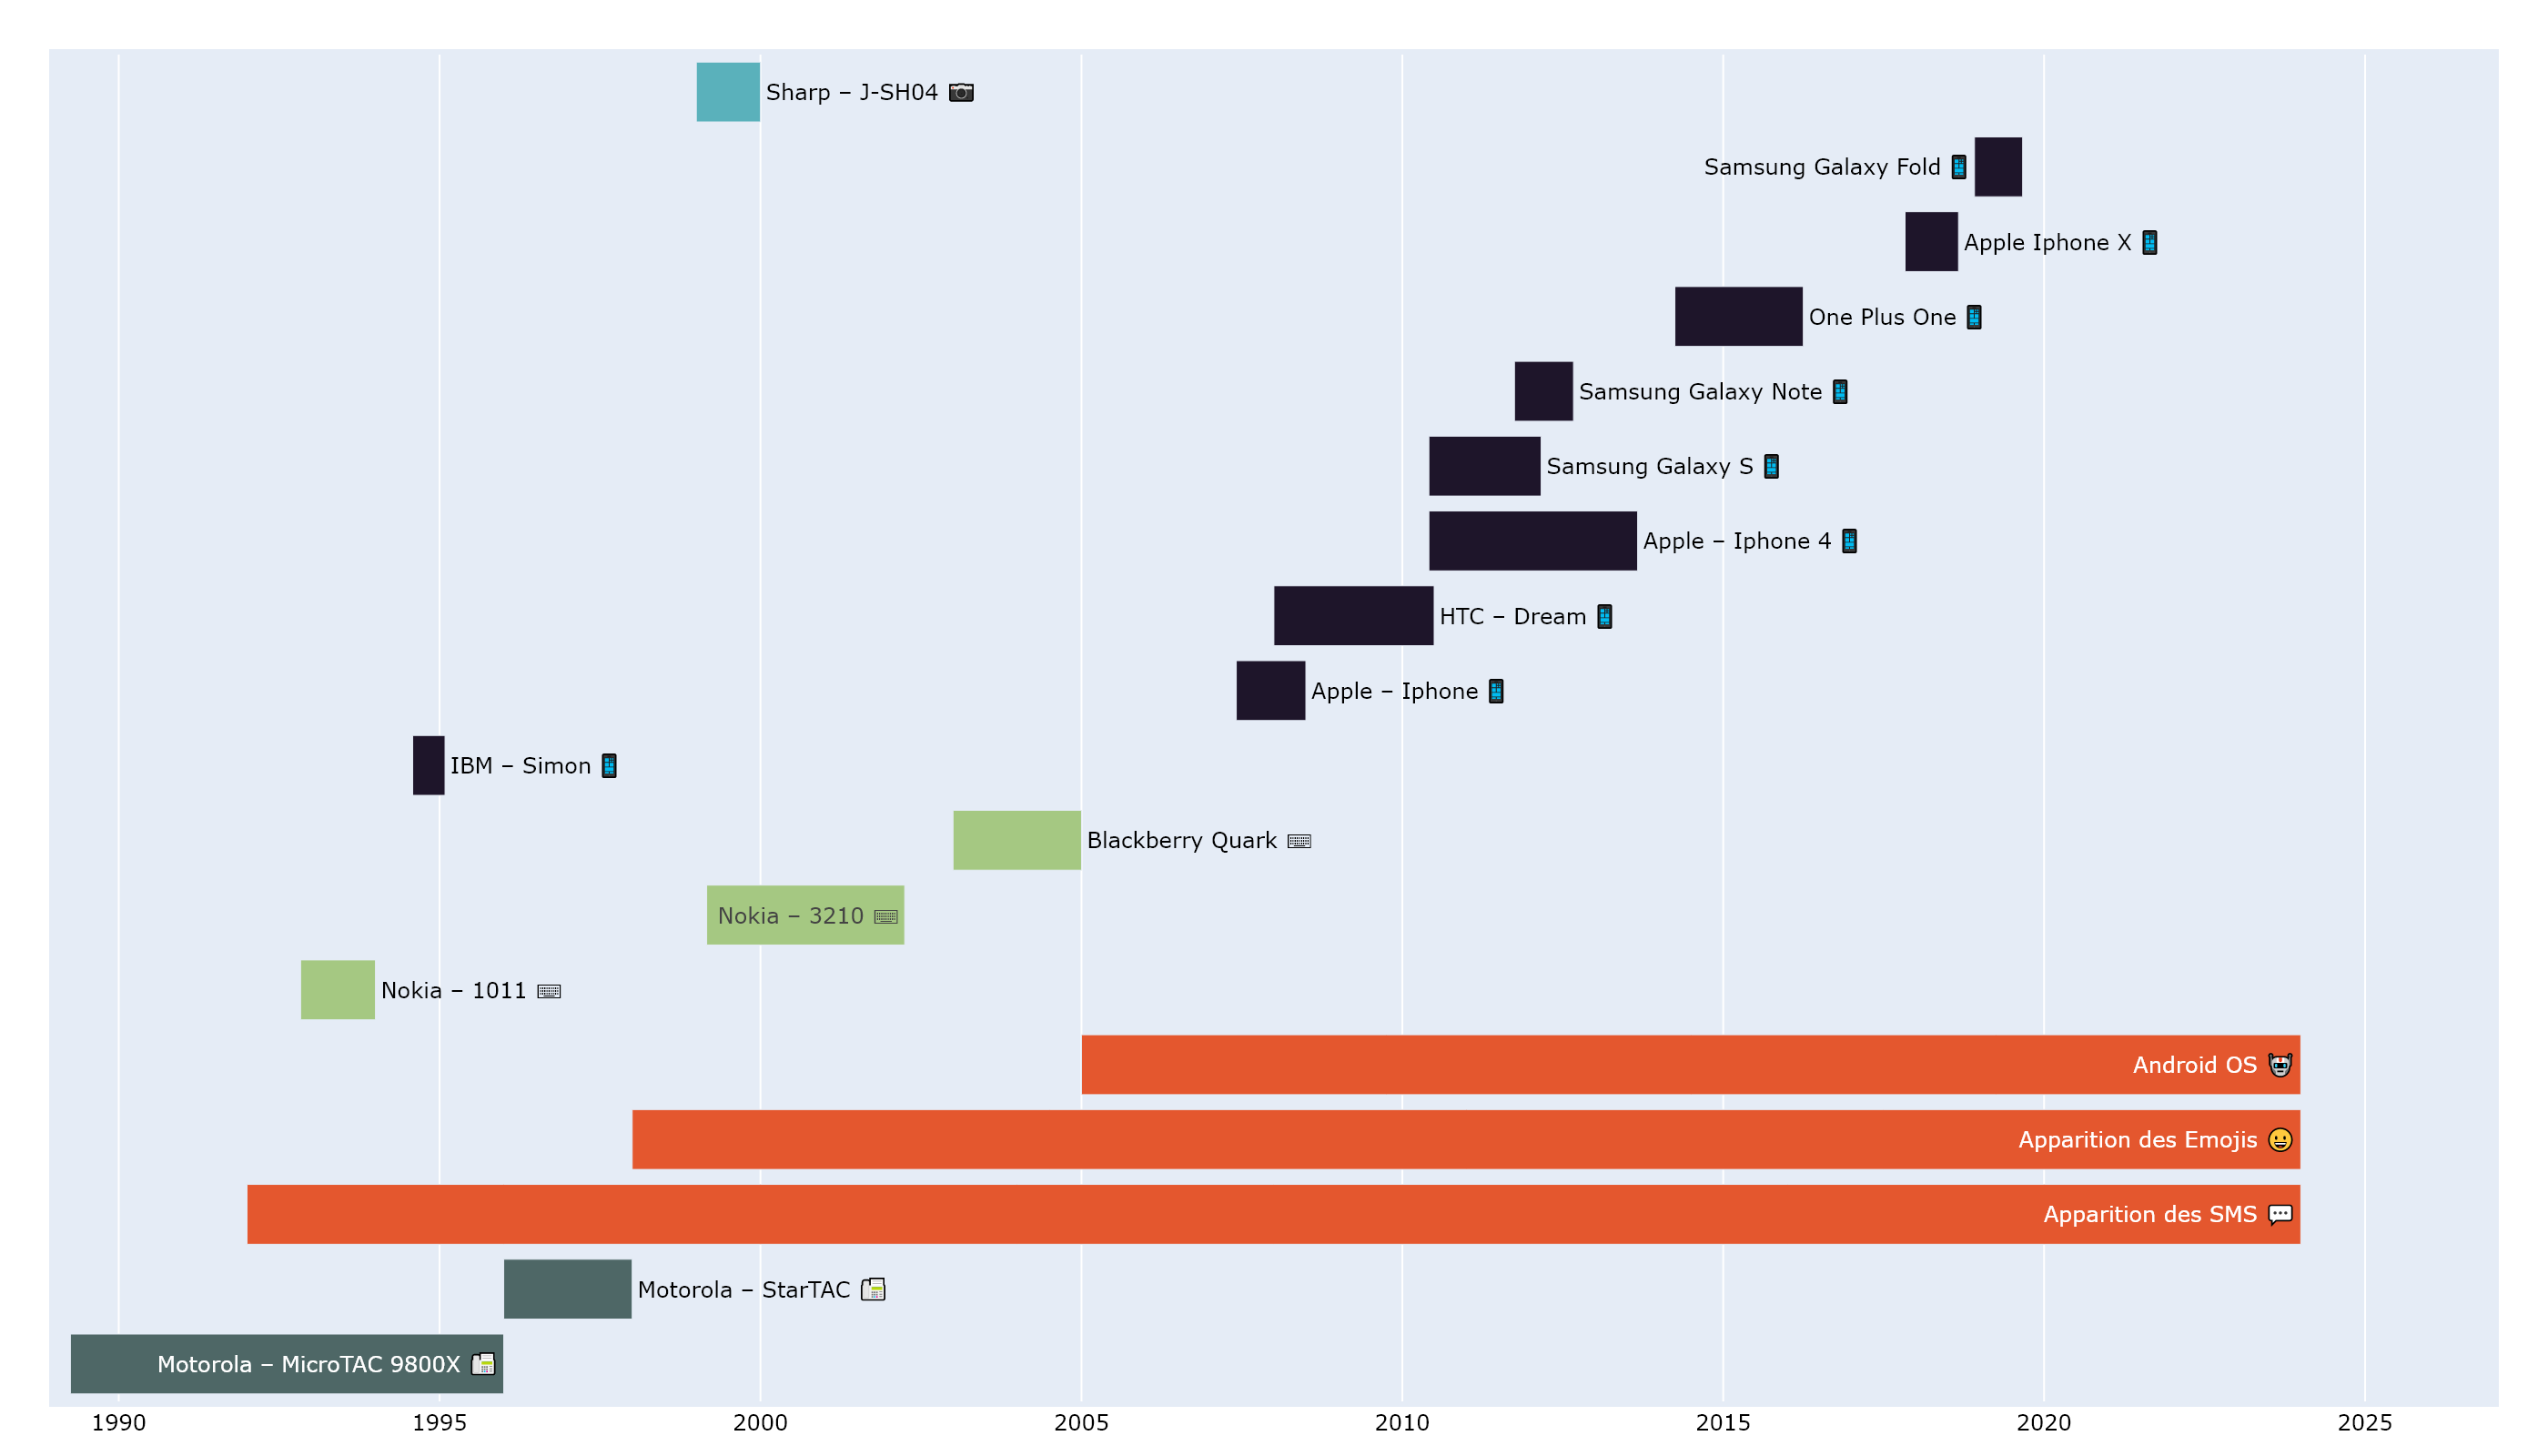
\includegraphics[width=0.99\textwidth]{imgs/smartphones_timeline.png}
    \caption{Smartphone Timeline.}
    \label{fig:smartphones}
\end{figure}

\textcolor{colgraph1}{$\blacksquare$} Téléphone à clapet
\textcolor{colgraph2}{$\blacksquare$} Téléphone à clavier
\textcolor{colgraph3}{$\blacksquare$} Téléphone à appareil photo
\(\blacksquare\) Smartphone

Examinons quelques modèles de téléphone pour mieux saisir l'impact des
innovations majeures sur le marché.

\begin{itemize}
\item
  \emph{Nokia 1011} : Premier écran LCD.
\item
  \emph{IBM Simon} : Premier véritable smartphone avec stylet,
  commercialisé pendant seulement 6 mois à cause d'un prix élevé de
  \$899.
\item
  \emph{Nokia 3210} : Premier téléphone à intégrer les SMS et plusieurs
  jeux. C'est encore aujourd'hui un des téléphones les plus vendus au
  monde.
\item
  \emph{Sharp J-SH04} : Premier téléphone équipé d'un appareil photo
  intégré.
\item
  \emph{Blackberry Quark} : Les téléphones \faIcon{blackberry}
  BlackBerry sont les premiers à disposer d'un clavier complet, ce qui,
  à cette époque, est un avantage majeur. A tel point qu'au début des
  années 2000 et jusqu'en 2010, Blackberry devient et reste leader sur
  le marché de la téléphonie mobile avec 20\% de parts de marché à son
  apogée.
\item
  \emph{Apple Iphone} : En 2007, \faIcon{apple} Apple annonce l'iPhone.
  Ce téléphone, qui intègre un écran tactile multitouch, va bouleverser
  le marché des téléphones mobiles. La vraie révolution, plus que le
  téléphone en lui-même, est l'\emph{App Store}, qui va permettre
  d'accélérer le développement de nombreuses applications mobiles.
\item
  \emph{HTC Dream} : Un an après la sortie de l'iPhone, les
  constructeurs bataillent pour tenter de le concurrencer. HTC est dans
  ce cadre le premier à intégrer Android OS. Il reste néanmoins un
  entre-deux (il possède un clavier et un écran tactile).
\item
  \emph{Samsung Galaxy S} : Avec le Galaxy S, Samsung concurrence
  directement l'Apple iPhone 4 et sort un téléphone meilleur en tout
  point sur le plan des caractéristiques techniques. L'écran est plus
  grand, il existe une possibilité d'augmenter le stockage, il possède
  un meilleur cpu et une meilleure autonomie, tout en étant moins cher.
\end{itemize}

\begin{tcolorbox}[enhanced jigsaw, colframe=quarto-callout-tip-color-frame, colbacktitle=quarto-callout-tip-color!10!white, left=2mm, rightrule=.15mm, toprule=.15mm, bottomtitle=1mm, breakable, colback=white, titlerule=0mm, coltitle=black, arc=.35mm, opacitybacktitle=0.6, opacityback=0, bottomrule=.15mm, leftrule=.75mm, toptitle=1mm, title=\textcolor{quarto-callout-tip-color}{\faLightbulb}\hspace{0.5em}{Conclusion}]

Toutes ces innovations vont avoir un impact dans les caractéristiques
les plus valorisées par les consommateurs. Par exemple, il est difficile
d'imaginer qu'un consommateur valorisera aujourd'hui un téléphone sans
capteur de caméra frontale et arrière ou qui serait incapable d'envoyer
des SMS.

\end{tcolorbox}

\vspace{2em}

Cela permet d'ailleurs d'évoquer une des limites majeures des modèles de
pricing hédonique. Comment va-t-on pouvoir modéliser l'arrivée d'une
nouvelle caractéristique ? On ne peut pas trouver dans le passé quelle
sera la valorisation de cette nouvelle caractéristique.

\emph{Illustrons cette remarque avec l'iPhone}. Un modèle de régression
des prix hédoniques réalisé juste avant la sortie de l'iPhone aurait
probablement trouvé (sans surprise) que BlackBerry était la marque la
plus valorisée par les consommateurs et qu'il faut augmenter la taille
du téléphone pour lui permettre d'avoir un plus grand clavier. Il va
sans dire que deux mois plus tard, ces résultats sont inutilisables à
cause d'une innovation technologique.

Enfin, il existe relativement peu d'articles sur les prix hédoniques des
smartphones, ou alors ils sont assez anciens (2004-2005), et on l'a vu,
étant donné la vitesse à laquelle évolue le marché, avoir des données
récentes est primordial pour estimer correctement les caractéristiques
valorisées par les consommateurs à un instant \(T\).

\newpage

\section{Smartphones et Pricing
Hédonique}\label{smartphones-et-pricing-huxe9donique}

Il existe néanmoins quelques articles récents traitant du sujet, dont
celui de Ahmad, Ahmed, et Ahmad (\citeproc{ref-ahmad2019}{2019}) :

\textbf{Objectif} : Pricing des attributs des smartphones au Pakistan

Les données des attributs ont été collectées sur des sites webs et les
prix pratiqués relevés dans les magasins de 2 villes du Pakistan
(\(n=348\) smartphones).

Le prix moyen d'un smartphone dans leur étude est de \$136,35. En outre,
l'\textbf{écart-type} du prix des smartphones est elevé (181), c'est à
dire que la dispersion en prix est assez importante, ce qui confirme
l'hypothèse que les smartphones sont des biens différenciés.

\emph{Ils proposent alors l'estimation du modèle suivant avec les
caractéristiques découpées en variables catégorielles.}

\[
\begin{split}
\ln(PRICE_i) = \beta_0 + \beta_{1i}BRAND_i + \beta_{2i}WEIGHT_i + \beta_{3i}BATTERY_i \\
+ \beta_{4i}OS_i + \beta_{5i}RAM_i + \beta_{6i}MEMORY_i + \beta_{7i}DISPLAY_i \\
+ \beta_{8i}NETWORK_i + \beta_{9i}BCAM_i + \beta_{10i}FCAM_i + \epsilon_i
\end{split}
\]

\textbf{Résultats} :

\begin{itemize}
\tightlist
\item
  La marque, la batterie, le poids, l'OS, la RAM, la mémoire et la
  taille de l'écran ont un effet positif statistiquement significatif
  sur les prix des smartphones.
\end{itemize}

Plus précisément, les résultats indiquent que les fabricants doivent se
concentrer sur un téléphone :

\begin{itemize}
\tightlist
\item
  avec une RAM de plus d'1 Go.
\item
  avec une mémoire de plus de 8 Go.
\item
  avec un écran de plus de 5 pouces.
\item
  compatible avec la 4G.
\item
  avec une caméra arrière de plus de 15 mégapixels.
\end{itemize}

\begin{center}\rule{0.5\linewidth}{0.5pt}\end{center}

Le Pakistan étant un pays en voie de développement, et l'étude datant de
2019, on peut s'attendre à trouver des résultats différents dans nos
données.

De plus, sur les 348 smartphones, 127, sont de la marque
\textbf{QMOBILE}, une société pakistanaise qui vend des smartphones à
bas prix, ce qui peut aussi expliquer le prix moyen assez bas.

\section{Effet de réputation}\label{effet-de-ruxe9putation}

Dans la section précédente, les résultats de l'étude de Ahmad, Ahmed, et
Ahmad (\citeproc{ref-ahmad2019}{2019}) ont permis de discerner que la
marque a un effet statistiquement significatif sur le prix des
smartphones, c'est pourquoi nous voulions explorer rapidement des
questions d'analyse de la concurrence que l'on peut relier à notre
sujet.

Boistel (\citeproc{ref-boistel2008}{2008}) parle spécifiquement de cet
effet de réputation.

\textbf{Objectif :} Analyser l'impact de la réputation sur les fonctions
clés de l'entreprise et son intégration dans le management stratégique
actuel.

\textbf{Réputation et marketing}

\begin{itemize}
\item
  \textbf{Considéré comme une priorité majeure} : la réputation est une
  ressource essentielle, reconnue comme une priorité de recherche par le
  \emph{Marketing Science Institute}.
\item
  \textbf{Influence le comportement des consommateurs}: la réputation
  impacte l'intention d'achat, la confiance envers les nouveaux produits
  et est liée à la satisfaction client. Elle agit comme une
  \emph{``garantie''}.
\item
  \textbf{Avantage compétitif} : une solide réputation permet de gagner
  un avantage compétitif sur le marché, voire un avantage concurrentiel,
  en attirant les clients et en se différenciant des concurrents.
\item
  \textbf{Limitation de la concurrence} : les produits ou services d'une
  entreprise réputée sont moins facilement remplaçables ou imitables en
  raison de la perception limitée des consommateurs. Au lieu d'examiner
  les caractéristiques en détail, ils vont se fier à la marque et à la
  réputation.
\item
  \textbf{Corrélation positive avec le prix} : une meilleure réputation
  va permettre de fixer des prix plus élevés et d'obtenir un avantage
  sur les ventes par rapport à la concurrence. \emph{Exemple} :
  \emph{Toyota} et \emph{General Motors} forment la joint-venture
  \emph{New United Motor Manufacturing Inc.} La société a produit 2
  voitures identiques :

  \begin{itemize}
  \tightlist
  \item
    la Toyota Corrola.
  \item
    la GM's Geo Prizm.
  \end{itemize}
\end{itemize}

\(\Rightarrow\) La meilleure réputation de Toyota lui a permis de vendre
200000 voitures à 11100 dollars, contre seulement 80000 véhicules à
10700 dollars vendus pour General Motors.

\begin{center}\rule{0.5\linewidth}{0.5pt}\end{center}

\chapter{Acquisition des données}\label{acquisition-des-donnuxe9es}

\section{Scraping}\label{scraping}

Il n'existe \textbf{évidemment} pas de données directement disponibles
regroupant le prix et l'ensemble des caractéristiques des smartphones.
Ce qui pourrait le plus s'en rapprocher sont les fiches techniques de
téléphones disponibles sur \url{https://www.01net.com/}. Scraper ce site
pourrait être une idée intéressante, mais \emph{01net} n'est pas un
revendeur de smartphones.

L'idée est donc de récupérer ces données sur le site d'un revendeur
(\emph{Fnac}, \emph{Darty}, \emph{Boulanger}). En effet, l'avantage de
la récupération des données sur un site de revente direct est que nous
avons une \emph{``photographie''} du marché au moment où le
\emph{crawler} récupère et alimente notre base de données. A ce titre,
nous avons choisi de récupérer des données sur
\href{https://www.boulanger.com/}{Boulanger}.

\begin{tcolorbox}[enhanced jigsaw, colframe=quarto-callout-warning-color-frame, colbacktitle=quarto-callout-warning-color!10!white, left=2mm, rightrule=.15mm, toprule=.15mm, bottomtitle=1mm, breakable, colback=white, titlerule=0mm, coltitle=black, arc=.35mm, opacitybacktitle=0.6, opacityback=0, bottomrule=.15mm, leftrule=.75mm, toptitle=1mm, title=\textcolor{quarto-callout-warning-color}{\faExclamationTriangle}\hspace{0.5em}{Encadrement du web scraping}]

Le web scraping est encadré en droit français par l'article \textbf{L.
342-3}\footnotemark{} du Code de la propriété intellectuelle, qui
autorise la pratique suivante :

\vspace{1em}

\begin{itemize}
\tightlist
\item
  L'extraction et la réutilisation d'une partie substantielle, appréciée
  de façon qualitative ou quantitative, à des fins exclusives
  d'illustration dans le cadre de l'enseignement et de la recherche et
  pour un public composé d'élèves, d'étudiants, d'enseignants ou de
  chercheurs directement concernés. Ainsi, \textbf{ce cas de figure
  étant limité à des fins pédagogiques, il est totalement exclu de faire
  usage des données extraites à titre commercial}.
\end{itemize}

\end{tcolorbox}

\footnotetext{\href{https://www.legifrance.gouv.fr/codes/article_lc/LEGIARTI000044365654}{Plus
de détail sur \texttt{legifrance.gouv.fr}}}

\vspace{1em}

\textbf{Nous précisons donc que nous ne ferons en aucun usage de ces
données dans un cadre commercial.}

\newpage

\section{Méthodologie}\label{muxe9thodologie}

L'objectif final est de disposer d'une application permettant aux
consommateurs ou aux producteurs de comparer l'efficacité des
smartphones en fonction de leurs caractéristiques et de leur indiquer
quel est le meilleur choix.

\textbf{Workflow} :

\begin{itemize}
\tightlist
\item
  \emph{Scraping} \(\Rightarrow\) \texttt{Python}
\item
  \emph{Nettoyage des données} \(\Rightarrow\) \texttt{Python}
\item
  \emph{Modélisation} \(\Rightarrow\) \texttt{R}
\item
  \emph{Application} \(\Rightarrow\) \texttt{Python}
\end{itemize}

\vspace{2em}

\begin{figure}[htbp]
    \centering
    \includegraphics[width=0.7\textwidth]{imgs/mermaid_graph.png}
    \caption{Diagramme fonctionnel.}
    \label{fig:method}
\end{figure}

Le diagramme fonctionnel permet de comprendre comment interagissent les
différents composants logiciels avant leur utilisation dans
l'application.

\chapter{Statistiques descriptives}\label{statistiques-descriptives}

Il y a 487 smartphones valides disponibles dans nos données scrapées sur
Boulanger avec 35 variables.

\begin{itemize}
\item
  Variables liées à l'écran : \emph{screen\_type}, \emph{screen\_size},
  \emph{screen\_tech}, \emph{diagonal\_pixels}, \emph{ppi},
  \emph{resolution\_1}, \emph{resolution\_2}.
\item
  Variables liées à la caméra : \emph{mpx\_backward\_cam},
  \emph{cam\_1}, \emph{cam\_2}, \emph{cam\_3}, \emph{sensor}.
\item
  Variables liées aux caractéristiques physiques du téléphone :
  \emph{color}, \emph{thickness}, \emph{width}, \emph{height},
  \emph{net\_weight}.
\item
  Variables liées aux performances : \emph{network}, \emph{cpu},
  \emph{ram}, \emph{storage}, \emph{upgrade\_storage}.
\item
  Variables liées à la batterie : \emph{battery}, \emph{fast\_charging},
  \emph{induction}, \emph{usb\_type\_c}.
\item
  Variables liées au DAS : \emph{das\_limbs}, \emph{das\_chest},
  \emph{das\_head}.
\item
  Autres variables : \emph{repairability\_index}, \emph{model},
  \emph{brand}, \emph{made\_in}, \emph{stars}, \emph{reviews}.
\end{itemize}

Et enfin notre variable à expliquer : \textbf{price}.

\section{Analyse des prix}\label{analyse-des-prix}

\subsection{Mesures de tendance
centrale}\label{mesures-de-tendance-centrale}

Le prix moyen d'un smartphone de la sélection est de 711.11 €, soit
\(\simeq\) 5 fois plus élevé que dans l'article de Ahmad, Ahmed, et
Ahmad (\citeproc{ref-ahmad2019}{2019}). Cela peut s'expliquer notamment
par la différence considérable de \textbf{PIB} par habitant.\footnote{Données
  issues de la
  \href{https://donnees.banquemondiale.org/indicator/NY.GDP.PCAP.CD?most_recent_year_desc=true}{\emph{Banque
  Mondiale}} (PIB par habitant en US dollars courants)}

\begin{itemize}
\tightlist
\item
  En 2022 au Pakistan : \(\$\) 1596.7
\item
  En 2022 en France : \(\$\) 40963.8
\end{itemize}

La médiane est quant à elle de 597.64 €.

\begin{figure}[H]

{\centering 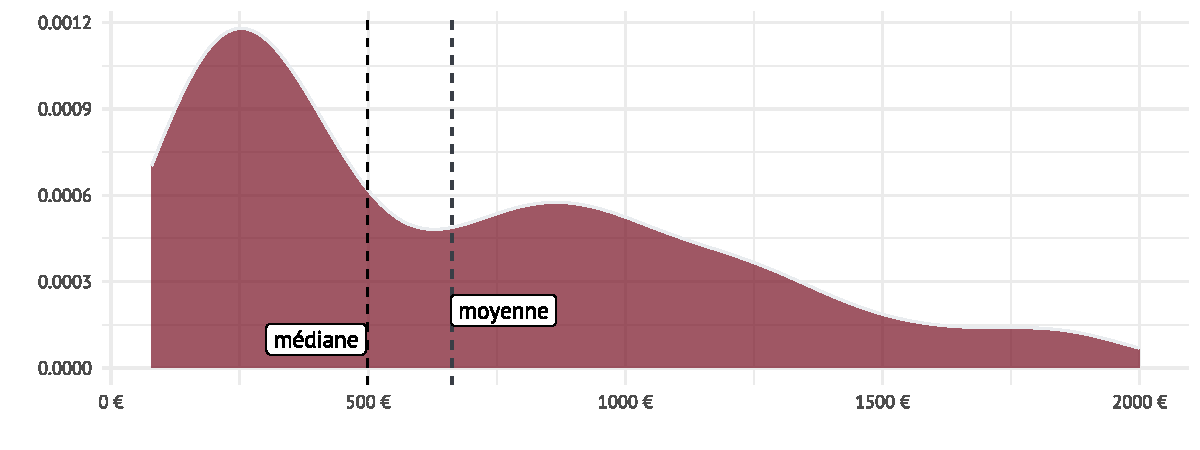
\includegraphics{report_files/figure-pdf/density_phones-1.pdf}

}

\caption{Distribution des prix des smartphones.}

\end{figure}%

On peut aussi tester l'asymétrie de la distribution avec le coefficient
de \emph{Skewness} de \emph{Pearson} :

\[SK = \dfrac{3(\bar{x} - \tilde{x})}{\sigma} \simeq 0.67\]

Ce résultat indique que l'asymétrie de la distribution est positive. Il
y a beaucoup plus de valeurs concentrées à gauche de la distribution
qu'à droite. Si le coefficient était proche de 0, cela signifierait que
la distribution est proche d'une loi normale \(\mathcal{N}\), ce qui
n'est pas le cas.

\subsection{Mesures de dispersion}\label{mesures-de-dispersion}

Le prix minimal d'un smartphone dans notre sélection est de 91.4 € pour
le modèle \textbf{Xiaomi Redmi A1} et le prix maximal est de 2279 € pour
le modèle \textbf{Samsung Galaxy Z Fold 5}.

Il existe donc une grande étendue de prix, c'est à dire : 2187.6 €. De
plus, l'écart-type du prix est très important \emph{(506.36)}.

\textbf{Toutes ces mesures nous confirment que la dispersion en prix est
très elevée.}

\subsection{Prix moyen en fonction d'autres
variables}\label{prix-moyen-en-fonction-dautres-variables}

On peut s'intéresser au prix moyen par marque pour regarder s'il existe
des différences de prix significatives entre certaines marques pour
illustrer l'article de Boistel (\citeproc{ref-boistel2008}{2008}) cité
précédemment.

\begin{figure}[H]

{\centering 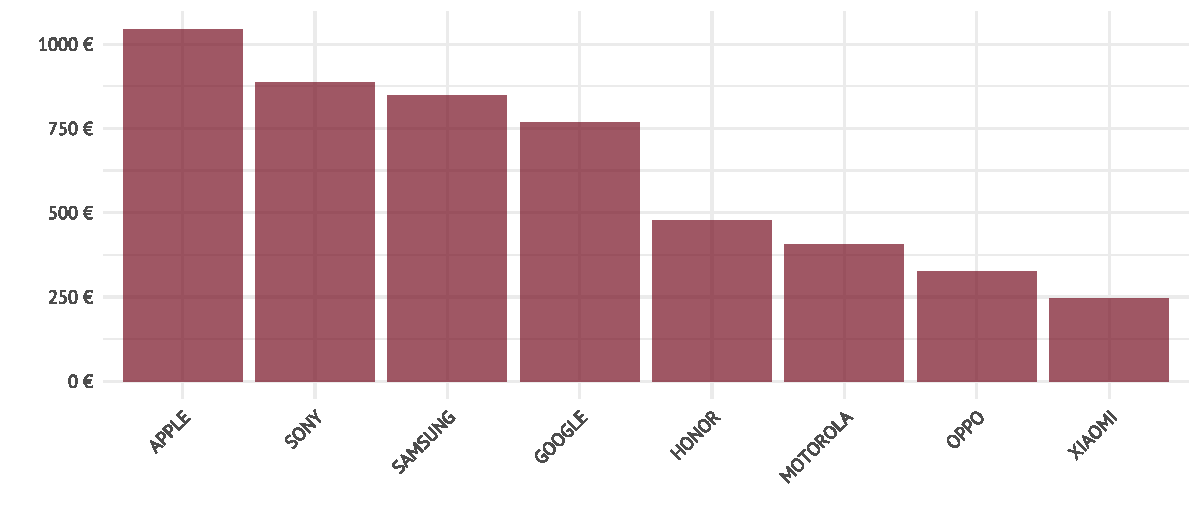
\includegraphics{report_files/figure-pdf/fig_mean_price-1.pdf}

}

\caption{Prix moyen par marque.}

\end{figure}%

\begin{itemize}
\item
  \emph{Apple} possède en moyenne les téléphones les plus chers dans
  l'échantillon (1177.75 €).
\item
  Le prix moyen des smartphones commercialisés par \emph{Samsung} est de
  848.98 €. C'est certes moins qu'\emph{Apple}, mais cela peut
  s'expliquer car \emph{Samsung} commercialise à la fois des téléphones
  très haut de gamme et des téléphones bas de gamme aux prix beaucoup
  plus attractifs.
\item
  En dernière position, on retrouve \emph{Xiaomi} avec des téléphones à
  un prix moyen aux alentours de 260 €.
\end{itemize}

\newpage

\begin{table}[!h]
\centering
\caption{\label{tab:kable_1}Prix moyen en fonction de la RAM.}
\centering
\begin{tabular}[t]{lrl}
\toprule
\textbf{ram} & \textbf{$n$} & \textbf{prix moyen $\bar p$}\\
\midrule
\cellcolor{gray!10}{2 Go} & \cellcolor{gray!10}{21} & \cellcolor{gray!10}{110.11 €}\\
3 Go & 16 & 165.35 €\\
\cellcolor{gray!10}{4 Go} & \cellcolor{gray!10}{118} & \cellcolor{gray!10}{413.4 €}\\
6 Go & 87 & 722.22 €\\
\cellcolor{gray!10}{8 Go} & \cellcolor{gray!10}{163} & \cellcolor{gray!10}{835.55 €}\\
\addlinespace
12 Go & 75 & 1144.02 €\\
\cellcolor{gray!10}{16 Go} & \cellcolor{gray!10}{7} & \cellcolor{gray!10}{1106.14 €}\\
\bottomrule
\end{tabular}
\end{table}

\begin{table}[!h]
\centering
\caption{\label{tab:kable_2}Prix moyen en fonction du stockage.}
\centering
\begin{tabular}[t]{lrl}
\toprule
\textbf{stockage} & \textbf{$n$} & \textbf{prix moyen $\bar p$}\\
\midrule
\cellcolor{gray!10}{32 Go} & \cellcolor{gray!10}{27} & \cellcolor{gray!10}{116.65 €}\\
64 Go & 55 & 214.76 €\\
\cellcolor{gray!10}{128 Go} & \cellcolor{gray!10}{207} & \cellcolor{gray!10}{537.44 €}\\
256 Go & 127 & 930.65 €\\
\cellcolor{gray!10}{512 Go} & \cellcolor{gray!10}{55} & \cellcolor{gray!10}{1318.86 €}\\
\addlinespace
1000 Go & 16 & 1835.65 €\\
\bottomrule
\end{tabular}
\end{table}

\begin{itemize}
\item
  On peut voir que plus la RAM augmente, plus le prix moyen du téléphone
  augmente (sauf à partir de 12 Gigaoctets). On a en effet remarqué plus
  haut que le téléphone le plus cher était le \textbf{Samsung Galaxy Z
  Fold 5}, qui possède 12 Go de RAM, et non 16. Ce constat, en plus du
  nombre très limité de téléphones disposant de 16 Go de RAM (7), peut
  expliquer pourquoi le prix moyen des téléphones ayant 16 Go de RAM est
  inférieur au prix moyen des téléphones disposant de 12 Go de RAM.
\item
  Pour le second tableau, il existe une relation non-linéaire concernant
  le doublement de la capacité de stockage du téléphone. Par exemple,
  passer de 64 à 128 Go implique une augmentation du prix moyen de 250\%
  alors que passer de 256 à 512 Go de stockage implique seulement 141\%
  d'augmentation du prix moyen. Il convient aussi de préciser que
  \(\simeq\) 70\% des téléphones de notre échantillon possèdent entre
  128 et 256 Go de capacité de stockage.
\end{itemize}

\begin{figure}[H]

{\centering 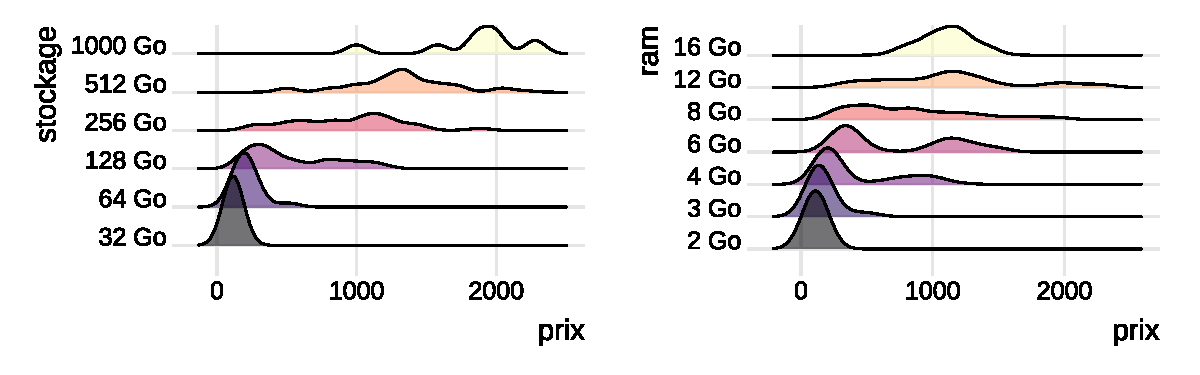
\includegraphics{report_files/figure-pdf/ggplots-1.pdf}

}

\caption{Ridge plot : Stockage et RAM}

\end{figure}%

\newpage

\section{Etudes des variables catégorielles
importantes}\label{etudes-des-variables-catuxe9gorielles-importantes}

Nous allons maintenant étudier les proportions des modalités des
variables catégorielles.

\begin{figure}[H]

{\centering 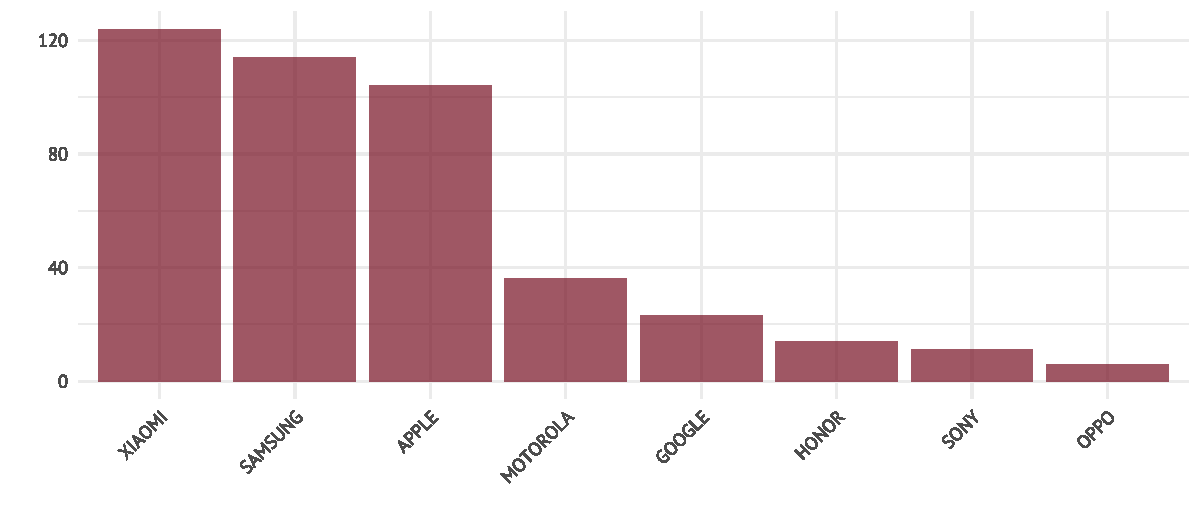
\includegraphics{report_files/figure-pdf/brand_prop-1.pdf}

}

\caption{Proportion des modèles par marque.}

\end{figure}%

\begin{itemize}
\item
  Samsung, Apple \& Xiamoi se partagent 70\% des téléphones
  commercialisés sur Boulanger.
\item
  On retrouve la même tendance au niveau des parts de marché mondial des
  smartphones par rapport à Q3 2022, c'est-à-dire que Samsung, Apple \&
  Xiaomi se partagent respectivement 22, 18 et 14\% de parts de marché.
\end{itemize}

\begin{figure}[H]

{\centering 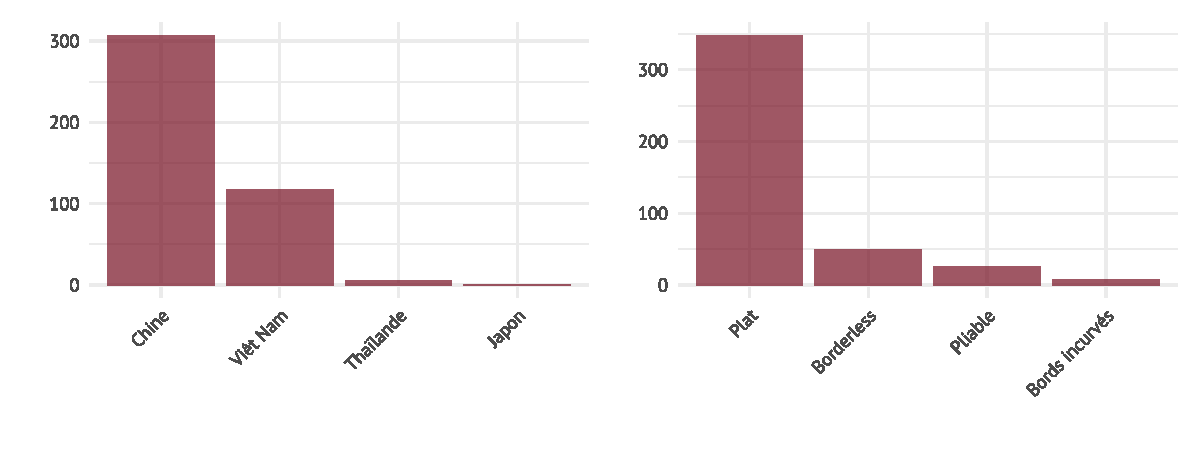
\includegraphics{report_files/figure-pdf/location_prop-1.pdf}

}

\caption{Nombre de smartphones par lieu de fabrication et par type
d'écran.}

\end{figure}%

\begin{itemize}
\item
  On remarque que la majorité des smartphones sont fabriqués en Chine et
  au Viêt Nam (\emph{97.5}\%). Les 12 téléphones restants sont fabriqués
  en Thaïlande, au Japon, en Inde et à Taïwan.
\item
  Concernant les types d'écran, 76.2\% des écrans sont \emph{plats},
  14.6\% sont \emph{borderless} (bord à bord), il y a 7.4\% d'écrans
  pliables et finalement 1.8\% d'écrans à bords incurvés.
\end{itemize}

\newpage

\section{Etude des variables
dichotomiques}\label{etude-des-variables-dichotomiques}

Nos données contiennent 4 variables dichotomiques aux modalités
\texttt{TRUE} ou \texttt{FALSE}.

Ces variables sont :

\begin{itemize}
\tightlist
\item
  \emph{induction} \(\Rightarrow\) le téléphone dispose-t-il d'une
  charge à induction ?
\item
  \emph{fast\_charging} \(\Rightarrow\) le téléphone dispose-t-il d'une
  charge rapide ?
\item
  \emph{upgrade\_storage} \(\Rightarrow\) la capacité de stockage
  est-elle extensible ?
\item
  \emph{usb\_type\_c} \(\Rightarrow\) le téléphone possède-t-il un port
  USB type C ?
\end{itemize}

\begin{figure}[H]

{\centering 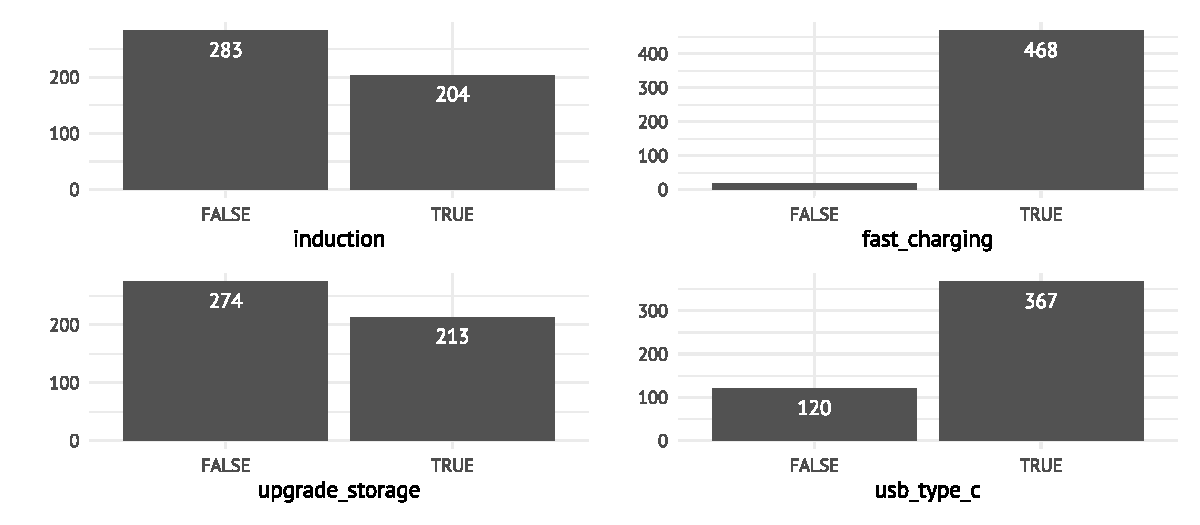
\includegraphics{report_files/figure-pdf/binary_vars-1.pdf}

}

\caption{Proportion de modalités des variables dichotomiques.}

\end{figure}%

Si les modalités sont plutôt bien équilibrées pour les variables
\emph{induction} et \emph{upgrade\_storage}, ce n'est pas le cas pour la
variable \emph{usb\_type\_c} et le déséquilibre est surtout présent pour
\emph{fast\_charging}. En effet seulement 19 téléphones n'ont pas de
charge rapide (ces 19 téléphones sont beaucoup moins chers et sont
principalement des téléphones bas de gamme).

Pour la variable \emph{usb\_type\_c}, il y a 120 téléphones sans
chargeur USB type C et le fait de ne pas avoir d'USB type C fait
augmenter le prix moyen par rapport aux téléphones qui en ont (les
téléphones n'ayant pas d'USB type C sont principalement de marque
\emph{Apple}, ce qui explique en partie l'effet).

Le même effet d'augmentation du prix moyen s'observe avec la variable
\emph{upgrade\_storage}, c'est-à-dire que les téléphones ne possédant
pas de système leur permettant d'augmenter leur stockage sont en moyenne
plus chers que les téléphones offrant la possibilité de le faire. Ce qui
peut paraître à première vue contre-intuitif ne l'est peut-être pas :
les téléphones offrant la possibilité d'augmenter le stockage sont ceux
qui en ont le moins, d'où la nécessité de laisser au consommateur la
possibilité de pouvoir le faire. Inversement, les téléphones qui n'ont
pas de système d'augmentation de stockage ont déjà un stockage
important.

Les téléphones avec charge à induction sont eux en moyenne beaucoup plus
chers que les téléphones ne disposant pas de charge à induction.

\newpage

\section{Analyse des corrélations}\label{analyse-des-corruxe9lations}

Une analyse approfondie des corrélations entre l'ensemble des variables
numériques disponibles va nous permettre de mesurer la force de la
relation linéaire entre paires de variables. Cela nous sera
particulièrement utile pour déterminer les variables explicatives
fortement corrélées à notre variable à prédire \textbf{price}.

\begin{figure}[H]

{\centering 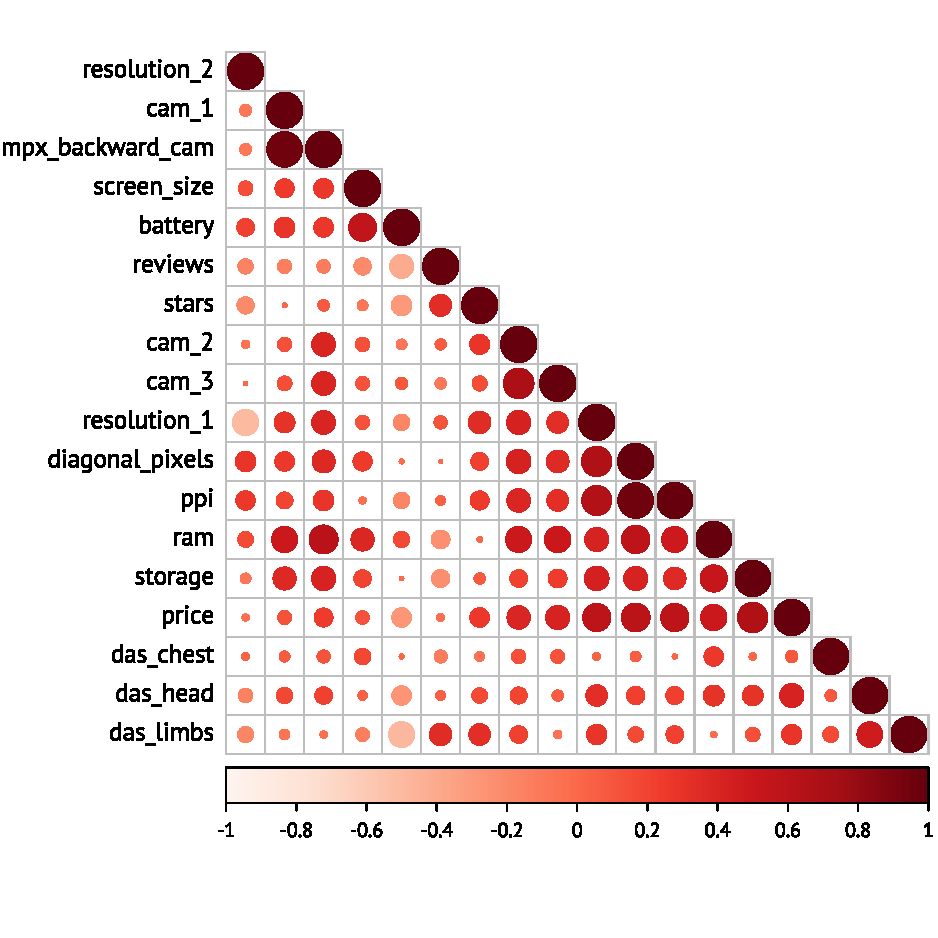
\includegraphics{report_files/figure-pdf/correlation-1.pdf}

}

\caption{Matrice des corrélations.}

\end{figure}%

On s'aperçoit que les corrélations les plus importantes avec
\textbf{price} sont respectivement la capacité de stockage avec un
coefficient de corrélation \(r_{price, storage}=\) 0.73 et la RAM avec
\(r_{price, ram}=\) 0.55. Inversement, la hauteur du téléphone, par
exemple, semble ne pas avoir d'incidence sur le prix avec
\(r_{price, height}=\) 0.002.

\textbf{Compte tenu de la littérature existante et de nos observations,
la RAM et la capacité de stockage sont donc des variables
incontournables dans la modélisation des prix des smartphones.}

\chapter{Modélisation
économétrique}\label{moduxe9lisation-uxe9conomuxe9trique}

\section{Sélection de variables}\label{suxe9lection-de-variables}

Avec 35 variables explicatives, le choix des variables
\emph{essentielles} à retenir est important.

La première question qui se pose, en amont de la modélisation, est celle
de la \textbf{sélection de variables}. En effet, si nous sélectionnons
trop de variables, nous risquons de faire du sur-apprentissage et de
modéliser le bruit au lieu des liens statistiques existants. Le but est
donc de trouver un ensemble optimal de variables.

Traditionnellement en économétrie appliquée, plusieurs approches
heuristiques similaires décrites par Efroymson
(\citeproc{ref-efroymson1960}{1960}) ont été utilisées pour le problème
de la sélection de variables comme la \emph{Backward Elimination} ou la
\emph{Forward Selection}.

Nous allons ici décrire en détail la procédure de \emph{Foward
Selection} :

\begin{enumerate}
\def\labelenumi{\arabic{enumi}.}
\tightlist
\item
  On commence par un modèle \(\mathcal{M}_0\), c'est à dire avec
  constante seulement.
\item
  On ajoute les variables \(X_i\) une à une dans le modèle.
\item
  Parmi ces variables, on retient la variable \textbf{la plus
  significative} dans le modèle.
\item
  On réitère la procédure jusqu'à atteindre un modèle contenant
  uniquement des variables significatives à un seuil spécifié.
\end{enumerate}

\begin{tcolorbox}[enhanced jigsaw, colframe=quarto-callout-warning-color-frame, colbacktitle=quarto-callout-warning-color!10!white, left=2mm, rightrule=.15mm, toprule=.15mm, bottomtitle=1mm, breakable, colback=white, titlerule=0mm, coltitle=black, arc=.35mm, opacitybacktitle=0.6, opacityback=0, bottomrule=.15mm, leftrule=.75mm, toptitle=1mm, title=\textcolor{quarto-callout-warning-color}{\faExclamationTriangle}\hspace{0.5em}{Limites}]

\textbf{Il existe cependant plusieurs problèmes dans ces méthodes.}

\begin{itemize}
\item
  La \emph{Backward Elimination} et la \emph{Foward Selection} ne
  convergent pas tout le temps vers le même modèle.
\item
  Le modèle final n'est pas forcément optimal.
\end{itemize}

\end{tcolorbox}

Pour pallier à ces problèmes, une autre approche possible consiste à
faire une recherche exhaustive, c'est-à-dire explorer l'\emph{ensemble}
des modèles possibles. Bien que ce soit la meilleure méthode pour
obtenir avec certitude le modèle optimal, elle devient rapidement
inadaptée dès qu'il y a un nombre de variables trop conséquent, car le
nombre de combinaisons possibles de modèles explose.

Néanmoins, une dernière approche existe : les \emph{algorithmes
génétiques}. Contrairement à la \emph{forward selection} et la
\emph{backward elimination} qui sont des méthodes déterministes, les
algorithmes génétiques sont eux stochastiques.

\begin{itemize}
\tightlist
\item
  On peut s'intéresser à plusieurs critères comme : le \(R^2\), le
  \(R^2\) ajusté, l'\(AIC\), le \(BIC\), etc.
\end{itemize}

Cet algorithme est implémenté dans le package \faIcon{r-project} de
\texttt{\{glmulti\}}.

\begin{itemize}
\item
  On l'utilise quand le nombre de variables est très important.
\item
  Consiste à générer au hasard une population de modèles candidats pour
  ensuite leur permettre d'évoluer. Cette évolution se déroule de
  génération en génération.
\item
  Permet de trouver le meilleur modèle en explorant seulement un
  sous-ensemble de modèles (de manière aléatoire) mais avec un biais
  vers de meilleurs modèles grâce à la sélection.
\end{itemize}

\newpage

\section{Modèle Hédonique
niveau-niveau}\label{moduxe8le-huxe9donique-niveau-niveau}

Pour la facilité des interprétations, dans cette partie, nous
commencerons par utiliser un modèle \emph{level} \(-\) \emph{level},
donc notre variable à prédire \textbf{price} ne sera pas mise sous forme
logarithmique. Dans une seconde partie, nous préférerons un modèle
\emph{log} \(-\) \emph{level}, qui nous permettra de comparer
directement les coefficients de la régression hédonique des prix avec
les coefficients de la \textbf{SFA}.

Nous allons tout d'abord retirer quelques variables qui ne nous seront
pas utiles pour l'analyse et qui risquent de complexifier les
régressions : \emph{cpu}, \emph{model}, \emph{sensor},
\emph{screen\_tech}, \emph{stars}, \emph{reviews}, \emph{color},
\emph{cam\_1}, \emph{cam\_2}, \emph{cam\_3}. Par exemple, il y a presque
autant de modèles distincts que de nombre d'observations, et
\emph{reviews} et \emph{stars} sont si peu corrélées à la variable à
expliquer \textbf{price} que les ajouter ne semble pas nécessaire.

\begin{table}[!h]
\centering
\caption{\label{tab:kable_perf}Comparaison des méthodes de sélection (1).}
\centering
\begin{tabular}[t]{llrrrrrr}
\toprule
\textbf{Méthode} & \textbf{Modèle} & \textbf{$AIC$} & \textbf{$AIC_{wt}$} & \textbf{$BIC$} & \textbf{$BIC_{wt}$} & \textbf{$R^2_{adj}$} & \textbf{$RMSE$}\\
\midrule
\cellcolor{gray!10}{backward} & \cellcolor{gray!10}{lm} & \cellcolor{gray!10}{6218.90} & \cellcolor{gray!10}{0.72} & \cellcolor{gray!10}{6386.43} & \cellcolor{gray!10}{0} & \cellcolor{gray!10}{0.93} & \cellcolor{gray!10}{132.14}\\
forward & lm & 6220.85 & 0.27 & 6380.00 & 0 & 0.93 & 132.95\\
\cellcolor{gray!10}{genetic} & \cellcolor{gray!10}{lm} & \cellcolor{gray!10}{6229.89} & \cellcolor{gray!10}{0.00} & \cellcolor{gray!10}{6363.91} & \cellcolor{gray!10}{1} & \cellcolor{gray!10}{0.92} & \cellcolor{gray!10}{135.85}\\
\bottomrule
\end{tabular}
\end{table}

\textbf{Quelques commentaires} : On s'aperçoit que la méthode
\emph{backward} et \emph{forward} n'ont pas convergé vers le même modèle
: plus précisément, certaines variables comme \emph{diagonal\_pixels} ou
\emph{battery} ont été sélectionnées dans la \emph{backward} mais pas
dans la \emph{forward} (\textbf{On le pressentait, c'est une limite de
la méthode}). Plus de détail peut être trouvé dans les résultats des
régressions ci-dessous.

On préférera aussi regarder comme critère le \(BIC\) car il est plus
parcimonieux que l'\(AIC\).

\[ BIC = -2\ln(\mathcal{L}) + k \cdot \ln(N) \]

\begin{itemize}
\tightlist
\item
  Avec \(\mathcal{L}\) la vraisemblance du modèle estimée, \(N\) le
  nombre d'observations dans l'échantillon et \(k\) le nombre de
  paramètres libres du modèle.
\end{itemize}

Comparé à l'\(AIC\), il pénalise plus le nombre de variables présentes
dans le modèle. On voit d'ailleurs dans ce tableau que l'algorithme
génétique possède le \(BIC\) le plus bas, tout en ayant un \(R^2_{adj}\)
très légèrement inférieur aux méthodes \emph{backward} et
\emph{forward}. On le verra aussi dans le tableau des résultats de
régression, mais la régression trouvée par l'algorithme génétique
possède moins de variables (12), et celles-ci sont toutes significatives
à un seuil \(p<0.01\).

Le modèle que nous allons étudier ici sera donc :

\begin{equation}\phantomsection\label{eq-level-hedonic}{
\begin{split}
price_i = \beta_0 + \beta_{1i} storage_i + \beta_{2i}brand_i + \beta_{3i}ram_i + \beta_{4i}screen\_type_i \\
+ \beta_{5i}induction_i + \beta_{6i}screen\_size_i + \beta_{7i}repairability\_index_i \\
+ \beta_{8i}made\_in_i + \beta_{9i}upgrade\_storage_i + \beta_{10i}fast\_charging_i  \\
+ \beta_{11i}das\_limbs_i + \beta_{12i}das\_chest_i + \epsilon_i
\end{split}
}\end{equation}

On voit que dans le modèle de l'équation~\ref{eq-level-hedonic}, il n'y
a pour l'instant aucun effet d'interaction ou d'effet non-linéaire. Pour
autant, les résultats sont déjà \textbf{très satisfaisants} avec un
\(R^2_{adj} > 0.9\)

\newpage

\begin{figure}[H]

{\centering 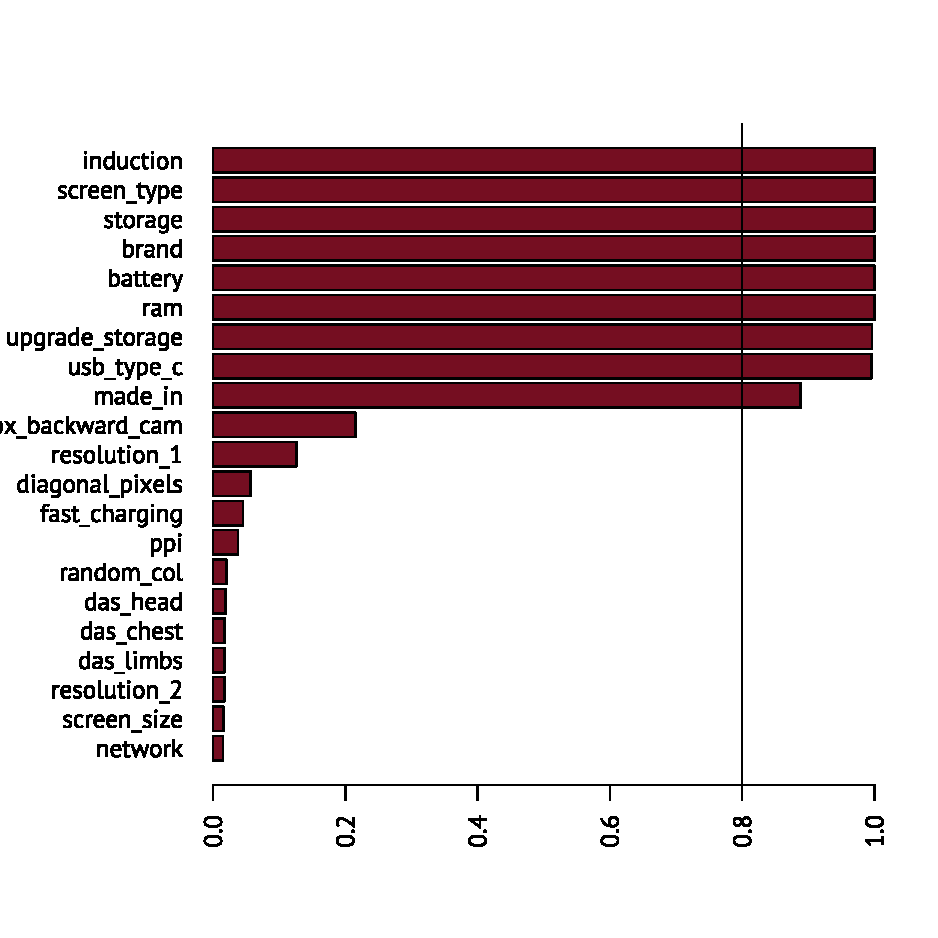
\includegraphics{report_files/figure-pdf/var_importance-1.pdf}

}

\caption{Importance des variables.}

\end{figure}%

L'importance d'une variable, dans ce contexte, est égale à la somme des
probabilités pour les modèles dans lesquels la variable apparaît. Ainsi,
une variable présente dans de nombreux modèles avec des poids importants
recevra une valeur d'importance élevée. La ligne rouge verticale est
tracée à 0.8, correspondant au seuil différenciant les variables
importantes des variables moins importantes, mais ce choix (80\%) est
arbitraire.

Ainsi, on remarque que 11 variables sont présentes dans l'ensemble des
modèles, donc ces variables sont très importantes. Ensuite, une seule
variable est au-dessus de la ligne de \emph{cutoff} mais inférieure à 1
: \emph{das\_head}. L'ensemble des autres variables sont comprises entre
0 et 0.25. On peut donc considérer que l'importance de ces variables
dans notre modèle est négligeable.

\begin{table}[!htbp] \centering 
  \caption{Comparaison des méthodes de sélection (2).} 
  \label{} 
\footnotesize 
\begin{tabular}{@{\extracolsep{5pt}}lccc} 
\\[-1.8ex]\hline 
\hline \\[-1.8ex] 
 & \multicolumn{3}{c}{\textit{Dependent variable:}} \\ 
\cline{2-4} 
\\[-1.8ex] & \multicolumn{3}{c}{price} \\ 
 & forward & backward & genetic \\ 
\\[-1.8ex] & (1) & (2) & (3)\\ 
\hline \\[-1.8ex] 
 storage & 0.749$^{***}$ (0.047) & 0.748$^{***}$ (0.047) & 0.742$^{***}$ (0.047) \\ 
  brandASUS & $-$408.264$^{***}$ (68.796) & $-$414.207$^{***}$ (73.424) & $-$501.156$^{***}$ (58.681) \\ 
  brandFAIRPHONE & $-$596.063$^{***}$ (93.349) & $-$551.526$^{***}$ (93.980) & $-$592.163$^{***}$ (93.040) \\ 
  brandGOOGLE & $-$473.395$^{***}$ (60.739) & $-$464.841$^{***}$ (64.695) & $-$493.572$^{***}$ (52.844) \\ 
  brandHONOR & $-$834.094$^{***}$ (60.479) & $-$808.301$^{***}$ (62.620) & $-$863.679$^{***}$ (57.603) \\ 
  brandMOTOROLA & $-$632.526$^{***}$ (50.179) & $-$606.074$^{***}$ (51.282) & $-$678.762$^{***}$ (39.917) \\ 
  brandNOTHING & $-$832.362$^{***}$ (68.803) & $-$807.903$^{***}$ (68.568) & $-$896.865$^{***}$ (59.170) \\ 
  brandONEPLUS & $-$562.556$^{***}$ (68.355) & $-$549.520$^{***}$ (68.277) & $-$614.648$^{***}$ (61.358) \\ 
  brandOPPO & $-$593.068$^{***}$ (50.540) & $-$576.039$^{***}$ (50.665) & $-$628.747$^{***}$ (45.326) \\ 
  brandREALME & $-$480.079$^{***}$ (52.804) & $-$471.156$^{***}$ (53.481) & $-$469.539$^{***}$ (49.256) \\ 
  brandSAMSUNG & $-$439.536$^{***}$ (58.339) & $-$427.905$^{***}$ (58.337) & $-$501.056$^{***}$ (47.367) \\ 
  brandSONY & $-$467.249$^{***}$ (76.229) & $-$517.148$^{***}$ (78.426) & $-$433.391$^{***}$ (72.424) \\ 
  brandVIVO & $-$577.364$^{***}$ (57.733) & $-$560.288$^{***}$ (57.863) & $-$580.769$^{***}$ (55.456) \\ 
  brandXIAOMI & $-$595.182$^{***}$ (37.741) & $-$585.623$^{***}$ (37.671) & $-$581.323$^{***}$ (35.091) \\ 
  ram & 37.750$^{***}$ (4.407) & 37.089$^{***}$ (4.419) & 42.632$^{***}$ (3.984) \\ 
  resolution\_1 &  & 0.435$^{**}$ (0.169) &  \\ 
  resolution\_2 &  & 0.425$^{**}$ (0.165) &  \\ 
  battery &  & 0.029$^{*}$ (0.017) &  \\ 
  screen\_typeBords incurvés & $-$192.989$^{***}$ (70.750) & $-$173.485$^{**}$ (69.119) & $-$147.108$^{**}$ (67.210) \\ 
  screen\_typePlat & $-$123.016$^{***}$ (30.006) & $-$115.179$^{***}$ (31.347) & $-$100.500$^{***}$ (27.764) \\ 
  screen\_typePliable & 304.117$^{***}$ (44.035) & 300.618$^{***}$ (47.009) & 316.851$^{***}$ (43.490) \\ 
  induction & 168.220$^{***}$ (23.570) & 174.465$^{***}$ (23.639) & 156.811$^{***}$ (23.219) \\ 
  screen\_size & 167.430$^{***}$ (22.390) & 113.845$^{***}$ (22.974) & 154.687$^{***}$ (18.536) \\ 
  repairability\_index & 96.173$^{***}$ (13.963) & 92.514$^{***}$ (14.347) & 108.973$^{***}$ (13.539) \\ 
  diagonal\_pixels &  & $-$0.540$^{**}$ (0.221) &  \\ 
  made\_inInde & $-$114.552 (147.903) & $-$90.982 (147.403) & $-$21.635 (144.976) \\ 
  made\_inJapon & 562.032$^{***}$ (122.398) & 575.013$^{***}$ (122.145) & 562.520$^{***}$ (123.872) \\ 
  made\_inTaïwan & 364.924$^{**}$ (146.439) & 371.614$^{**}$ (147.234) & 376.405$^{**}$ (148.161) \\ 
  made\_inThaïlande & 520.712$^{***}$ (84.016) & 530.761$^{***}$ (83.910) & 540.906$^{***}$ (83.742) \\ 
  made\_inViêt Nam & $-$42.481 (40.358) & $-$46.251 (40.181) & $-$27.599 (39.736) \\ 
  upgrade\_storage & $-$121.057$^{***}$ (26.861) & $-$141.890$^{***}$ (27.060) & $-$133.052$^{***}$ (25.669) \\ 
  fast\_charging & $-$159.191$^{***}$ (37.214) & $-$135.971$^{***}$ (37.830) & $-$145.993$^{***}$ (36.887) \\ 
  das\_limbs & 87.183$^{***}$ (19.892) & 86.927$^{***}$ (20.274) & 72.879$^{***}$ (18.845) \\ 
  das\_head & $-$122.268$^{***}$ (37.963) & $-$137.406$^{***}$ (38.904) & $-$105.158$^{***}$ (38.084) \\ 
  das\_chest & $-$150.742$^{**}$ (59.690) & $-$142.616$^{**}$ (60.016) &  \\ 
  mpx\_backward\_cam & 0.334 (0.243) &  &  \\ 
  random\_col & $-$0.018 (0.012) & $-$0.017 (0.012) &  \\ 
  usb\_type\_c & 39.228$^{*}$ (22.151) & 42.748$^{*}$ (21.936) &  \\ 
  height & $-$0.306$^{*}$ (0.156) & $-$0.331$^{**}$ (0.158) &  \\ 
  ppi & 0.170 (0.114) &  &  \\ 
  Constant & $-$924.262$^{***}$ (195.491) & $-$697.920$^{***}$ (174.947) & $-$1,050.746$^{***}$ (155.543) \\ 
 \hline \\[-1.8ex] 
Observations & 487 & 487 & 487 \\ 
R$^{2}$ & 0.931 & 0.932 & 0.928 \\ 
Adjusted R$^{2}$ & 0.925 & 0.926 & 0.923 \\ 
Residual Std. Error & 138.303 (df = 450) & 137.768 (df = 448) & 140.390 (df = 456) \\ 
F Statistic & 168.461$^{***}$ (df = 36; 450) & 160.983$^{***}$ (df = 38; 448) & 195.544$^{***}$ (df = 30; 456) \\ 
\hline 
\hline \\[-1.8ex] 
\textit{Note:}  & \multicolumn{3}{r}{$^{*}$p$<$0.1; $^{**}$p$<$0.05; $^{***}$p$<$0.01} \\ 
\end{tabular} 
\end{table}

\newpage

\subsection{Interpétations Modèle
niveau-niveau}\label{interpuxe9tations-moduxe8le-niveau-niveau}

\begin{itemize}
\item
  Si la capacité de stockage (\emph{storage}) augmente de 1 Go, alors,
  le prix augmente de 0.74 €, \emph{cet. par.}
\item
  En ayant comme catégorie de référence \emph{Apple} pour la variable
  marque (\emph{brand}), on peut voir que toutes les marques ont un
  impact négatif sur le prix, \emph{cet. par.}

  \begin{itemize}
  \tightlist
  \item
    La marque la plus valorisée derrière \emph{Apple} est \emph{Sony}
    avec 433.39 € de différence par rapport à \emph{Apple}.
  \item
    La marque la moins valorisée est \emph{Nothing} avec 896.87 € de
    différence par rapport à \emph{Apple}
  \end{itemize}
\item
  Une augmentation d'un Go de \emph{ram} augmente le prix de 42.63 €,
  \emph{cet. par.}
\item
  Pour le type d'écran (\emph{screen\_type}), la catégorie de référence
  est \emph{borderless} (un écran sans bordure).

  \begin{itemize}
  \tightlist
  \item
    Disposer d'un écran à bord incurvé diminue le prix de 147.11 € par
    rapport à la catégorie de référence, \emph{cet. par.}
  \item
    Pour l'écran plat, le prix diminue de 100.5 € par rapport à la
    catégorie de référence, \emph{cet. par.}
  \item
    Avoir un écran pliable fait augmenter le prix de 316.85 € par
    rapport à la catégorie de référence, \emph{cet. par.}
  \end{itemize}
\item
  Posséder un dispositif de charge à induction (\emph{induction =
  \texttt{TRUE}}) augmente le prix de 156.81 €, \emph{cet. par.}
\item
  Si la taille de l'écran augmente de 1 pouce, alors le prix augmente de
  154.69 €, \emph{cet. par.}
\item
  L'indice de réparabilité (\emph{repairability\_index}) est compris
  entre 1 et 10. Une augmentation de 1 point de cet indice implique une
  augmentation de 108.97 €, \emph{cet. par.}
\item
  Concernant le lieu de fabrication (\emph{made\_in}), la catégorie de
  référence est la \emph{Chine}.

  \begin{itemize}
  \tightlist
  \item
    Les coefficients associés aux catégories \emph{Inde} et \emph{Viêt
    Nam} ne sont pas significatives, c'est-à-dire qu'il n'y a pas de
    différence significative de prix avec un smartphone produit en
    \emph{Chine}.
  \item
    Comparé à un téléphone fabriqué en Chine, un téléphone produit au
    \emph{Japon} augmente le prix de 562.52 €, suivi de la
    \emph{Thaïlande} avec une augmentation de 540.91 € et enfin de
    \emph{Taïwan} avec une augmentation du prix de 376.4 €, \emph{cet.
    par.}
  \end{itemize}
\item
  Si le téléphone dispose d'un moyen d'augmenter sa capacité de stockage
  (\emph{upgrade\_storage} = \texttt{TRUE}\emph{), alors le prix diminue
  de 133.05 €,} cet. par.* Comme nous l'avions remarqué dans la partie
  de statistiques descriptives.
\item
  Si le téléphone dispose d'une charge rapide (\emph{fast\_charging =
  \texttt{TRUE}}), alors le prix diminue de 145.99 €, \emph{cet.par.}
\item
  Pour les variables liées au DAS, l'effet de \emph{das\_limbs} est
  positif sur le prix, tandis que l'effet de \emph{das\_head} est quant
  à lui négatif. L'augmentation d'une unité de Watts par kilogramme du
  \emph{das\_limbs} augmente le prix de 72.88 € alors que cette même
  augmentation diminue le prix de 105.16 € pour \emph{das\_head},
  \emph{cet.par.} Néanmoins, l'effet peut être globalement vu comme
  négatif étant donné la valeur des coefficients.
\end{itemize}

\(R^2_{adj} = 0.923\) donc 92.3\% de la variance de la variable
expliquée (price) est expliquée par la variance des variables
explicatives du modèle.

\newpage

\section{Modèle Hédonique
log-niveau}\label{moduxe8le-huxe9donique-log-niveau}

Dans cette partie, nous n'effectuerons pas de sélection de variables
avec \texttt{\{glmulti\}} car le meilleur modèle de régression hédonique
proposé en \emph{log} \(-\) \emph{level} aboutit à des difficultés de
convergence pour le modèle \textbf{SFA}. Or, nous voulons comparer les
coefficients de cette régression hédonique avec les modèles SFA que nous
mettrons en place dans une troisième phase.

\begin{tcolorbox}[enhanced jigsaw, colframe=quarto-callout-warning-color-frame, colbacktitle=quarto-callout-warning-color!10!white, left=2mm, rightrule=.15mm, toprule=.15mm, bottomtitle=1mm, breakable, colback=white, titlerule=0mm, coltitle=black, arc=.35mm, opacitybacktitle=0.6, opacityback=0, bottomrule=.15mm, leftrule=.75mm, toptitle=1mm, title=\textcolor{quarto-callout-warning-color}{\faExclamationTriangle}\hspace{0.5em}{Difficultés de convergence d'un modèle SFA}]

Dans une \textbf{SFA}, les difficultés de convergence peuvent être dues
à de vastes zones très plates de la fonction de vraisemblance, pouvant
être causées par une forte multicolinéarité entre l'intercept du modèle
de frontière et l'intercept du modèle d'inefficacité. Par conséquent,
supprimer l'intercept du modèle d'inefficacité améliore parfois la
convergence, mais risque aussi d'introduire un biais de variable omise.

\vspace{1em}

Dans le package \texttt{\{frontier\}} que nous utilisons pour effectuer
la SFA, ces difficultés sont en général indiquées par le message
d'avertissement suivant :

\vspace{1em}

\begin{itemize}
\tightlist
\item
  \emph{``le paramètre gamma est proche de la limite de l'espace des
  paramètres {[}0,1{]}''}
\end{itemize}

\vspace{1em}

Cela signifie que l'estimation du paramètre \(\gamma\) est soit proche
de la limite inférieure de son espace de paramètres (0), soit proche de
la limite supérieure de son espace de paramètres (1). Par exemple, un
\(\gamma\) proche de zéro indique qu'il n'y a presque aucune
inefficacité, donc qu'il serait possible d'estimer le modèle par MCO,
tandis qu'un \(\gamma\) proche de un indique qu'il n'y a presque aucun
bruit, donc qu'il serait possible d'utiliser une DEA. Plus globalement,
cela indique une mauvaise spécification du modèle ou que d'autres
modèles pourraient être plus appropriés dans ce cadre.

\end{tcolorbox}

Après plusieurs essais, le modèle que nous avons choisi d'étudier est :

\begin{equation}\phantomsection\label{eq-log-hedonic}{
\begin{split}
\ln(price_i) = \beta_0 + \beta_{1i} storage_i + \beta_{2i}brand_i + \beta_{3i}ram_i + \beta_{4i}induction_i \\
+ \beta_{5i}screen\_size_i + \beta_{6i}made\_in_i + \beta_{7i}upgrade\_storage_i \\
+ \beta_{8i}das\_head_i + \beta_{9i}das\_limbs_i + \beta_{10i}das\_chest_i  \\
+ \beta_{11i}fast\_charging_i + \beta_{12i}network_i + \beta_{13i}ppi_i + \epsilon_i
\end{split}
}\end{equation}

Par rapport au modèle en niveau, il n'y a plus les variables
\emph{screen\_type} et \emph{repairability\_index}, qui posaient des
problèmes de convergence. D'autres variables ont néanmoins été
introduites comme \emph{network} ou \emph{ppi}.

\begin{center}\rule{0.5\linewidth}{0.5pt}\end{center}

\begin{table}[!htbp] \centering 
  \caption{Modèle de Pricing Hédonique Log-Linéaire } 
  \label{} 
\footnotesize 
\begin{tabular}{@{\extracolsep{5pt}}lc} 
\\[-1.8ex]\hline 
\hline \\[-1.8ex] 
 & \multicolumn{1}{c}{\textit{Dependent variable:}} \\ 
\cline{2-2} 
\\[-1.8ex] & logprice \\ 
\hline \\[-1.8ex] 
 storage & 0.001$^{***}$ (0.0001) \\ 
  brandASUS & $-$0.357$^{***}$ (0.109) \\ 
  brandFAIRPHONE & $-$0.179 (0.140) \\ 
  brandGOOGLE & $-$0.430$^{***}$ (0.090) \\ 
  brandHONOR & $-$0.987$^{***}$ (0.080) \\ 
  brandMOTOROLA & $-$0.718$^{***}$ (0.073) \\ 
  brandNOTHING & $-$0.877$^{***}$ (0.107) \\ 
  brandONEPLUS & $-$0.652$^{***}$ (0.107) \\ 
  brandOPPO & $-$0.664$^{***}$ (0.077) \\ 
  brandREALME & $-$0.644$^{***}$ (0.080) \\ 
  brandSAMSUNG & $-$0.151$^{*}$ (0.085) \\ 
  brandSONY & $-$0.356$^{***}$ (0.115) \\ 
  brandVIVO & $-$0.589$^{***}$ (0.088) \\ 
  brandXIAOMI & $-$0.759$^{***}$ (0.056) \\ 
  ram & 0.082$^{***}$ (0.007) \\ 
  induction & 0.272$^{***}$ (0.037) \\ 
  screen\_size & 0.241$^{***}$ (0.033) \\ 
  made\_inInde & $-$0.225 (0.233) \\ 
  made\_inJapon & 0.414$^{**}$ (0.189) \\ 
  made\_inTaïwan & 0.475$^{**}$ (0.234) \\ 
  made\_inThaïlande & 0.543$^{***}$ (0.134) \\ 
  made\_inViêt Nam & $-$0.149$^{***}$ (0.053) \\ 
  upgrade\_storage & $-$0.363$^{***}$ (0.039) \\ 
  das\_head & $-$0.209$^{***}$ (0.061) \\ 
  das\_limbs & 0.092$^{***}$ (0.030) \\ 
  das\_chest & $-$0.299$^{***}$ (0.095) \\ 
  fast\_charging & $-$0.138$^{**}$ (0.058) \\ 
  network5G & 0.306$^{***}$ (0.037) \\ 
  ppi & 0.001$^{***}$ (0.0002) \\ 
  Constant & 4.320$^{***}$ (0.253) \\ 
 \hline \\[-1.8ex] 
Observations & 487 \\ 
R$^{2}$ & 0.933 \\ 
Adjusted R$^{2}$ & 0.929 \\ 
Residual Std. Error & 0.221 (df = 457) \\ 
F Statistic & 219.790$^{***}$ (df = 29; 457) \\ 
\hline 
\hline \\[-1.8ex] 
\textit{Note:}  & \multicolumn{1}{r}{$^{*}$p$<$0.1; $^{**}$p$<$0.05; $^{***}$p$<$0.01} \\ 
\end{tabular} 
\end{table}

\newpage

\subsection{Interpétations Modèle
log-niveau}\label{interpuxe9tations-moduxe8le-log-niveau}

\begin{itemize}
\item
  Si la capacité de stockage (\emph{storage}) augmente de 1 Go, alors le
  prix augmente de 0.1\%, \emph{cet. par.}
\item
  En ayant comme catégorie de référence \emph{Apple} pour la variable
  marque (\emph{brand}), on peut voir que toutes les marques ont un
  impact négatif sur le prix, \emph{cet. par.}

  \begin{itemize}
  \tightlist
  \item
    La marque la plus valorisée derrière \emph{Apple} est \emph{Samsung}
    avec une différence de prix de \(15.1\%\).
  \item
    La marque la moins valorisée est \emph{Honor} avec une différence de
    prix de \(98.7\%\) par rapport à \emph{Apple}.
  \end{itemize}
\item
  Si la \emph{ram} augmente de 1 Go, alors le prix augmente de
  \(8.2\%\), \emph{cet. par.}
\item
  Si le téléphone dispose d'une charge à induction (\emph{induction =
  \texttt{TRUE}}), alors le prix augmente de \(27.2\%\), \emph{cet.
  par.}
\item
  Si la taille de l'écran augmente de 1 pouce (\emph{screen\_size}),
  alors le prix augmente de \(24.1\%\), \emph{cet. par.}
\item
  Pour le lieu de fabrication (\emph{made\_in}), la catégorie de
  référence est la \emph{Chine}.

  \begin{itemize}
  \tightlist
  \item
    Le coefficient associé à la catégorie \emph{Inde} n'est pas
    significatif.
  \item
    Un téléphone qui est fabriqué au \emph{Viêt Nam} est \(14.9\%\)
    moins cher qu'un téléphone fabriqué en \emph{Chine}, \emph{cet.
    par.}
  \item
    Comparé à un téléphone produit en \emph{Chine}, un téléphone produit
    en \emph{Thaïlande} augmente le prix de \(54.3\%\), suivi de
    \emph{Taïwan} avec une augmentation de \(47.5\%\) et enfin du
    \emph{Japon} avec une augmentation du prix de \(41.4\%\), \emph{cet.
    par.}
  \end{itemize}
\item
  Si le téléphone dispose d'un moyen d'augmenter sa capacité de stockage
  (\emph{upgrade\_storage = \texttt{TRUE}}), alors le prix diminue de
  \(36.3\%\), \emph{cet. par}.
\item
  Pour les variables liées au DAS :

  \begin{itemize}
  \tightlist
  \item
    l'augmentation d'une unité de Watts par kilogramme du
    \emph{das\_limbs} augmente le prix de \(9.2\%\), \emph{cet. par.}
  \item
    au contraire, le prix diminue de \(20.9\%\) pour le \emph{das\_head}
    et de \(29.9\%\) pour le \emph{das\_chest} lorsque qu'ils augmentent
    d'une unité de W/kg, \emph{cet. par.}
  \end{itemize}
\item
  Si le téléphone dispose d'une charge rapide (\emph{fast\_charging =
  \texttt{TRUE}}), alors le prix diminue de \(13.9\%\), \emph{cet.par.}
\item
  Si le téléphone est compatible avec la 5G (\emph{network5G =
  \texttt{TRUE}}), alors le prix augmente de \(30.6\%\), \emph{cet.
  par.}
\item
  Lorsque le \emph{ppi} (\emph{pixels par pouce}) augmente d'une unité,
  alors le prix augmente de \(0.1\%\), \emph{cet. par.}
\end{itemize}

\(R^2_{adj} = 0.929\) donc 92.9\% de la variance de la variable
expliquée est expliquée par la variance des variables explicatives du
modèle.

\newpage

\subsection{Vérification des
hypothèses}\label{vuxe9rification-des-hypothuxe8ses}

Un aspect crucial lors de la construction des modèles de régression
linéaire est d'évaluer la qualité de l'ajustement du modèle, mais aussi
de vérifier certaines hypothèses comme :

\begin{enumerate}
\def\labelenumi{\arabic{enumi}.}
\tightlist
\item
  La linéarité dans les paramètres.
\item
  Des résidus d'espérance nulle.
\item
  L'absence de multicolinéarité.
\item
  L'homoscédasticité des résidus.
\end{enumerate}

Pour ce faire, on peut utiliser les packages \texttt{\{performance\}} et
\texttt{\{see\}} en conjonction\footnote{Plus d'infos sur les packages :
  \href{https://easystats.github.io/see/articles/performance.html}{\texttt{see}}
  et
  \href{https://easystats.github.io/performance/index.html}{\texttt{performance}}}.

L'hypothèse \textbf{(1)} est vérifiée par la formulation de notre
modèle. Pour l'hypothèse \textbf{(2)}, on peut effectuer un test de
\emph{Student} pour vérifier si \(E(\epsilon_i) = 0\). Les hypothèses
\(H_0\) et \(H_1\) sont les suivantes :

\[
\begin{cases}
H_0 : E(\epsilon_i) = 0\\
H_1 : E(\epsilon_i) \neq 0
\end{cases}
\]

\vspace{1em}

\begin{itemize}
\tightlist
\item
  La \(p-value\) issue du test est égale à 1, donc l'hypothèse
  \textbf{(2)} est vérifiée.
\end{itemize}

\begin{table}[!h]
\centering
\caption{\label{tab:collinearity}Vérification de la multicolinéarité.}
\centering
\begin{tabular}[t]{lrrrr}
\toprule
\textbf{Variable} & \textbf{VIF} & \textbf{IC \{low\}} & \textbf{IC \{high\}} & \textbf{Tolérance}\\
\midrule
\cellcolor{gray!10}{storage} & \cellcolor{gray!10}{1.99} & \cellcolor{gray!10}{1.77} & \cellcolor{gray!10}{2.27} & \cellcolor{gray!10}{0.50}\\
brand & 470.82 & 398.96 & 555.65 & 0.00\\
\cellcolor{gray!10}{ram} & \cellcolor{gray!10}{4.28} & \cellcolor{gray!10}{3.71} & \cellcolor{gray!10}{4.98} & \cellcolor{gray!10}{0.23}\\
induction & 3.23 & 2.82 & 3.74 & 0.31\\
\cellcolor{gray!10}{screen\_size} & \cellcolor{gray!10}{1.95} & \cellcolor{gray!10}{1.73} & \cellcolor{gray!10}{2.22} & \cellcolor{gray!10}{0.51}\\
\addlinespace
made\_in & 20.32 & 17.30 & 23.90 & 0.05\\
\cellcolor{gray!10}{upgrade\_storage} & \cellcolor{gray!10}{3.72} & \cellcolor{gray!10}{3.23} & \cellcolor{gray!10}{4.31} & \cellcolor{gray!10}{0.27}\\
das\_head & 1.96 & 1.74 & 2.23 & 0.51\\
\cellcolor{gray!10}{das\_limbs} & \cellcolor{gray!10}{2.53} & \cellcolor{gray!10}{2.23} & \cellcolor{gray!10}{2.91} & \cellcolor{gray!10}{0.40}\\
das\_chest & 4.81 & 4.16 & 5.60 & 0.21\\
\addlinespace
\cellcolor{gray!10}{fast\_charging} & \cellcolor{gray!10}{1.27} & \cellcolor{gray!10}{1.17} & \cellcolor{gray!10}{1.43} & \cellcolor{gray!10}{0.79}\\
network & 2.30 & 2.04 & 2.64 & 0.43\\
\cellcolor{gray!10}{ppi} & \cellcolor{gray!10}{2.35} & \cellcolor{gray!10}{2.08} & \cellcolor{gray!10}{2.70} & \cellcolor{gray!10}{0.42}\\
\bottomrule
\end{tabular}
\end{table}

\begin{itemize}
\tightlist
\item
  \emph{Note} : La \textbf{Tolérance} correspond à
  \(\dfrac{1}{\text{VIF}}\), c'est-à-dire que plus le \emph{VIF} sera
  élevé, et plus la \textbf{Tolérance} sera proche de 0.
\end{itemize}

\newpage

\begin{tcolorbox}[enhanced jigsaw, colframe=quarto-callout-tip-color-frame, colbacktitle=quarto-callout-tip-color!10!white, left=2mm, rightrule=.15mm, toprule=.15mm, bottomtitle=1mm, breakable, colback=white, titlerule=0mm, coltitle=black, arc=.35mm, opacitybacktitle=0.6, opacityback=0, bottomrule=.15mm, leftrule=.75mm, toptitle=1mm, title=\textcolor{quarto-callout-tip-color}{\faLightbulb}\hspace{0.5em}{Mesure de la multicolinéarité}]

Le Variance Inflation Factor (\emph{VIF}) est une mesure permettant
d'analyser l'ampleur de la multicolinéarité des termes du modèle. Plus
précisément :

\vspace{1em}

\begin{itemize}
\tightlist
\item
  Un \emph{VIF} inférieur à 5 indique une faible corrélation de ce
  prédicteur avec d'autres prédicteurs.
\item
  Une valeur comprise entre 5 et 10 indique une corrélation modérée.
\item
  Enfin, des valeurs de \emph{VIF} supérieures à 10 sont le signe d'une
  corrélation très élevée.
\end{itemize}

\vspace{1em}

Ce que le VIF apporte en plus d'une simple analyse des corrélations est
l'analyse d'un cas où une variable est fortement corrélée à une
combinaison linéaire de plusieurs variables.

\end{tcolorbox}

Avec un \emph{VIF} estimé de 470.82, il n'est pas surprenant de
constater que la marque est extrêmement corrélée à une combinaison
linéaire de plusieurs variables. On peut par exemple penser au choix de
localisation de la production, le fait de disposer ou non d'un port USB
type C, etc. L'hypothèse \textbf{(3)} n'est donc pas vérifiée, mais cela
est cohérent dans le cadre du modèle.

\begin{center}\rule{0.5\linewidth}{0.5pt}\end{center}

Concernant l'hypothèse \textbf{(4)} - l'Homoscédasticité pour les
modèles de régression linéaire signifie que les résidus du modèle ont
une variance constante. Si cette hypothèse n'est pas respectée, alors
les \emph{erreurs-types} et les \(p-values\) du modèle ne sont plus
fiables. On peut par exemple détecter la présente d'hétéroscédasticité
graphiquement :

\begin{figure}[H]

{\centering 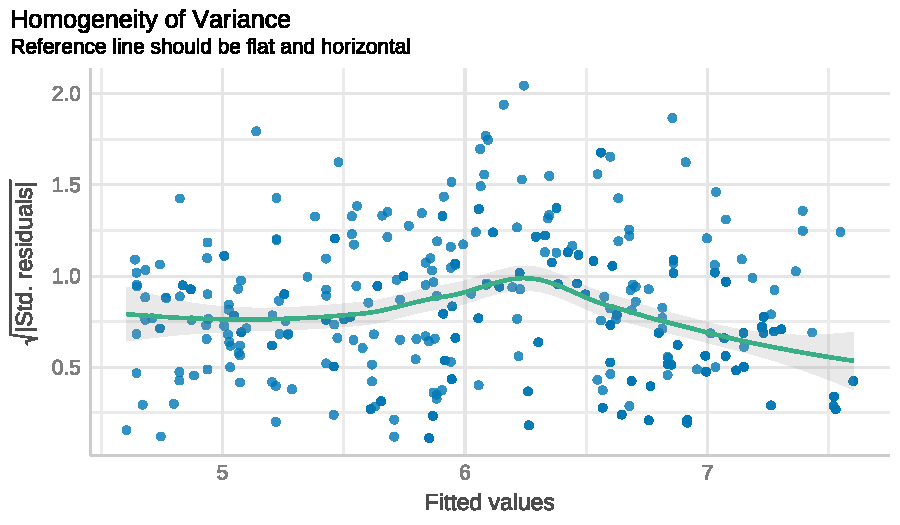
\includegraphics{report_files/figure-pdf/heteroscedasticity-1.pdf}

}

\caption{Homoscédasticité des résidus.}

\end{figure}%

\begin{itemize}
\tightlist
\item
  Il est clair que notre modèle présente des résidus hétéroscédastiques.
  On peut aussi le vérifier avec le test de \emph{Breusch-Pagan}. Les
  hypothèses \(H_0\) et \(H_1\) sont les suivantes :
\end{itemize}

\[
\begin{cases}
H_0 : V(\epsilon_i) = \sigma^2\\
H_1 : V(\epsilon_i) = \sigma^2_i
\end{cases}
\]

\vspace{1em}

\begin{itemize}
\tightlist
\item
  La \(p-value\) issue du test est égale à 0, donc l'hypothèse
  \textbf{(4)} n'est pas vérifiée.
\end{itemize}

\textbf{Il existe néanmoins plusieurs façons de corriger le problème
d'hétéroscédasticité que nous verrons dans la section suivante.}

En complément, on peut aussi tester la normalité des résidus, et
vérifier si certaines observations ont une influence très importante.

\begin{figure}[H]

{\centering 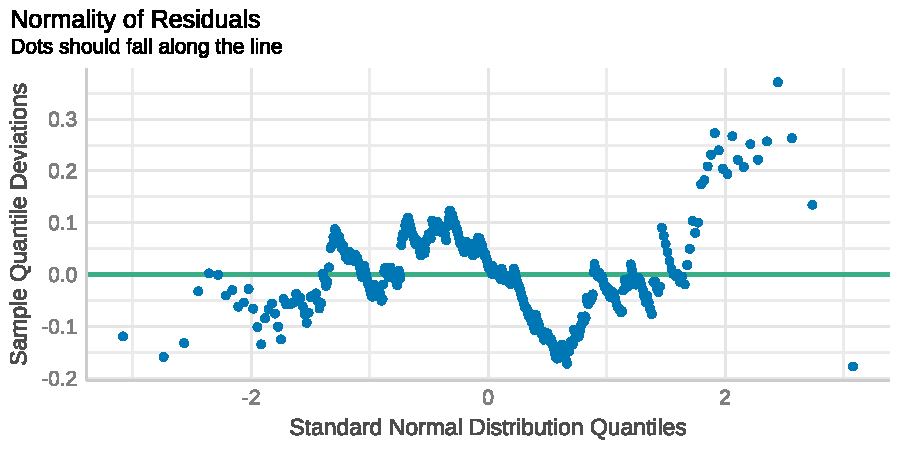
\includegraphics{report_files/figure-pdf/normality-1.pdf}

}

\caption{Normalité des résidus (QQ Plot).}

\end{figure}%

\begin{figure}[H]

{\centering 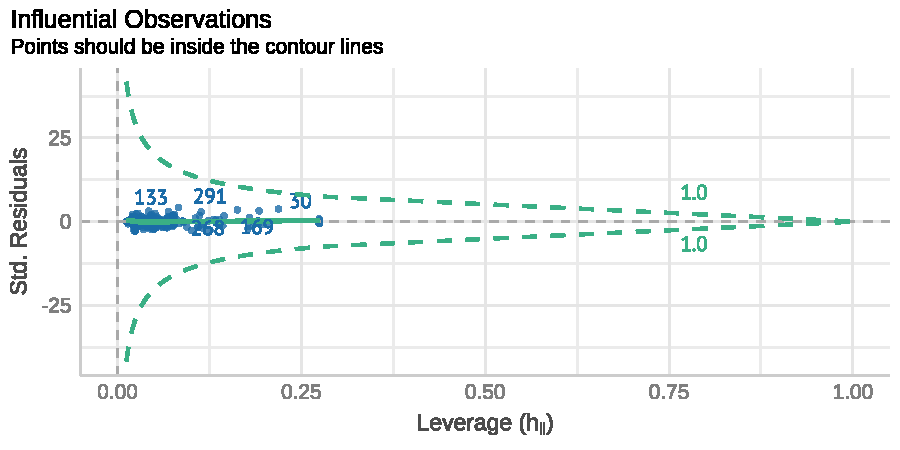
\includegraphics{report_files/figure-pdf/outliers-1.pdf}

}

\caption{Influence des valeurs extrêmes.}

\end{figure}%

\begin{itemize}
\tightlist
\item
  Les résidus ne suivent pas une loi normale et les \emph{outliers}
  n'influent pas sur les résultats des prédictions.
\end{itemize}

\newpage

Enfin, on peut aussi mettre en œuvre une vérification visuelle de
l'ajustement du modèle, en plus des métriques couramment utilisées. La
vérification prédictive a posteriori permet de simuler des données
répliquées avec le modèle ajusté puis les comparer aux données
observées.

\(\Rightarrow\) \textbf{L'objectif est de détecter si le modèle est
inadéquat pour décrire les données.}

\emph{Note} : Les données utilisées pour la vérification prédictive
postérieure sont simulées à partir de la \emph{distribution prédictive
postérieure}. Celle-ci est construite après avoir utilisé les données
observées \(y\) et les prédicteurs \(X\) pour mettre à jour les
croyances sur les paramètres inconnus \(\theta\) dans le modèle. Pour
chaque tirage des paramètres \(\theta\) à partir de la distribution a
posteriori \(p(\theta|y,X)\), un vecteur complet de résultats est
généré.

\begin{center}
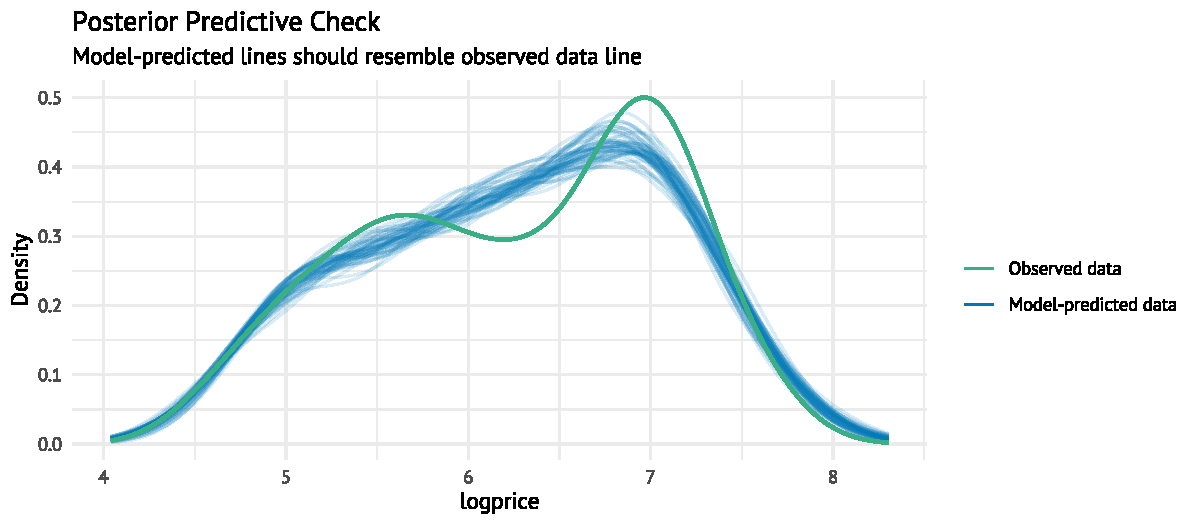
\includegraphics{report_files/figure-pdf/posterior-1.pdf}
\end{center}

\begin{itemize}
\tightlist
\item
  La distribution des prix est bimodale, mais le modèle a du mal à
  représenter le second pic de la distribution. Cependant, les
  prédictions sont assez proches de la réalité.
\end{itemize}

\section{Modèle SFA - Frontière de
coût}\label{moduxe8le-sfa---frontiuxe8re-de-couxfbt}

Le modèle reste le même que celui de l'équation~\ref{eq-log-hedonic},
mais le terme d'erreur \(\epsilon_i\) devient un terme d'erreur composé
\(u_i + v_i\). Pour modéliser cette frontière de coût, il suffit
d'utiliser l'argument \texttt{ineffDecrease\ =\ FALSE}, autrement dit
l'inefficacité augmente la variable endogène.

Il faut maintenant sélectionner la distribution des \(u_i\). Deux
distributions sont disponibles dans le package \texttt{\{frontier\}}:

\begin{itemize}
\tightlist
\item
  La distribution normale tronquée : \texttt{truncNorm\ =\ TRUE}.
\item
  La distribution semi-normale : \texttt{truncNorm\ =\ FALSE}.
\end{itemize}

Nous avons décidé de choisir la distribution *semi-normale.\\
\begin{equation}\phantomsection\label{eq-sfa-cost}{
\begin{split}
\ln(price_i) = \beta_0 + \beta_{1i} storage_i + \beta_{2i}brand_i + \beta_{3i}ram_i + \beta_{4i}induction_i \\
+ \beta_{5i}screen\_size_i + \beta_{6i}made\_in_i + \beta_{7i}upgrade\_storage_i \\
+ \beta_{8i}das\_head_i + \beta_{9i}das\_limbs_i + \beta_{10i}das\_chest_i  \\
+ \beta_{11i}fast\_charging_i + \beta_{12i}network_i + \beta_{13i}ppi_i + \underbrace{\epsilon_i}_{u_i + v_i}
\end{split}
}\end{equation}

\newpage

\begin{table}[!h]
\centering
\caption{\label{tab:scf_results}Résultats de l'estimation du modèle SFA (Cost Frontier).}
\centering
\begin{tabular}[t]{llll}
\toprule
\textbf{ } & \textbf{Coefficient} & \textbf{Significativité} & \textbf{Erreur Std}\\
\midrule
\cellcolor{gray!10}{(Intercept)} & \cellcolor{gray!10}{4.0863} & \cellcolor{gray!10}{***} & \cellcolor{gray!10}{0.2543}\\
storage & 0.0005 & *** & 0.0001\\
\cellcolor{gray!10}{brandASUS} & \cellcolor{gray!10}{-0.3849} & \cellcolor{gray!10}{***} & \cellcolor{gray!10}{0.1092}\\
brandFAIRPHONE & -0.1869 &  & 0.1325\\
\cellcolor{gray!10}{brandGOOGLE} & \cellcolor{gray!10}{-0.5019} & \cellcolor{gray!10}{***} & \cellcolor{gray!10}{0.099}\\
\addlinespace
brandHONOR & -1.0205 & *** & 0.0813\\
\cellcolor{gray!10}{brandMOTOROLA} & \cellcolor{gray!10}{-0.7885} & \cellcolor{gray!10}{***} & \cellcolor{gray!10}{0.0863}\\
brandNOTHING & -0.8851 & *** & 0.1017\\
\cellcolor{gray!10}{brandONEPLUS} & \cellcolor{gray!10}{-0.6815} & \cellcolor{gray!10}{***} & \cellcolor{gray!10}{0.1044}\\
brandOPPO & -0.7405 & *** & 0.091\\
\addlinespace
\cellcolor{gray!10}{brandREALME} & \cellcolor{gray!10}{-0.6727} & \cellcolor{gray!10}{***} & \cellcolor{gray!10}{0.0798}\\
brandSAMSUNG & -0.2256 & * & 0.0957\\
\cellcolor{gray!10}{brandSONY} & \cellcolor{gray!10}{-0.3962} & \cellcolor{gray!10}{***} & \cellcolor{gray!10}{0.1146}\\
brandVIVO & -0.6168 & *** & 0.0872\\
\cellcolor{gray!10}{brandXIAOMI} & \cellcolor{gray!10}{-0.7829} & \cellcolor{gray!10}{***} & \cellcolor{gray!10}{0.0578}\\
\addlinespace
ram & 0.0826 & *** & 0.0066\\
\cellcolor{gray!10}{inductionTRUE} & \cellcolor{gray!10}{0.2857} & \cellcolor{gray!10}{***} & \cellcolor{gray!10}{0.0375}\\
screen\_size & 0.2494 & *** & 0.0322\\
\cellcolor{gray!10}{made\_inInde} & \cellcolor{gray!10}{-0.151} & \cellcolor{gray!10}{} & \cellcolor{gray!10}{0.2258}\\
made\_inJapon & 0.4158 & * & 0.1814\\
\addlinespace
\cellcolor{gray!10}{made\_inTaïwan} & \cellcolor{gray!10}{0.5101} & \cellcolor{gray!10}{*} & \cellcolor{gray!10}{0.2233}\\
made\_inThaïlande & 0.5559 & *** & 0.1285\\
\cellcolor{gray!10}{made\_inViêt Nam} & \cellcolor{gray!10}{-0.1071} & \cellcolor{gray!10}{} & \cellcolor{gray!10}{0.0576}\\
upgrade\_storageTRUE & -0.338 & *** & 0.0411\\
\cellcolor{gray!10}{das\_head} & \cellcolor{gray!10}{-0.2046} & \cellcolor{gray!10}{***} & \cellcolor{gray!10}{0.0587}\\
\addlinespace
das\_limbs & 0.0847 & ** & 0.0296\\
\cellcolor{gray!10}{fast\_chargingTRUE} & \cellcolor{gray!10}{-0.1595} & \cellcolor{gray!10}{**} & \cellcolor{gray!10}{0.057}\\
das\_chest & -0.2704 & ** & 0.0919\\
\cellcolor{gray!10}{network5G} & \cellcolor{gray!10}{0.305} & \cellcolor{gray!10}{***} & \cellcolor{gray!10}{0.0353}\\
ppi & 0.0009 & *** & 0.0002\\
\addlinespace
\cellcolor{gray!10}{sigmaSq} & \cellcolor{gray!10}{0.0762} & \cellcolor{gray!10}{***} & \cellcolor{gray!10}{0.0162}\\
gamma & 0.6186 & *** & 0.182\\
\bottomrule
\end{tabular}
\end{table}

\begin{itemize}
\item
  \textbf{SigmaSq} (\(\sigma^2\)) représente la variance de l'erreur
  composite \(\epsilon_i\) dans le modèle.
\item
  \textbf{gamma} (\(\gamma\)) représente le paramètre d'inefficacité
  stochastique. \(u_i\)\hspace{0pt} est modélisé en fonction de ce
  \(\gamma\) estimé pour capturer l'inefficacité inobservable.
\end{itemize}

\newpage

\subsection{Interprétations Modèle frontière de
coût}\label{interpruxe9tations-moduxe8le-frontiuxe8re-de-couxfbt}

\begin{tcolorbox}[enhanced jigsaw, colframe=quarto-callout-tip-color-frame, colbacktitle=quarto-callout-tip-color!10!white, left=2mm, rightrule=.15mm, toprule=.15mm, bottomtitle=1mm, breakable, colback=white, titlerule=0mm, coltitle=black, arc=.35mm, opacitybacktitle=0.6, opacityback=0, bottomrule=.15mm, leftrule=.75mm, toptitle=1mm, title=\textcolor{quarto-callout-tip-color}{\faLightbulb}\hspace{0.5em}{Un estimateur différent}]

L'estimateur utilisé dans la régression hédonique
\emph{log}\(-\)\emph{level} est l'estimateur MCO. Celui-ci vise à
minimiser la somme des carrés des différences entre les valeurs
observées (\(y_i\)) et celles prédites par le modèle (\(\hat{y_i}\)).
Dans le modèle SFA, on utilise plutôt l'approche du MV (Maximum de
Vraisemblance) pour estimer les paramètres. Au lieu de se concentrer sur
la minimisation des résidus, le MV cherche à maximiser la probabilité
d'observer les données réellement observées, c'est-à-dire qu'il cherche
à maximiser la fonction de vraisemblance.

\end{tcolorbox}

\begin{itemize}
\item
  Si la capacité de stockage (\emph{storage}) augmente de 1 Go, alors le
  prix augmente de 0.052\%, \emph{cet. par.}
\item
  En ayant comme catégorie de référence \emph{Apple} pour la variable
  marque (\emph{brand}), on peut voir que toutes les marques ont un
  impact négatif sur le prix, \emph{cet. par.}

  \begin{itemize}
  \tightlist
  \item
    La marque la plus valorisée derrière \emph{Apple} est \emph{Samsung}
    avec une différence de prix de \(25.7\%\).
  \item
    La marque la moins valorisée est \emph{Honor} avec une différence de
    prix de \(103.3\%\) par rapport à \emph{Apple}.
  \end{itemize}
\item
  Si la \emph{ram} augmente de 1 Go, alors le prix augmente de
  \(8.4\%\), \emph{cet. par.}
\item
  Si le téléphone dispose d'une charge à induction (\emph{induction =
  \texttt{TRUE}}), alors le prix augmente de \(28.9\%\), \emph{cet.
  par.}
\item
  Si la taille de l'écran augmente de 1 pouce (\emph{screen\_size}),
  alors le prix augmente de \(25\%\), \emph{cet. par.}
\item
  Pour le lieu de fabrication (\emph{made\_in}), la catégorie de
  référence est la \emph{Chine}.

  \begin{itemize}
  \tightlist
  \item
    Le coefficient associé à la catégorie \emph{Inde} et \emph{Viêt Nam}
    n'est pas significatif.
  \item
    Comparé à un téléphone produit en \emph{Chine}, un téléphone produit
    en \emph{Thaïlande} augmente le prix de \(56\%\), suivi de
    \emph{Taïwan} avec une augmentation de \(51.6\%\) et enfin du
    \emph{Japon} avec une augmentation du prix de \(42\%\), \emph{cet.
    par.}
  \end{itemize}
\item
  Si le téléphone dispose d'un moyen d'augmenter sa capacité de stockage
  (\emph{upgrade\_storage = \texttt{TRUE}}), alors le prix diminue de
  \(32.9\%\), \emph{cet. par}.
\item
  Pour les variables liées au DAS :

  \begin{itemize}
  \tightlist
  \item
    L'augmentation d'une unité de Watts par kilogramme du
    \emph{das\_limbs} augmente le prix de \(7.8\%\), \emph{cet. par.}
  \item
    Au contraire, le prix diminue de \(19.9\%\) pour le \emph{das\_head}
    et de \(25.8\%\) pour le \emph{das\_chest} lorsque qu'ils augmentent
    d'une unité de W/kg, \emph{cet. par.}
  \end{itemize}
\item
  Si le téléphone dispose d'une charge rapide (\emph{fast\_charging =
  \texttt{TRUE}}), alors le prix diminue de \(17.1\%\), \emph{cet.par.}
\item
  Si le téléphone est compatible avec la 5G (\emph{network5G =
  \texttt{TRUE}}), alors le prix augmente de \(30.5\%\), \emph{cet.
  par.}
\item
  Lorsque le \emph{ppi} (\emph{pixels par pouce}) augmente d'une unité,
  alors le prix augmente de \(0.09\%\), \emph{cet. par.}
\end{itemize}

\newpage

\subsection{Analyse comparative des deux
modèles}\label{analyse-comparative-des-deux-moduxe8les}

On peut aussi s'intéresser à l'étude des coefficients obtenus par le
modèle de régression log-hédonique et les coefficients obtenus par le
modèle SFA.

\(\Rightarrow\) On remarque que la significativité et le signe des
coefficients restent inchangés. La valeur des coefficients est aussi
similaire. Il y a donc une certaine stabilité des résultats.

\begin{table}[!h]
\centering
\caption{\label{tab:loghedonic_sfa_comp}Comparaison des coefficients obtenus par les 2 modèles.}
\centering
\begin{tabular}[t]{lllllll}
\toprule
\multicolumn{1}{c}{ } & \multicolumn{3}{c}{Log-Hedonic} & \multicolumn{3}{c}{SFA Cost Frontier} \\
\cmidrule(l{3pt}r{3pt}){2-4} \cmidrule(l{3pt}r{3pt}){5-7}
\textbf{ } & \textbf{Coef.} & \textbf{Signif.} & \textbf{Erreur Std} & \textbf{Coef.} & \textbf{Signif.} & \textbf{Erreur Std}\\
\midrule
\cellcolor{gray!10}{(Intercept)} & \cellcolor{gray!10}{4.3197} & \cellcolor{gray!10}{***} & \cellcolor{gray!10}{0.2526} & \cellcolor{gray!10}{4.0863} & \cellcolor{gray!10}{***} & \cellcolor{gray!10}{0.2543}\\
storage & 0.0005 & *** & 0.0001 & 0.0005 & *** & 0.0001\\
\cellcolor{gray!10}{brandASUS} & \cellcolor{gray!10}{-0.357} & \cellcolor{gray!10}{**} & \cellcolor{gray!10}{0.1091} & \cellcolor{gray!10}{-0.3849} & \cellcolor{gray!10}{***} & \cellcolor{gray!10}{0.1092}\\
brandFAIRPHONE & -0.179 &  & 0.1401 & -0.1869 &  & 0.1325\\
\cellcolor{gray!10}{brandGOOGLE} & \cellcolor{gray!10}{-0.4298} & \cellcolor{gray!10}{***} & \cellcolor{gray!10}{0.0897} & \cellcolor{gray!10}{-0.5019} & \cellcolor{gray!10}{***} & \cellcolor{gray!10}{0.099}\\
\addlinespace
brandHONOR & -0.9869 & *** & 0.0801 & -1.0205 & *** & 0.0813\\
\cellcolor{gray!10}{brandMOTOROLA} & \cellcolor{gray!10}{-0.7181} & \cellcolor{gray!10}{***} & \cellcolor{gray!10}{0.0732} & \cellcolor{gray!10}{-0.7885} & \cellcolor{gray!10}{***} & \cellcolor{gray!10}{0.0863}\\
brandNOTHING & -0.8769 & *** & 0.1065 & -0.8851 & *** & 0.1017\\
\cellcolor{gray!10}{brandONEPLUS} & \cellcolor{gray!10}{-0.6518} & \cellcolor{gray!10}{***} & \cellcolor{gray!10}{0.1065} & \cellcolor{gray!10}{-0.6815} & \cellcolor{gray!10}{***} & \cellcolor{gray!10}{0.1044}\\
brandOPPO & -0.6639 & *** & 0.0771 & -0.7405 & *** & 0.091\\
\addlinespace
\cellcolor{gray!10}{brandREALME} & \cellcolor{gray!10}{-0.6436} & \cellcolor{gray!10}{***} & \cellcolor{gray!10}{0.0795} & \cellcolor{gray!10}{-0.6727} & \cellcolor{gray!10}{***} & \cellcolor{gray!10}{0.0798}\\
brandSAMSUNG & -0.1513 &  & 0.0847 & -0.2256 & * & 0.0957\\
\cellcolor{gray!10}{brandSONY} & \cellcolor{gray!10}{-0.356} & \cellcolor{gray!10}{**} & \cellcolor{gray!10}{0.1154} & \cellcolor{gray!10}{-0.3962} & \cellcolor{gray!10}{***} & \cellcolor{gray!10}{0.1146}\\
brandVIVO & -0.5893 & *** & 0.0875 & -0.6168 & *** & 0.0872\\
\cellcolor{gray!10}{brandXIAOMI} & \cellcolor{gray!10}{-0.7591} & \cellcolor{gray!10}{***} & \cellcolor{gray!10}{0.0561} & \cellcolor{gray!10}{-0.7829} & \cellcolor{gray!10}{***} & \cellcolor{gray!10}{0.0578}\\
\addlinespace
ram & 0.0815 & *** & 0.0068 & 0.0826 & *** & 0.0066\\
\cellcolor{gray!10}{inductionTRUE} & \cellcolor{gray!10}{0.2724} & \cellcolor{gray!10}{***} & \cellcolor{gray!10}{0.0365} & \cellcolor{gray!10}{0.2857} & \cellcolor{gray!10}{***} & \cellcolor{gray!10}{0.0375}\\
screen\_size & 0.241 & *** & 0.0332 & 0.2494 & *** & 0.0322\\
\cellcolor{gray!10}{made\_inInde} & \cellcolor{gray!10}{-0.2249} & \cellcolor{gray!10}{} & \cellcolor{gray!10}{0.2332} & \cellcolor{gray!10}{-0.151} & \cellcolor{gray!10}{} & \cellcolor{gray!10}{0.2258}\\
made\_inJapon & 0.4138 & * & 0.1888 & 0.4158 & * & 0.1814\\
\addlinespace
\cellcolor{gray!10}{made\_inTaïwan} & \cellcolor{gray!10}{0.4755} & \cellcolor{gray!10}{*} & \cellcolor{gray!10}{0.2336} & \cellcolor{gray!10}{0.5101} & \cellcolor{gray!10}{*} & \cellcolor{gray!10}{0.2233}\\
made\_inThaïlande & 0.5434 & *** & 0.1336 & 0.5559 & *** & 0.1285\\
\cellcolor{gray!10}{made\_inViêt Nam} & \cellcolor{gray!10}{-0.1489} & \cellcolor{gray!10}{**} & \cellcolor{gray!10}{0.0531} & \cellcolor{gray!10}{-0.1071} & \cellcolor{gray!10}{} & \cellcolor{gray!10}{0.0576}\\
upgrade\_storageTRUE & -0.3633 & *** & 0.039 & -0.338 & *** & 0.0411\\
\cellcolor{gray!10}{das\_head} & \cellcolor{gray!10}{-0.209} & \cellcolor{gray!10}{***} & \cellcolor{gray!10}{0.0612} & \cellcolor{gray!10}{-0.2046} & \cellcolor{gray!10}{***} & \cellcolor{gray!10}{0.0587}\\
\addlinespace
das\_limbs & 0.0921 & ** & 0.0301 & 0.0847 & ** & 0.0296\\
\cellcolor{gray!10}{das\_chest} & \cellcolor{gray!10}{-0.2993} & \cellcolor{gray!10}{**} & \cellcolor{gray!10}{0.0945} & \cellcolor{gray!10}{-0.1595} & \cellcolor{gray!10}{**} & \cellcolor{gray!10}{0.057}\\
fast\_chargingTRUE & -0.1384 & * & 0.0583 & -0.2704 & ** & 0.0919\\
\cellcolor{gray!10}{network5G} & \cellcolor{gray!10}{0.3058} & \cellcolor{gray!10}{***} & \cellcolor{gray!10}{0.0365} & \cellcolor{gray!10}{0.305} & \cellcolor{gray!10}{***} & \cellcolor{gray!10}{0.0353}\\
ppi & 0.0008 & *** & 0.0002 & 0.0009 & *** & 0.0002\\
\bottomrule
\end{tabular}
\end{table}

\newpage

\subsection{Quel modèle choisir ?}\label{quel-moduxe8le-choisir}

La question qui se pose est la suivante : quel modèle choisir entre la
régression hédonique et la SFA ?

Pour répondre à cette question, nous pouvons utiliser le test de rapport
de vraisemblance :

\[
\begin{cases}
H_0: OLS \text{ log-level}\\
H_1: SFA \text{ cost frontier}
\end{cases}
\]

Avec la statistique de test
\(\lambda_{RV} = 2 \cdot \left(\ln \mathcal{L_1}- \ln \mathcal{L_2}\right)\)

On obtient :

\begin{itemize}
\item
  Log-Vraisemblance pour \texttt{OLS\ log-level} :
  \({\displaystyle {\ln\mathcal {L_1}}(\theta ;y, X)}=\) \textbf{59.03}
\item
  Log-Vraisemblance pour \texttt{SFA\ Cost\ Frontier} :
  \({\displaystyle {\ln\mathcal {L_2}}(\theta ;y, X)}=\) \textbf{59.81}
\end{itemize}

Avec \(y\) le vecteur de \(\ln(price)\) et \(X\) la matrice de variables
indépendantes.

\(\Rightarrow\) On rejette l'hypothèse nulle \(H_0\) car la \(p-value\)
issue du test \(=\) \textbf{0.11} \(< 0.05\).

Notre choix se porte donc vers le modèle SFA pour notre analyse
puisqu'il offre un meilleur ajustement, suite au rejet de l'hypothèse
nulle à l'issue du test de rapport de vraisemblance. En fait, ce n'est
pas particulièrement surprenant. Cela souligne simplement le fait que
des coefficients significatifs ont été identifiés au niveau des
paramètres utilisés pour estimer l'inefficacité dans les résultats de
l'analyse de l'estimation SFA Cost Frontier.

\subsection{Analyse de l'efficacité}\label{analyse-de-lefficacituxe9}

Dans ce modèle, l'efficacité moyenne calculée est de \textbf{84.82}\%,
c'est-à-dire qu'en moyenne, les smartphones de notre échantillon sont
\emph{overprice} de \textbf{15.18}\% !

En utilisant l'espérance conditionnelle
\(E(\exp(-u_i) | \epsilon_i)\)\footnote{Pour plus de détails de calcul,
  voir l'\textbf{annexe} à la fin de ce document.}, on peut estimer le
score d'efficacité pour chaque observation, et donc déterminer quels
téléphones sont les plus/moins efficaces de notre sélection. On peut
aussi les regrouper par marque.

\begin{table}[!h]
\centering
\caption{\label{tab:eff_brands}Indice d'efficacité moyen par marque.}
\centering
\begin{tabular}[t]{lrr}
\toprule
\textbf{Marque} & \textbf{$\hat{\theta_k}$} & \textbf{$n$}\\
\midrule
\cellcolor{gray!10}{OPPO} & \cellcolor{gray!10}{0.817} & \cellcolor{gray!10}{17}\\
MOTOROLA & 0.825 & 32\\
\cellcolor{gray!10}{HONOR} & \cellcolor{gray!10}{0.842} & \cellcolor{gray!10}{14}\\
GOOGLE & 0.846 & 25\\
\cellcolor{gray!10}{ASUS} & \cellcolor{gray!10}{0.847} & \cellcolor{gray!10}{12}\\
\addlinespace
SAMSUNG & 0.847 & 124\\
\cellcolor{gray!10}{VIVO} & \cellcolor{gray!10}{0.850} & \cellcolor{gray!10}{9}\\
XIAOMI & 0.850 & 103\\
\cellcolor{gray!10}{ONEPLUS} & \cellcolor{gray!10}{0.852} & \cellcolor{gray!10}{7}\\
REALME & 0.852 & 14\\
\addlinespace
\cellcolor{gray!10}{SONY} & \cellcolor{gray!10}{0.855} & \cellcolor{gray!10}{15}\\
APPLE & 0.858 & 105\\
\cellcolor{gray!10}{FAIRPHONE} & \cellcolor{gray!10}{0.864} & \cellcolor{gray!10}{3}\\
NOTHING & 0.866 & 7\\
\bottomrule
\end{tabular}
\end{table}

\begin{itemize}
\tightlist
\item
  \emph{Oppo} est la marque qui possède la pire relation
  prix\textasciitilde attributs de notre sélection.
\item
  \emph{Nothing} est la marque qui possède la meilleure relation
  prix\textasciitilde attributs de notre sélection.
\end{itemize}

\emph{Apple} fait partie du Top 3 des marques les plus efficaces,
derrière \emph{Nothing} et \emph{Fairphone} (Il faut néanmoins se
souvenir que ces 2 marques ne proposent que très peu de modèles de
téléphones, contre 105 pour \emph{Apple}).

\textbf{Enfin, on peut aussi s'intéresser aux téléphones les plus
proches/les plus éloignés de la frontière de coût.}

\begin{table}[!h]
\centering
\caption{\label{tab:worst}Les 5 téléphones les moins efficaces.}
\centering
\begin{tabular}[t]{lrrrlrr}
\toprule
\textbf{model} & \textbf{efficiency} & \textbf{ram} & \textbf{storage} & \textbf{price} & \textbf{logprice} & \textbf{prediction}\\
\midrule
\cellcolor{gray!10}{MOTOROLA Razr} & \cellcolor{gray!10}{0.600} & \cellcolor{gray!10}{8} & \cellcolor{gray!10}{256} & \cellcolor{gray!10}{853.6 €} & \cellcolor{gray!10}{6.749} & \cellcolor{gray!10}{5.909}\\
OPPO A77 & 0.604 & 4 & 64 & 359.16 € & 5.884 & 5.055\\
\cellcolor{gray!10}{OPPO Find X5} & \cellcolor{gray!10}{0.605} & \cellcolor{gray!10}{8} & \cellcolor{gray!10}{256} & \cellcolor{gray!10}{1022.14 €} & \cellcolor{gray!10}{6.930} & \cellcolor{gray!10}{6.102}\\
Samsung XCOVER 5 & 0.623 & 4 & 64 & 299 € & 5.700 & 4.922\\
\cellcolor{gray!10}{Samsung Galaxy S22+} & \cellcolor{gray!10}{0.628} & \cellcolor{gray!10}{8} & \cellcolor{gray!10}{128} & \cellcolor{gray!10}{1000.33 €} & \cellcolor{gray!10}{6.908} & \cellcolor{gray!10}{6.142}\\
\bottomrule
\end{tabular}
\end{table}

\newpage

\begin{itemize}
\item
  Avec une efficacité de 0.564 et un prix de 1022.14 €, le \emph{OPPO
  Find X5} est très loin de la frontière de coût : son prix est 43.6\%
  \emph{trop cher}.
\item
  Le \emph{Samsung XCOVER 5} est un autre cas \emph{polaire} : même un
  téléphone moyen de gamme d'une marque comme \emph{Samsung} peut être
  un mauvais rapport qualité-prix.
\end{itemize}

\begin{table}[!h]
\centering
\caption{\label{tab:best}Les 5 téléphones les plus efficaces.}
\centering
\begin{tabular}[t]{lrrrlrr}
\toprule
\textbf{model} & \textbf{efficiency} & \textbf{ram} & \textbf{storage} & \textbf{price} & \textbf{logprice} & \textbf{prediction}\\
\midrule
\cellcolor{gray!10}{OPPO Find X3 Lite} & \cellcolor{gray!10}{0.941} & \cellcolor{gray!10}{8} & \cellcolor{gray!10}{128} & \cellcolor{gray!10}{259.06 €} & \cellcolor{gray!10}{5.557} & \cellcolor{gray!10}{5.850}\\
Xiaomi Redmi 12 5G & 0.942 & 8 & 256 & 219 € & 5.389 & 5.688\\
\cellcolor{gray!10}{ASUS ROG Phone 6} & \cellcolor{gray!10}{0.949} & \cellcolor{gray!10}{16} & \cellcolor{gray!10}{512} & \cellcolor{gray!10}{799 €} & \cellcolor{gray!10}{6.683} & \cellcolor{gray!10}{7.069}\\
Google Pixel 6 Pro & 0.950 & 12 & 128 & 633.67 € & 6.452 & 6.854\\
\cellcolor{gray!10}{XIAOMI Redmi Note 10} & \cellcolor{gray!10}{0.956} & \cellcolor{gray!10}{4} & \cellcolor{gray!10}{64} & \cellcolor{gray!10}{159 €} & \cellcolor{gray!10}{5.069} & \cellcolor{gray!10}{5.566}\\
\bottomrule
\end{tabular}
\end{table}

\begin{itemize}
\item
  L'\emph{ASUS ROG Phone 6} possède un très bon score d'efficacité,
  supérieur à 0.95. Avec un prix de 799 €, ce téléphone est donc un
  excellent rapport qualité-prix. Cela peut s'expliquer par sa capacité
  de stockage de 512 Go et son importante RAM de 16 Go.
\item
  Le \emph{XIAOMI Redmi Note 10} est quant à lui le téléphone le plus
  efficace de l'ensemble de notre échantillon.
\end{itemize}

\begin{table}[!h]
\centering
\caption{\label{tab:kbl_expensive}Les 5 téléphones les moins chers.}
\centering
\begin{tabular}[t]{lrrrlrr}
\toprule
\textbf{model} & \textbf{efficiency} & \textbf{ram} & \textbf{storage} & \textbf{price} & \textbf{logprice} & \textbf{prediction}\\
\midrule
\cellcolor{gray!10}{Xiaomi Redmi A1} & \cellcolor{gray!10}{0.918} & \cellcolor{gray!10}{2} & \cellcolor{gray!10}{32} & \cellcolor{gray!10}{91.4 €} & \cellcolor{gray!10}{4.515} & \cellcolor{gray!10}{4.613}\\
Xiaomi Redmi 9A & 0.917 & 2 & 32 & 95.9 € & 4.563 & 4.652\\
\cellcolor{gray!10}{Xiaomi Redmi 9AT} & \cellcolor{gray!10}{0.932} & \cellcolor{gray!10}{2} & \cellcolor{gray!10}{32} & \cellcolor{gray!10}{96.91 €} & \cellcolor{gray!10}{4.574} & \cellcolor{gray!10}{4.776}\\
Xiaomi Poco C40 & 0.915 & 3 & 32 & 98.84 € & 4.594 & 4.670\\
\cellcolor{gray!10}{Motorola E13} & \cellcolor{gray!10}{0.914} & \cellcolor{gray!10}{2} & \cellcolor{gray!10}{64} & \cellcolor{gray!10}{99 €} & \cellcolor{gray!10}{4.595} & \cellcolor{gray!10}{4.664}\\
\bottomrule
\end{tabular}
\end{table}

\begin{itemize}
\item
  Parmi ces téléphones les moins chers, on remarque qu'il y a une
  prépondérance de modèles issus de marque \emph{Xiaomi}. Cela est
  cohérent avec nos observations dans la partie de \textbf{statistiques
  descriptives}.
\item
  Par ailleurs, les 5 téléphones les moins chers sont en dessous de la
  barre symbolique des 100 € et pour autant, leur efficacité est
  supérieure à \(0.9\) pour l'ensemble des modèles. Les téléphones peu
  chers ne sont donc pas forcément signe d'un mauvais \emph{rapport
  ``qualité-prix''}.
\end{itemize}

\begin{table}[!h]
\centering
\caption{\label{tab:kbl_inexpensive}Les 5 téléphones les plus chers.}
\centering
\begin{tabular}[t]{lrrrlrr}
\toprule
\textbf{model} & \textbf{efficiency} & \textbf{ram} & \textbf{storage} & \textbf{price} & \textbf{logprice} & \textbf{prediction}\\
\midrule
\cellcolor{gray!10}{iPhone 15 Pro Max} & \cellcolor{gray!10}{0.893} & \cellcolor{gray!10}{8} & \cellcolor{gray!10}{1000} & \cellcolor{gray!10}{1979 €} & \cellcolor{gray!10}{7.590} & \cellcolor{gray!10}{7.548}\\
Samsung Galaxy Z Fold 4 & 0.869 & 12 & 1000 & 2025.35 € & 7.613 & 7.474\\
\cellcolor{gray!10}{Samsung Galaxy Z Fold 5} & \cellcolor{gray!10}{0.826} & \cellcolor{gray!10}{12} & \cellcolor{gray!10}{512} & \cellcolor{gray!10}{2039 €} & \cellcolor{gray!10}{7.620} & \cellcolor{gray!10}{7.343}\\
Samsung Galaxy Z Fold 3 & 0.673 & 12 & 512 & 2199.09 € & 7.696 & 7.042\\
\cellcolor{gray!10}{Samsung Galaxy Z Fold 5} & \cellcolor{gray!10}{0.870} & \cellcolor{gray!10}{12} & \cellcolor{gray!10}{1000} & \cellcolor{gray!10}{2279 €} & \cellcolor{gray!10}{7.731} & \cellcolor{gray!10}{7.595}\\
\bottomrule
\end{tabular}
\end{table}

\newpage

Les tableaux de la section précédente nous donnent un aperçu des valeurs
extrêmes, mais on peut synthétiser l'ensemble des informations grâce au
nuage de points des efficacités individuelles par téléphone en fonction
des prix.

\begin{figure}[H]

{\centering 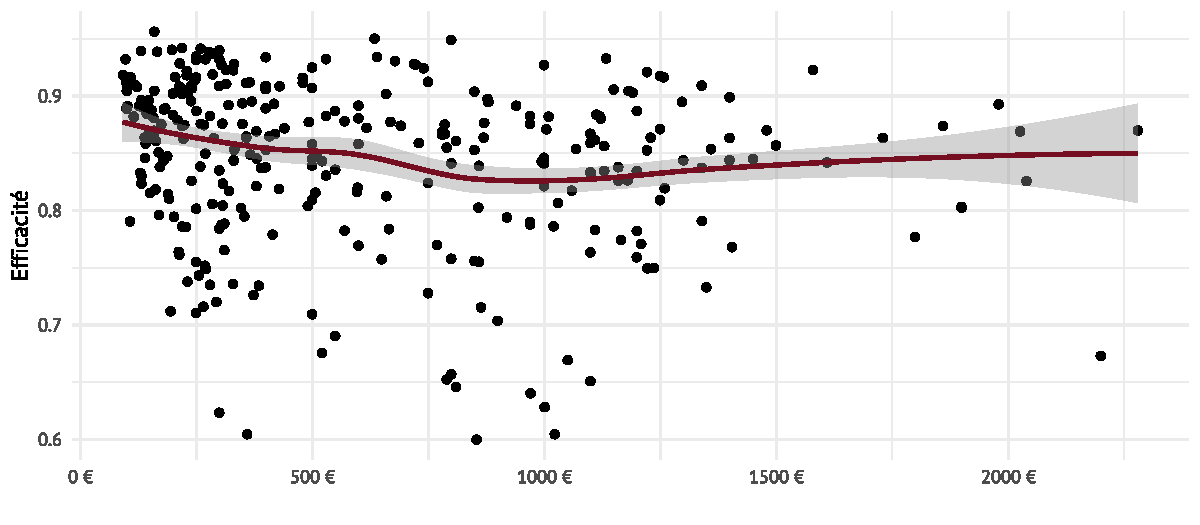
\includegraphics{report_files/figure-pdf/unnamed-chunk-8-1.pdf}

}

\caption{Efficacités en fonction des prix.}

\end{figure}%

On remarque une fois de plus que moins les téléphones sont chers, et
plus ils sont efficaces. Une des explications que nous proposons est
qu'il existe une intensité concurrentielle élevée entre les fabricants
dans cette gamme de prix et peu de marge disponible lorsque le prix est
bas.

\begin{figure}[H]

{\centering 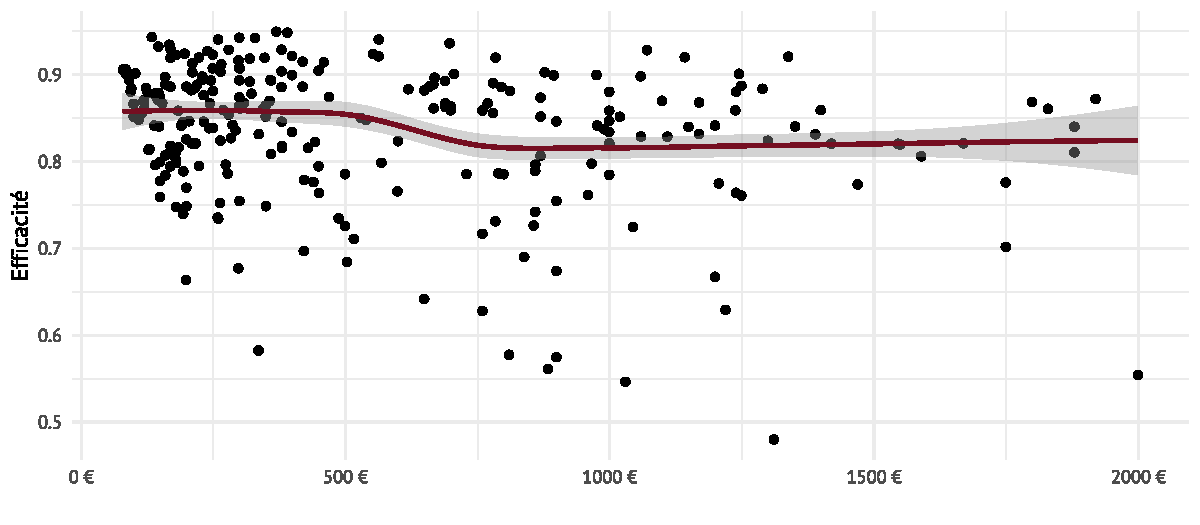
\includegraphics{report_files/figure-pdf/unnamed-chunk-9-1.pdf}

}

\caption{Distribution des efficacités.}

\end{figure}%

La distribution est dite \emph{left skewed}, et l'asymétrie de la
distribution est négative. Il y a beaucoup plus de valeurs concentrées à
droite de la distribution qu'à gauche.

\newpage

\subsection{Analyse Factorielle de Données
Mixtes}\label{analyse-factorielle-de-donnuxe9es-mixtes}

A posteriori, on cherche à synthétiser l'ensemble des variables de notre
modèle de \textbf{Stochastic Cost Frontier}. Pour cela, nous allons
effectuer une analyse factorielle qui nous permet de prendre en compte
simultanément des variables quantitatives et qualitatives en tant que
variables actives : une \textbf{AFDM} (Analyse Factorielle de Données
Mixtes).

\begin{figure}[H]

{\centering 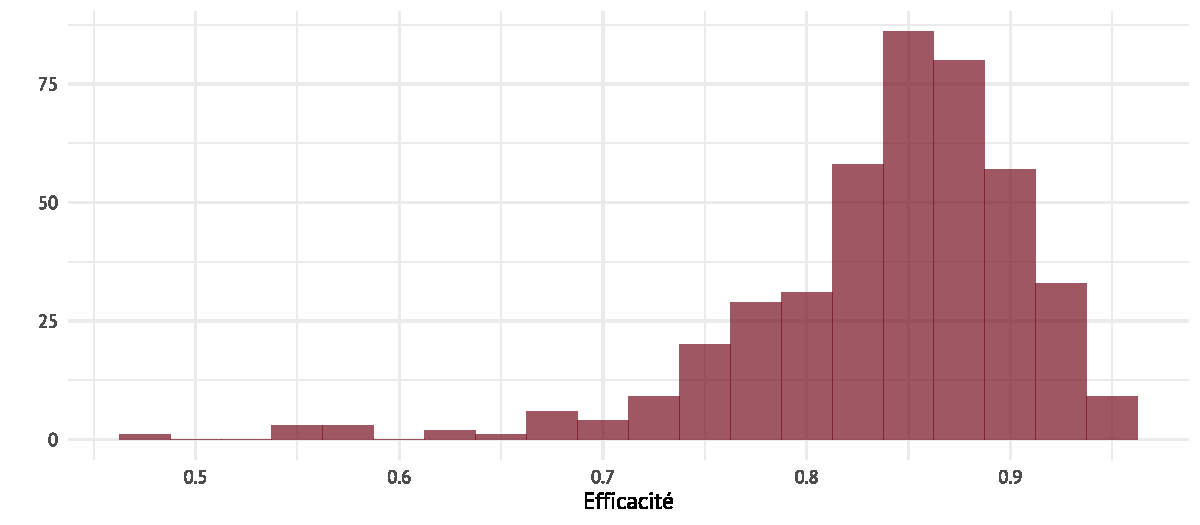
\includegraphics{report_files/figure-pdf/unnamed-chunk-11-1.pdf}

}

\caption{Inerties.}

\end{figure}%

\begin{itemize}
\tightlist
\item
  Sur les quatre premières dimensions, l'inertie cumulée est de
  \textbf{39.65\%}, on peut donc se concentrer sur ces dimensions pour
  notre analyse.
\end{itemize}

\begin{figure}[H]

{\centering 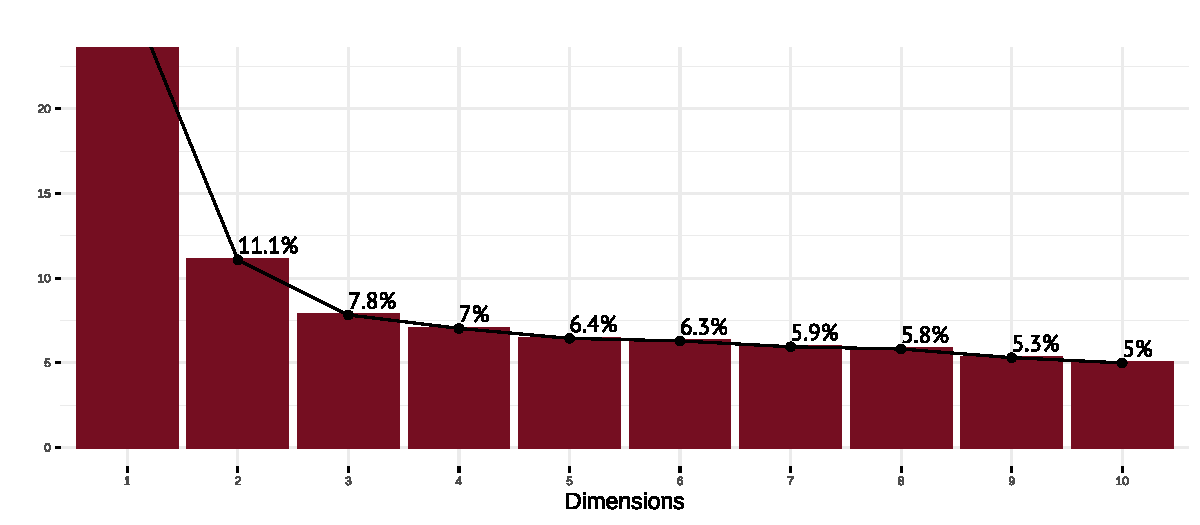
\includegraphics{report_files/figure-pdf/unnamed-chunk-12-1.pdf}

}

\caption{Nuage des individus (Dimension 1 et 2).}

\end{figure}%

\begin{itemize}
\tightlist
\item
  Le nuage des individus dans la dimension 1 et 2 permet de déterminer
  que les téléphones sont assez bien regroupés en fonction de leur
  marque et que les téléphones les moins chers se situent dans la partie
  négative de l'axe 1 tandis que les téléphones les plus chers se
  situent dans la partie positive de l'axe 1.
\end{itemize}

\newpage

\begin{figure}[H]

{\centering 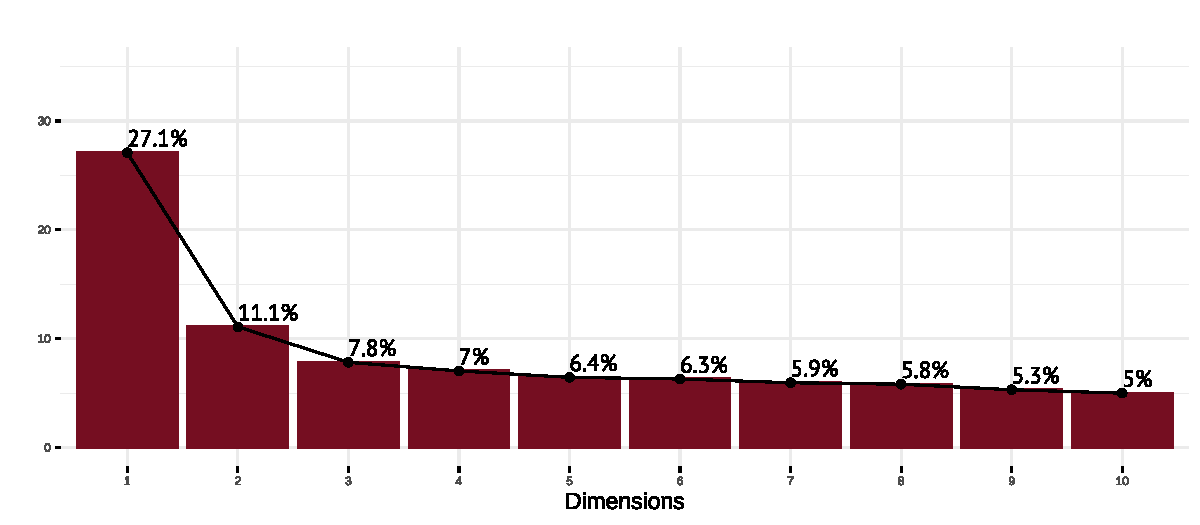
\includegraphics{report_files/figure-pdf/unnamed-chunk-13-1.pdf}

}

\caption{Contribution des variables (Dimensions 1 -- 4).}

\end{figure}%

\begin{itemize}
\item
  Les variables contribuant le plus à la dimension 1 sont
  \emph{logprice}, \emph{upgrade\_storage}, \emph{network},
  \emph{brand}, \emph{induction}, \emph{ram} et \emph{storage}.
\item
  Dans la dimension 2, les proportions de contribution sont elles
  partagées entre 3 variables : \emph{brand}, \emph{screen\_size} et
  \emph{ram}
\item
  Pour la dimension 3 et 4, \emph{brand} est une variable qui contribue
  encore plus à la construction des axes avec plus de 50\% de
  contribution.
\end{itemize}

\begin{figure}[H]

{\centering 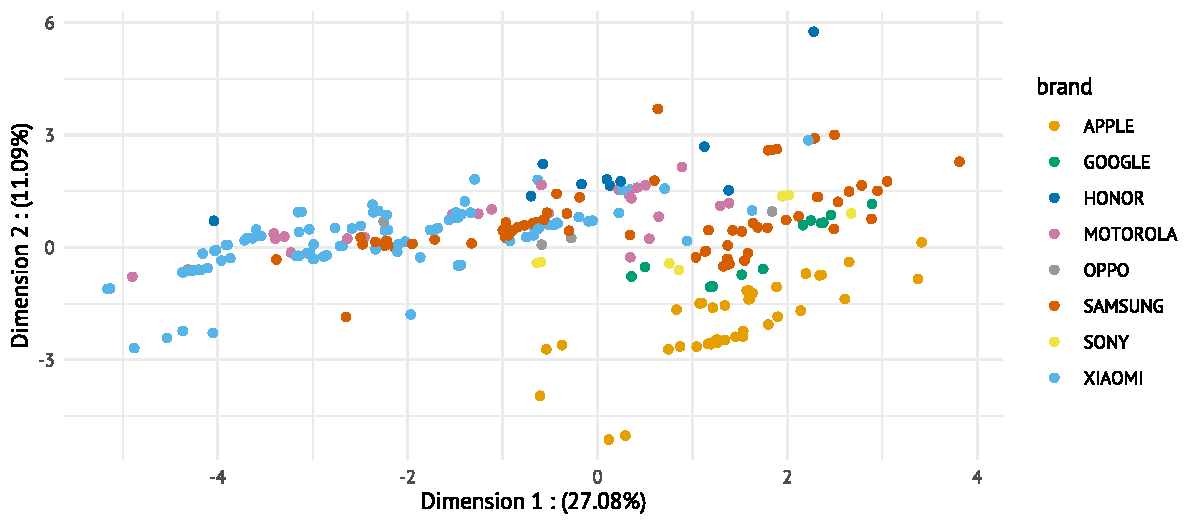
\includegraphics{report_files/figure-pdf/unnamed-chunk-14-1.pdf}

}

\caption{\(\eta^2\) des variables (Dimensions 1 -- 4).}

\end{figure}%

\newpage

Les \(\eta^2\) permettent de distinguer les variables les plus
structurantes d'un axe

\begin{itemize}
\item
  Dans la dimension 1, la variable \emph{logprice} et
  \emph{upgrade\_storage} sont les plus structurantes.
\item
  Dans les dimensions 2,3 et 4, on s'aperçoit que c'est la variable
  \emph{brand} qui est la plus structurante.
\item
  Les variables \emph{ram} et \emph{screen\_size} sont aussi très
  structurantes dans la dimension 2.
\end{itemize}

Opposition entre la marque et le prix (dim 1/2)

\begin{figure}[H]

{\centering 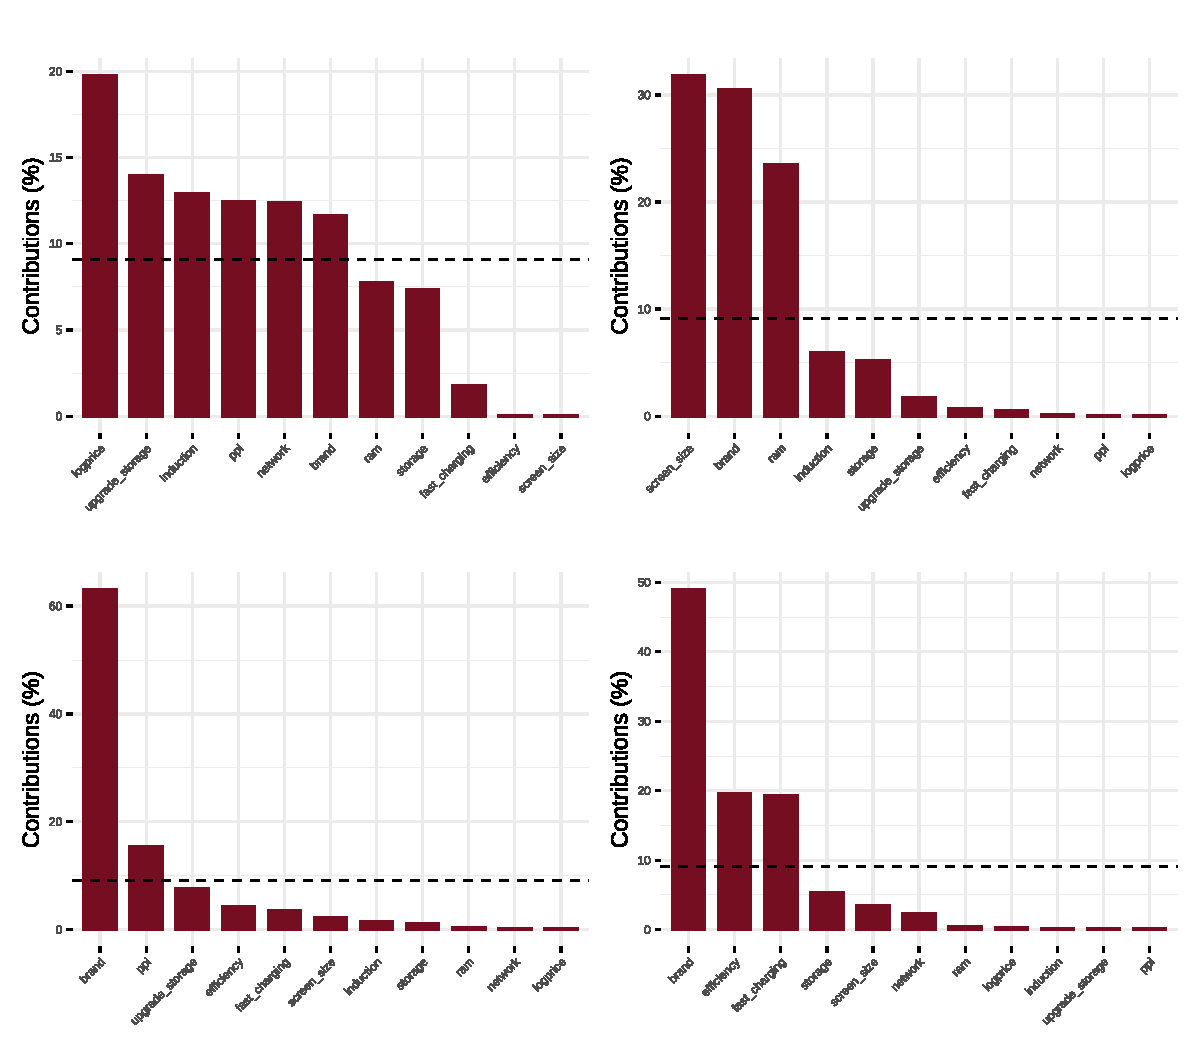
\includegraphics{report_files/figure-pdf/unnamed-chunk-15-1.pdf}

}

\caption{Cercle des corrélations (Dimensions 1 et 2).}

\end{figure}%

D'après le nuage des variables, on peut voir que les variables qui
contribuent à l'axe F1 sont le \emph{logprice}, \emph{ppi},
\emph{storage} ainsi que \emph{ram}. On peut donc supposer que les 3
caractéristiques constituent la majeure partie de la variation observée
dans la variable \emph{logprice}.

Pour l'axe F2, ce sont principalement les variables \emph{screen\_size}
et \emph{efficiency} qui contribuent le plus à cet axe. On peut observer
que l'efficacité (\emph{efficiency}) est moins bien représentée que
\emph{screen\_size}, comme le suggère la différence dans la longueur des
flèches associées à ces variables.

\begin{figure}[H]

{\centering 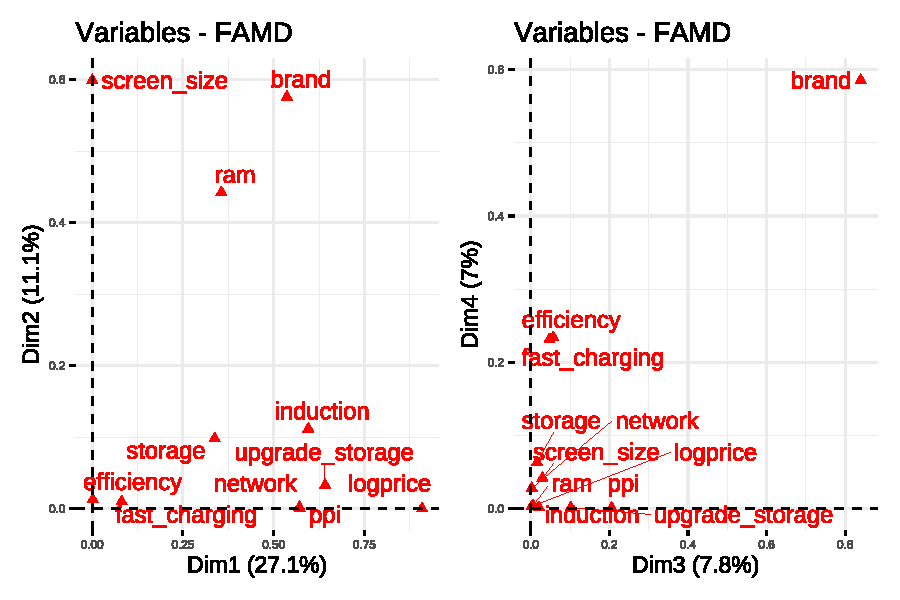
\includegraphics{report_files/figure-pdf/unnamed-chunk-16-1.pdf}

}

\caption{Cercle des corrélations (Dimensions 3 et 4).}

\end{figure}%

Les variables ne contribuent pas beaucoup aux dimensions 3 et 4. Pour
l'axe F3, la \emph{ppi} contribuent pas mal suivi de \emph{storage},
\emph{ram}.

Les variables présentent une contribution relativement faible aux
dimensions 3 et 4 de l'analyse. En ce qui concerne l'axe F3, on constate
que le \textbf{ppi} contribue un peu plus que les autres, suivi par
\emph{storage} et \emph{ram}.

Pour l'axe F4, c'est la variable \emph{screen\_size} qui contribue le
plus, suivie par \emph{efficiency}, tandis que \emph{logprice} contribue
pratiquement pas. Il est également à noter que toutes ces variables sont
positionnées du côté négatif de l'axe.

\chapter{Comparateur}\label{comparateur}

En se basant sur notre problématique, nous voulions, en plus d'une
estimation économétrique qui présente son lot de complexité, créer une
application, et plus précisément un \textbf{comparateur d'efficacité}.

En premier lieu, il convient de se poser une question qui semble
évidente à première vue, mais qui, quand on s'y penche de plus près, est
assez sophistiquée.

\begin{itemize}
\tightlist
\item
  Cette question c'est : \emph{``Qu'est ce qu'un comparateur exactement
  ?''}
\end{itemize}

\begin{tcolorbox}[enhanced jigsaw, colframe=quarto-callout-tip-color-frame, colbacktitle=quarto-callout-tip-color!10!white, left=2mm, rightrule=.15mm, toprule=.15mm, bottomtitle=1mm, breakable, colback=white, titlerule=0mm, coltitle=black, arc=.35mm, opacitybacktitle=0.6, opacityback=0, bottomrule=.15mm, leftrule=.75mm, toptitle=1mm, title=\textcolor{quarto-callout-tip-color}{\faLightbulb}\hspace{0.5em}{Définition}]

\begin{itemize}
\item
  Un comparateur est un site web qui permet de comparer différents
  produits ou services.
\item
  Principalement axé sur les prix, il peut également prendre en compte
  les aspects techniques et la qualité des produits.
\end{itemize}

\end{tcolorbox}

On retrouve l'utilisation des comparateurs dans de nombreux domaines
tels que les comparateurs de vols, d'assurances, de voitures, ou encore
de banques.

En bref il existe une variété de cas d'usage et un nombre croissant
d'utilisateurs faisant appel à ces comparateurs avant d'acheter un bien
ou un service.

D'autre part, il y a des questions juridiques, économiques, statistiques
et algorithmiques qui se posent.

En effet, les opérateurs de plateforme en ligne doivent délivrer au
consommateur une information \textbf{loyale}, \textbf{claire} et
\textbf{transparente}, selon l'article
\href{https://www.legifrance.gouv.fr/codes/article_lc/LEGIARTI000033219601}{L.
111-7 du code de la consommation}.

\textbf{Les comparateurs en ligne sont donc eux aussi soumis à ces
obligations de loyauté et de transparence.}

\begin{enumerate}
\def\labelenumi{\arabic{enumi}.}
\item
  Page dédiée accessible depuis toutes les autres pages du comparateur
  informant le fonctionnement de celui-ci.
\item
  Faire figurer sur chaque page de résultats les informations concernant
  les critères de classement.
\item
  Indiquer via la mention explicite \textbf{« annonce »} les résultats
  liés à des partenariats rémunérés.
\end{enumerate}

Il va sans dire que très peu de comparateurs respectent le premier
point, souvent pour une raison simple : ce sont juste des listings de
prix de téléphones du moins cher au plus cher, donc il n'y a pas
vraiment de fonctionnement à proprement parler. De même, concernant les
critères de classement.

En revanche le troisième point est presque toujours indiqué quelque part
avec la mention \emph{publicité} ou \emph{annonce} quand il y a un
partenariat rémunéré, et c'est normal car une grande partie des revenus
de ces comparateurs provient de ces partenariats donc ils font assez
attention à ce point.

\textbf{\emph{L'avantage de notre comparateur c'est qu'il respecte les
deux premiers points, sans se soucier du troisième puisque nous n'avons
pas de partenariats rémunérés. Tout ça permet d'offrir une grande
transparence pour le consommateur.}}

\section{Smart Specs}\label{smart-specs}

\chapter{Conclusion}\label{conclusion-2}

La réalisation d'une étude utilisant les modèles SFA pour évaluer les
prix des smartphones a permis de mieux comprendre les dynamiques
complexes de ce marché en constante évolution. En explorant la
littérature existante sur la SFA et la régression hédonique des prix,
nous avons découvert les fondements théoriques de ces modèles, leurs
apports ainsi que leurs limites.

Les statistiques descriptives réalisées sur 487 smartphones vendus par
un revendeur français \emph{(octobre 2023)} ont révélé une distribution
étalée des prix, confirmant la nature hautement différenciée des
smartphones. En utilisant des modèles de régression hédonique, nous
avons réussi à prédire avec précision les prix en utilisant différents
types de spécifications, notamment \emph{niveau-niveau} en
\emph{log-niveau}. Ces résultats ont été extrêmement satisfaisants,
démontrant la capacité des modèles à correctement inférer les prix des
smartphones en fonction de leurs caractéristiques.

Cependant, pour aller au-delà de la simple prédiction des prix, nous
avons également appliqué un modèle SFA, spécifiquement la \emph{Cost
Frontier Analysis}, afin d'évaluer l'efficacité des prix des téléphones
en tenant compte de leurs caractéristiques. Cela nous a permis de
déterminer les téléphones offrant le meilleur rapport qualité-prix,
offrant ainsi une perspective supplémentaire dans la compréhension du
pricing de ces téléphones.

La prochaine étape de ce projet consistera à créer une application
comparative. Celle-ci permettra aux utilisateurs \emph{(tout du moins
nous l'espérons)}, de spécifier les caractéristiques recherchées dans un
téléphone. En utilisant le modèle SFA que nous avons développé, un score
sera généré pour chaque téléphone, classant ainsi les appareils du plus
efficace au moins efficace en fonction des critères spécifiés. Cette
application offrira une solution pratique et personnalisée aux
utilisateurs pour prendre des décisions informées lors de l'achat ou de
la production de smartphones.

En résumé, cette étude approfondie combinant la régression hédonique, la
SFA et l'analyse des prix des smartphones a non seulement permis de
prédire précisément les prix en fonction des caractéristiques, mais a
également jeté les bases d'une application offrant des recommandations
personnalisées basées sur l'efficacité des prix des téléphones. Ce
projet ouvre des perspectives intéressantes pour aider les consommateurs
et les producteurs à prendre des décisions éclairées dans un marché
aussi dynamique et complexe que celui des smartphones.

\macrostars

\chapter{Annexe}\label{annexe}

\section{Dérivation de la fonction de
vraisemblance}\label{duxe9rivation-de-la-fonction-de-vraisemblance}

\begin{equation}\phantomsection\label{eq-fv}{
f(v) = \frac{1}{\sqrt{2\pi}\sigma_v}\exp{\left(-\frac{v^2}{2\sigma^2_v} \right)}
}\end{equation}

\begin{equation}\phantomsection\label{eq-fu}{
\begin{gathered}
f(u) = \frac{1}{\sqrt{2\pi}\sigma_u\left[1-\Phi(-\frac{\mu}{\sigma_u})\right]}\exp\left[-\frac{1}{2}\left(\frac{u-\mu}{\sigma_u}\right)^2 \right]\\
= \frac{1}{\sqrt{2\pi}\sigma_u\Phi(\frac{\mu}{\sigma_u})}\exp\left[-\frac{1}{2}\left(\frac{u-\mu}{\sigma_u}\right)^2 \right]
\end{gathered}
}\end{equation}

Etant donné l'hypothèse d'indépendance entre \(u\) et \(v\) :

\begin{equation}\phantomsection\label{eq-fv-fu}{
f(v,u) = f(v) \cdot f(u) = \frac{1}{2\pi\sigma_v\sigma_u\Phi\left(\frac{\mu}{\sigma_u}\right)}\exp\left\{-\frac{1}{2}\left[\frac{v^2}{\sigma^2_v} + \left(\frac{u-\mu}{\sigma_u}\right)^2\right] \right\}
}\end{equation}

Donc,

\begin{equation}\phantomsection\label{eq-fepsilon}{
f(u-\epsilon, u) = \frac{1}{2\pi\sigma_v\sigma_u\Phi\left(\frac{\mu}{\sigma_u}\right)}\exp\left\{-\frac{1}{2}\left[\left(\frac{u-\epsilon}{\sigma_v}\right)^2 + \left(\frac{u-\mu}{\sigma_u}\right)^2\right] \right\}
}\end{equation}

Cette expression peut être simplifiée. Notez que :

\begin{equation}\phantomsection\label{eq-fepsilon-2}{
\left(\frac{u-\epsilon}{\sigma_v}\right)^2 + \left(\frac{u-\mu}{\sigma_u}\right)^2 = \frac{\sigma^2_v + \sigma^2_u}{\sigma^2_v\sigma^2_u}\left[u^2 - 2u \left( \frac{\mu\sigma^2_v+\epsilon\sigma^2_u}{\sigma^2_v+\sigma^2_u}\right)\right] + \left(\frac{\mu^2}{\sigma^2_u}-\frac{\epsilon^2}{\sigma^2_v}\right)
}\end{equation}

Définissons :

\[
\mu_* = \frac{\mu\sigma^2_v+\epsilon\sigma^2_u}{\sigma^2_v+\sigma^2_u}
\]

\[
\sigma^2_* = \frac{\sigma^2_v\sigma^2_u}{\sigma^2_v + \sigma^2_u}
\]

Dès lors, l'équation~\ref{eq-fepsilon} est simplifiée pour obtenir :

\begin{equation}\phantomsection\label{eq-fepsilon-3}{
f(u-\epsilon, u) = \frac{1}{2\pi\sigma_v\sigma_u\Phi\left(\frac{\mu}{\sigma_u}\right)}\exp\left\{-\frac{1}{2}\left[\left(\frac{u-\mu_*}{\sigma_*}\right)^2+\frac{\left(\mu - \epsilon\right)^2}{\sigma^2_u+\sigma^2_v}\right]\right\}
}\end{equation}

Alors, la densité de \(f(\epsilon)\) est :

\[
f(\epsilon) = \int_0^{\infty}f(u-\epsilon, u)du
\]

\[
\dots
\]

\begin{equation}\phantomsection\label{eq-fepsilon-4}{
f(\epsilon) = \frac{\phi\left(\frac{\mu - \epsilon}{\sqrt{\sigma^2_v+\sigma^2_u}}\right)}{\sqrt{\sigma^2_v+\sigma^2_u}\left[\frac{\Phi\left(\frac{\mu}{\sigma_u}\right)}{\Phi\left(\frac{\mu_*}{\sigma_*}\right)}\right]}
}\end{equation}

En prenant le logarithme de l'équation précédente, on obtient la
fonction de log-vraisemblance pour une observation \(i\) dans le cadre
d'un modèle avec loi normale tronquée.

\begin{equation}\phantomsection\label{eq-log-likelihood}{
L_i = - \frac{1}{2}\ln\left(\sigma^2_v+\sigma^2_u\right) + \ln \phi \left(\frac{\mu - \epsilon}{\sqrt{\sigma^2_v+\sigma^2_u}}\right) + \ln \Phi \left(\frac{\mu_*}{\sigma_*}\right) - \ln \Phi\left(\frac{\mu}{\sigma_u}\right)
}\end{equation}

\section{Dérivation des indices
d'efficacité}\label{duxe9rivation-des-indices-defficacituxe9}

\begin{equation}\phantomsection\label{eq-f-u-epsilon}{
f(u|\epsilon) = \frac{1}{\sqrt{2 \pi}\sigma_* \Phi(\frac{\mu_*}{\sigma_*})} \exp\left[- \frac{1}{2}\left(\frac{u - \mu_*}{\sigma_*}\right)^2\right]
}\end{equation}

Avec \(\mu_*\) et \(\sigma_*\) définis plus haut :

\begin{equation}\phantomsection\label{eq-expected-u-epsilon}{
E(u | \epsilon) =  \int_{0}^{\infty} \frac{u}{\sqrt{2 \pi}\sigma_* \Phi(\frac{\mu_*}{\sigma_*})} \exp\left[- \frac{1}{2}\left(\frac{u - \mu_*}{\sigma_*}\right)^2\right] du
}\end{equation}

Définissions :

\[
w = \frac{u - \mu_*}{\sigma_*},   w \in \left[ -\frac{\mu_*}{\sigma_*}, \infty \right), dw = \frac{du}{\sigma_*}
\]

Donc :

\[
E(u | \epsilon) =  \int_{- \frac{\mu_*}{\sigma_*}}^{\infty} \frac{\mu_* + w\sigma_*}{\sqrt{2 \pi} \Phi \left(\frac{\mu_*}{\sigma_*}\right)} \exp \left(- \frac{1}{2} w^2 \right) dw
\] \[
= \frac{\mu_*}{\Phi \left(\frac{\mu_*}{\sigma_*}\right)} \int_{- \frac{\mu_*}{\sigma_*}}^{\infty} \frac{1}{\sqrt{2 \pi}} \exp \left(- \frac{1}{2} w^2 \right)dw + \frac{\sigma_*}{\Phi \left(\frac{\mu_*}{\sigma_*} \right)} \int_{- \frac{\mu_*}{\sigma_*}}^{\infty} \frac{w}{\sqrt{2 \pi}} \exp \left(- \frac{1}{2} w^2 \right)dw\\
\]

\[
= \mu_* + \frac{\sigma_*}{\Phi \left(\frac{\mu_*}{\sigma_*} \right)} \cdot \frac{1}{\sqrt{2 \pi}} \exp \left[- \frac{1}{2} \left(\frac{\mu_*}{\sigma_*} \right)^2 \right]\\
\]

\[
= \mu_* + \frac{\phi \frac{\mu_*}{\sigma_*}}{\Phi \frac{\mu_*}{\sigma_*}} \sigma_*
\]

Maintenant, pour \(E(\exp(- u) | \epsilon)\),

\[
E(\exp(- u)| \epsilon) = \int_{0}^{\infty} \exp(-u) f(u | \epsilon) du 
\]

\[
= \int_{0}^{\infty} \frac{1}{\sqrt{2 \pi}\sigma_* \Phi(\frac{\mu_*}{\sigma_*})} \exp\left[- \frac{1}{2}\left(\frac{u - \mu_*}{\sigma_*}\right)^2 - u\right] du
\]

\[
= \frac{1}{\sigma_* \Phi(\frac{\mu_*}{\sigma_*})} \int_{0}^{\infty} \frac{1}{\sqrt{2 \pi}} \exp \left[- \frac{1}{2}\left(\frac{u - \mu_*}{\sigma_*}\right)^2 - u\right]du
\]

Notons que

\[
- \frac{1}{2}\left(\frac{u - \mu_*}{\sigma_*}\right)^2 - u = - \frac{[u - ( \mu_* - \sigma_*^2)]^2}{2 \sigma_*^2} - \frac{1}{2} (2\mu_* - \sigma_*)
\]

Dès lors, on peut simplifier la formule :

\[
E(\exp(-u) | \epsilon) = \frac{1}{\sigma_* \Phi(\frac{\mu_*}{\sigma_*})}  \int_{0}^{\infty} \frac{1}{\sqrt{2 \pi}} \exp \left\{ - \frac{[ u - ( \mu_* - \sigma_*^2)]^2}{2 \sigma_*^2} - \frac{1}{2} (2\mu_* - \sigma_*^2)\right\} du
\]

\[
= \frac{\exp \left[- \frac{1}{2} (2\mu_* - \sigma_*^2) \right]}{\sigma_* \Phi (\frac{\mu_*}{\sigma_*})}  \int_{0}^{\infty} \frac{1}{\sqrt{2 \pi}} \exp \left\{-\frac{1}{2} \left[\frac{u - (\mu_* - \sigma_*^2)}{\sigma_*} \right]^2 \right\}du
\]

Définissons :

\[
z = \frac{u - (\mu_* - \sigma_*^2)}{\sigma_*}, z \in \left[ -\frac{\mu_*}{\sigma_*} + \sigma_*, \infty \right), dz = \frac{du}{\sigma_*}
\]

Enfin,

\[
E(\exp(-u)| \epsilon) = \frac{\exp \left[- \frac{1}{2} (2\mu_* - \sigma_*^2) \right]}{\sigma_* \Phi (\frac{\mu_*}{\sigma_*})} \int_{-\frac{\mu_*}{\sigma_*} + \sigma_*}^{\infty} \frac{1}{\sqrt{2 \pi}} \exp \left\{ - \frac{1}{2} z^2\right\} dz
\]

\[
= \exp \left(-\mu_* + \frac{1}{2} \sigma_*^2 \right) \frac{\Phi \left(\frac{\mu_*}{\sigma_*} - \sigma_* \right)}{\Phi\frac{\mu_*}{\sigma_*}}
\]

\chapter{Acronymes}\label{acronymes}

\begin{description}
\item[WTP]
Willingness To Pay
\item[SFA]
Stochastic Frontier Analysis
\item[DAS]
Débit d'Absoprtion Spécifique
\item[DEA]
Data Envelopment Analysis
\item[TE]
Technical Efficiency
\item[BLUE]
Best Linear Unbiased Estimator
\item[MCO]
Moindres Carrés Ordinaires
\item[MV]
Maximum de Vraisemblance
\end{description}

\chapter{Glossaire des variables}\label{glossaire-des-variables}

\begin{description}
\item[\emph{screen\_type}]
Type d'écran : Plat, Pliable, etc. \(\Rightarrow\) \texttt{str}
\item[\emph{screen\_size}]
Taille de l'écran, en pouces \(\Rightarrow\) \texttt{float}
\item[\emph{screen\_tech}]
Technologie de l'écran : LCD, OLED, AMOLED. \(\Rightarrow\) \texttt{str}
\item[\emph{resolution\_1/2}]
Résolution verticale/horizontale de l'écran, en nombre de pixels
\(\Rightarrow\) \texttt{int}
\item[\emph{diagonal\_pixels}]
Diagonale en nombre de pixels calculée à partir de la résolution
\(\Rightarrow\) \texttt{float}
\item[\emph{ppi}]
Pixels Per Inch, calculé à partir de la diagonale et de la taille de
l'écran \(\Rightarrow\) \texttt{float}
\item[\emph{cam\_1, cam\_2, cam\_3}]
Résolution de la caméra 1/2/3 en mégapixels \(\Rightarrow\) \texttt{int}
\item[\emph{mpx\_backward\_cam}]
Somme des résolutions des caméras 1, 2 et 3 en mégapixels
\(\Rightarrow\) \texttt{ìnt}
\item[\emph{sensor}]
Nombre de caméras arrières équipées sur le téléphone \(\Rightarrow\)
\texttt{int}
\item[\emph{color}]
Couleur du téléphone \(\Rightarrow\) \texttt{str}
\item[\emph{thickness}]
Epaisseur du téléphone en millimètres \(\Rightarrow\) \texttt{float}
\item[\emph{width}]
Largeur du téléphone en millimètres \(\Rightarrow\) \texttt{float}
\item[\emph{height}]
Hauteur du téléphone en millimètres \(\Rightarrow\) \texttt{float}
\item[\emph{net\_weight}]
Poids net du téléphone en grammes \(\Rightarrow\) \texttt{float}
\item[\emph{network}]
Prise en charge réseau jusqu'à la 4G ou la 5G \(\Rightarrow\)
\texttt{str}
\item[\emph{cpu}]
Type de CPU. \emph{Variable Inexploitable} \(\Rightarrow\) \texttt{str}
\item[\emph{ram}]
Capacité de RAM en Gigaoctets \(\Rightarrow\) \texttt{int}
\item[\emph{storage}]
Capacité de stockage en Gigaoctets \(\Rightarrow\) \texttt{int}
\item[\emph{upgrade\_storage}]
L'appareil dispose t-il d'un moyen d'augmenter son stockage
\(\Rightarrow\) \texttt{bool}
\item[\emph{battery}]
Capacité de la batterie en milliampères \(\Rightarrow\) \texttt{int}
\item[\emph{fast\_charging}]
L'appareil dispose t-il d'une charge rapide \(\Rightarrow\)
\texttt{bool}
\item[\emph{induction}]
L'appareil dispose t-il d'une charge par induction \(\Rightarrow\)
\texttt{bool}
\item[\emph{usb\_type\_c}]
L'appareil dispose t-il d'un port USB type C \(\Rightarrow\)
\texttt{bool}
\item[\emph{repairability\_index}]
Indice de réparabilité du téléphone (Note /10) \(\Rightarrow\)
\texttt{int}
\item[\emph{model}]
Modèle du téléphone \(\Rightarrow\) \texttt{str}
\item[\emph{brand}]
Marque du téléphone \(\Rightarrow\) \texttt{str}
\item[\emph{made\_in}]
Lieu de fabrication du téléphone \(\Rightarrow\) \texttt{str}
\item[\emph{stars}]
Note sur 5 du téléphone (quand disponible) \(\Rightarrow\)
\texttt{float}
\item[\emph{reviews}]
Nombre de critiques \(\Rightarrow\) \texttt{int}
\item[\emph{das\_head/chest/limbs}]
Débit d'absorption spécifique tête/corps/membres \(\Rightarrow\)
\texttt{float}
\item[\emph{price}]
Prix du téléphone \(\Rightarrow\) \texttt{float}
\end{description}

\chapter{Licence}\label{licence}

\begin{tcolorbox}[enhanced jigsaw, colframe=quarto-callout-warning-color-frame, colbacktitle=quarto-callout-warning-color!10!white, left=2mm, rightrule=.15mm, toprule=.15mm, bottomtitle=1mm, breakable, colback=white, titlerule=0mm, coltitle=black, arc=.35mm, opacitybacktitle=0.6, opacityback=0, bottomrule=.15mm, leftrule=.75mm, toptitle=1mm, title=\textcolor{quarto-callout-warning-color}{\faExclamationTriangle}\hspace{0.5em}{\textbf{Licence CC BY-NC-SA 4.0} \textbar{}
\faIcon{creative-commons}\faIcon{creative-commons-by}\faIcon{creative-commons-nc}\faIcon{creative-commons-sa}}]

\textbf{Vous êtes autorisé à :}

\vspace{1em}

\begin{quote}
\textbf{Partager} --- copier, distribuer et communiquer le matériel par
tous moyens et sous tous formats.
\end{quote}

\vspace{1em}

\begin{quote}
\textbf{Adapter} --- remixer, transformer et créer à partir du matériel.
\end{quote}

\vspace{1em}

\begin{quote}
L'Offrant ne peut retirer les autorisations concédées par la licence
tant que vous appliquez les termes de cette licence.
\end{quote}

\vspace{1em}

\textbf{Selon les conditions suivantes :}

\vspace{1em}

\begin{quote}
\faIcon{creative-commons-by} \textbf{Attribution} --- Vous devez
créditer l'Œuvre, intégrer un lien vers la licence et indiquer si des
modifications ont été effectuées à l'Oeuvre. Vous devez indiquer ces
informations par tous les moyens raisonnables, sans toutefois suggérer
que l'Offrant vous soutient ou soutient la façon dont vous avez utilisé
son Oeuvre.
\end{quote}

\vspace{1em}

\begin{quote}
\faIcon{creative-commons-nc} \textbf{Pas d'Utilisation Commerciale} ---
Vous n'êtes pas autorisé à faire un usage commercial de cette Oeuvre,
tout ou partie du matériel la composant.
\end{quote}

\vspace{1em}

\begin{quote}
\faIcon{creative-commons-sa} \textbf{Partage dans les Mêmes Conditions}
--- Dans le cas où vous effectuez un remix, que vous transformez, ou
créez à partir du matériel composant l'Oeuvre originale, vous devez
diffuser l'Oeuvre modifiée dans les même conditions, c'est à dire avec
la même licence avec laquelle l'Oeuvre originale a été diffusée.
\end{quote}

\vspace{1em}

\begin{quote}
\textbf{Pas de restrictions complémentaires} --- Vous n'êtes pas
autorisé à appliquer des conditions légales ou des mesures techniques
qui restreindraient légalement autrui à utiliser l'Oeuvre dans les
conditions décrites par la licence.
\end{quote}

\vspace{1em}

\url{https://creativecommons.org/licenses/by-nc-sa/4.0/deed.fr}

\end{tcolorbox}

\chapter*{Références}\label{ruxe9fuxe9rences}
\addcontentsline{toc}{chapter}{Références}

\phantomsection\label{refs}
\begin{CSLReferences}{1}{0}
\bibitem[\citeproctext]{ref-ahmad2019}
Ahmad, Waseem, Tanvir Ahmed, et Bashir Ahmad. 2019. {«~Pricing of mobile
phone attributes at the retail level in a developing country: Hedonic
analysis~»}. \emph{Telecommunications Policy} 43 (4): 299‑309.
\url{https://doi.org/10.1016/j.telpol.2018.10.002}.

\bibitem[\citeproctext]{ref-aigner1977}
Aigner, Dennis, C. A.Knox Lovell, et Peter Schmidt. 1977. {«~Formulation
and estimation of stochastic frontier production function models~»}.
\emph{Journal of Econometrics} 6 (1): 21‑37.
\url{https://doi.org/10.1016/0304-4076(77)90052-5}.

\bibitem[\citeproctext]{ref-arrondo2018}
Arrondo, Ruben, Nuria Garcia, et Eduardo Gonzalez. 2018. {«~Estimating
product efficiency through a hedonic pricing best practice frontier~»}.
\emph{BRQ Business Research Quarterly} 21 (4): 215‑24.
\url{https://doi.org/10.1016/j.brq.2018.08.005}.

\bibitem[\citeproctext]{ref-bello2010}
Bello, Ajide K, et Alabi Moruf. 2010. {«~Does the functional form matter
in the estimation of hedonic price model for housing market~»}.
\emph{The Social Sciences} 5 (6): 559‑64.

\bibitem[\citeproctext]{ref-berndt2001}
Berndt, Ernst R, et Neal J Rappaport. 2001. {«~Price and quality of
desktop and mobile personal computers: A quarter-century historical
overview~»}. \emph{American Economic Review} 91 (2): 268‑73.
\url{https://www.aeaweb.org/articles?id=10.1257/aer.91.2.268}.

\bibitem[\citeproctext]{ref-boistel2008}
Boistel, Philippe. 2008. {«~La r{é}putation d'entreprise: un impact
majeur sur les ressources de l'entreprise~»}. \emph{Revue management et
avenir}, nᵒ 3: 9‑25.

\bibitem[\citeproctext]{ref-chen2010}
Chen, Ching-Fu, et Rochelle Rothschild. 2010. {«~An application of
hedonic pricing analysis to the case of hotel rooms in Taipei~»}.
\emph{Tourism Economics} 16 (3): 685‑94.
\url{https://journals.sagepub.com/doi/abs/10.5367/000000010792278310}.

\bibitem[\citeproctext]{ref-efroymson1960}
Efroymson, Michael Alin. 1960. {«~Multiple regression analysis~»}.
\emph{Mathematical methods for digital computers}, 191‑203.

\bibitem[\citeproctext]{ref-farrell1957}
Farrell, Michael James. 1957. {«~The measurement of productive
efficiency~»}. \emph{Journal of the Royal Statistical Society Series A:
Statistics in Society} 120 (3): 253‑81.

\bibitem[\citeproctext]{ref-harrison1978}
Harrison Jr, David, et Daniel L Rubinfeld. 1978. {«~Hedonic housing
prices and the demand for clean air~»}. \emph{Journal of environmental
economics and management} 5 (1): 81‑102.
\url{https://doi.org/10.1016/0095-0696(78)90006-2}.

\bibitem[\citeproctext]{ref-kumbhakar2015}
Kumbhakar, Subal, Alan Horncastle, et al. 2015. \emph{A practitioner's
guide to stochastic frontier analysis using Stata}. Cambridge University
Press.

\bibitem[\citeproctext]{ref-lancaster1966}
Lancaster, Kelvin J. 1966. {«~A New Approach to Consumer Theory~»}.
\emph{Journal of Political Economy} 74 (2): 132‑57.
\url{https://doi.org/10.1086/259131}.

\bibitem[\citeproctext]{ref-mohamad2008}
Mohamad, Shamsher, Taufiq Hassan, et Mohamed Khaled I Bader. 2008.
{«~Efficiency of conventional versus Islamic Banks: international
evidence using the Stochastic Frontier Approach (SFA)~»}. \emph{Journal
of Islamic economics, banking and finance} 4 (2): 107‑30.

\bibitem[\citeproctext]{ref-reinhard2000}
Reinhard, Stijn, CA Knox Lovell, et Geert J Thijssen. 2000.
{«~Environmental efficiency with multiple environmentally detrimental
variables; estimated with SFA and DEA~»}. \emph{European Journal of
Operational Research} 121 (2): 287‑303.

\bibitem[\citeproctext]{ref-rosen1974}
Rosen, Sherwin. 1974. {«~Hedonic Prices and Implicit Markets: Product
Differentiation in Pure Competition~»}. \emph{Journal of Political
Economy} 82 (1): 34‑55. \url{http://www.jstor.org/stable/1830899}.

\bibitem[\citeproctext]{ref-rosko2008}
Rosko, Michael D, et Ryan L Mutter. 2008. {«~Stochastic frontier
analysis of hospital inefficiency: a review of empirical issues and an
assessment of robustness~»}. \emph{Medical care research and review} 65
(2): 131‑66. \url{https://doi.org/10.1177/1077558707307580}.

\bibitem[\citeproctext]{ref-yim2014}
Yim, Eun Soon, Suna Lee, et Woo Gon Kim. 2014. {«~Determinants of a
restaurant average meal price: An application of the hedonic pricing
model~»}. \emph{International Journal of Hospitality Management} 39:
11‑20.
\url{https://www.sciencedirect.com/science/article/abs/pii/S027843191400019X}.

\end{CSLReferences}



\end{document}
